\documentclass[a4paper]{book}
\usepackage{makeidx}
\usepackage{graphicx}
\usepackage{multicol}
\usepackage{float}
\usepackage{listings}
\usepackage{color}
\usepackage{ifthen}
\usepackage[table]{xcolor}
\usepackage{textcomp}
\usepackage{alltt}
\usepackage{ifpdf}
\ifpdf
\usepackage[pdftex,
            pagebackref=true,
            colorlinks=true,
            linkcolor=blue,
            unicode
           ]{hyperref}
\else
\usepackage[ps2pdf,
            pagebackref=true,
            colorlinks=true,
            linkcolor=blue,
            unicode
           ]{hyperref}
\usepackage{pspicture}
\fi
\usepackage[utf8]{inputenc}
\usepackage{mathptmx}
\usepackage[scaled=.90]{helvet}
\usepackage{courier}
\usepackage{doxygen}
\lstset{language=C++,inputencoding=utf8,basicstyle=\footnotesize,breaklines=true,breakatwhitespace=true,tabsize=4,numbers=left }
\makeindex
\setcounter{tocdepth}{3}
\renewcommand{\footrulewidth}{0.4pt}
\begin{document}
\hypersetup{pageanchor=false}
\begin{titlepage}
\vspace*{7cm}
\begin{center}
{\Large Cassandra PHP Client Library }\\
\vspace*{1cm}
{\large Generated by Doxygen 1.7.3}\\
\vspace*{0.5cm}
{\small Mon Jul 4 2011 14:35:59}\\
\end{center}
\end{titlepage}
\clearemptydoublepage
\pagenumbering{roman}
\tableofcontents
\clearemptydoublepage
\pagenumbering{arabic}
\hypersetup{pageanchor=true}
\chapter{Namespace Index}
\section{Namespace List}
Here is a list of all documented namespaces with brief descriptions:\begin{DoxyCompactList}
\item\contentsline{section}{\hyperlink{namespaceCassandra}{Cassandra} }{\pageref{namespaceCassandra}}{}
\end{DoxyCompactList}

\chapter{Data Structure Index}
\section{Class Hierarchy}
This inheritance list is sorted roughly, but not completely, alphabetically:\begin{DoxyCompactList}
\item \contentsline{section}{Cassandra}{\pageref{classCassandra}}{}
\item \contentsline{section}{CassandraCluster}{\pageref{classCassandraCluster}}{}
\item \contentsline{section}{CassandraColumnFamily}{\pageref{classCassandraColumnFamily}}{}
\item \contentsline{section}{CassandraColumnFamilyNotFoundException}{\pageref{classCassandraColumnFamilyNotFoundException}}{}
\item \contentsline{section}{CassandraConnection}{\pageref{classCassandraConnection}}{}
\item \contentsline{section}{CassandraConnectionClosedException}{\pageref{classCassandraConnectionClosedException}}{}
\item \contentsline{section}{CassandraConnectionFailedException}{\pageref{classCassandraConnectionFailedException}}{}
\item \contentsline{section}{CassandraDataIterator}{\pageref{classCassandraDataIterator}}{}
\begin{DoxyCompactList}
\item \contentsline{section}{CassandraIndexedDataIterator}{\pageref{classCassandraIndexedDataIterator}}{}
\item \contentsline{section}{CassandraRangeDataIterator}{\pageref{classCassandraRangeDataIterator}}{}
\end{DoxyCompactList}
\item \contentsline{section}{CassandraInvalidPatternException}{\pageref{classCassandraInvalidPatternException}}{}
\item \contentsline{section}{CassandraInvalidRequestException}{\pageref{classCassandraInvalidRequestException}}{}
\item \contentsline{section}{CassandraMaxRetriesException}{\pageref{classCassandraMaxRetriesException}}{}
\item \contentsline{section}{CassandraSettingKeyspaceFailedException}{\pageref{classCassandraSettingKeyspaceFailedException}}{}
\item \contentsline{section}{CassandraUnsupportedException}{\pageref{classCassandraUnsupportedException}}{}
\item \contentsline{section}{CassandraUtil}{\pageref{classCassandraUtil}}{}
\end{DoxyCompactList}

\chapter{Data Structure Index}
\section{Data Structures}
Here are the data structures with brief descriptions:\begin{DoxyCompactList}
\item\contentsline{section}{\hyperlink{classCassandra}{Cassandra} }{\pageref{classCassandra}}{}
\item\contentsline{section}{\hyperlink{classCassandraCluster}{CassandraCluster} }{\pageref{classCassandraCluster}}{}
\item\contentsline{section}{\hyperlink{classCassandraColumnFamily}{CassandraColumnFamily} }{\pageref{classCassandraColumnFamily}}{}
\item\contentsline{section}{\hyperlink{classCassandraColumnFamilyNotFoundException}{CassandraColumnFamilyNotFoundException} }{\pageref{classCassandraColumnFamilyNotFoundException}}{}
\item\contentsline{section}{\hyperlink{classCassandraConnection}{CassandraConnection} }{\pageref{classCassandraConnection}}{}
\item\contentsline{section}{\hyperlink{classCassandraConnectionClosedException}{CassandraConnectionClosedException} }{\pageref{classCassandraConnectionClosedException}}{}
\item\contentsline{section}{\hyperlink{classCassandraConnectionFailedException}{CassandraConnectionFailedException} }{\pageref{classCassandraConnectionFailedException}}{}
\item\contentsline{section}{\hyperlink{classCassandraDataIterator}{CassandraDataIterator} }{\pageref{classCassandraDataIterator}}{}
\item\contentsline{section}{\hyperlink{classCassandraIndexedDataIterator}{CassandraIndexedDataIterator} }{\pageref{classCassandraIndexedDataIterator}}{}
\item\contentsline{section}{\hyperlink{classCassandraInvalidPatternException}{CassandraInvalidPatternException} }{\pageref{classCassandraInvalidPatternException}}{}
\item\contentsline{section}{\hyperlink{classCassandraInvalidRequestException}{CassandraInvalidRequestException} }{\pageref{classCassandraInvalidRequestException}}{}
\item\contentsline{section}{\hyperlink{classCassandraMaxRetriesException}{CassandraMaxRetriesException} }{\pageref{classCassandraMaxRetriesException}}{}
\item\contentsline{section}{\hyperlink{classCassandraRangeDataIterator}{CassandraRangeDataIterator} }{\pageref{classCassandraRangeDataIterator}}{}
\item\contentsline{section}{\hyperlink{classCassandraSettingKeyspaceFailedException}{CassandraSettingKeyspaceFailedException} }{\pageref{classCassandraSettingKeyspaceFailedException}}{}
\item\contentsline{section}{\hyperlink{classCassandraUnsupportedException}{CassandraUnsupportedException} }{\pageref{classCassandraUnsupportedException}}{}
\item\contentsline{section}{\hyperlink{classCassandraUtil}{CassandraUtil} }{\pageref{classCassandraUtil}}{}
\end{DoxyCompactList}

\chapter{Namespace Documentation}
\hypertarget{namespaceCassandra}{
\section{Cassandra Namespace Reference}
\label{namespaceCassandra}\index{Cassandra@{Cassandra}}
}


\subsection{Detailed Description}
Cassandra-\/PHP-\/Client.

\hyperlink{classCassandra}{Cassandra} PHP-\/based client library for managing and querying your \hyperlink{classCassandra}{Cassandra} cluster. It's a high-\/level library performing all the rather complex low-\/level lifting and providing a simple to learn and use interface.

Includes ideas and code snippets from PHPCassa project.

Copyright (C) 2011 by Priit Kallas $<$\href{mailto:kallaspriit@gmail.com}{\tt kallaspriit@gmail.com}$>$

Permission is hereby granted, free of charge, to any person obtaining a copy of this software and associated documentation files (the \char`\"{}Software\char`\"{}), to deal in the Software without restriction, including without limitation the rights to use, copy, modify, merge, publish, distribute, sublicense, and/or sell copies of the Software, and to permit persons to whom the Software is furnished to do so, subject to the following conditions:

The above copyright notice and this permission notice shall be included in all copies or substantial portions of the Software.

THE SOFTWARE IS PROVIDED \char`\"{}AS IS\char`\"{}, WITHOUT WARRANTY OF ANY KIND, EXPRESS OR IMPLIED, INCLUDING BUT NOT LIMITED TO THE WARRANTIES OF MERCHANTABILITY, FITNESS FOR A PARTICULAR PURPOSE AND NONINFRINGEMENT. IN NO EVENT SHALL THE AUTHORS OR COPYRIGHT HOLDERS BE LIABLE FOR ANY CLAIM, DAMAGES OR OTHER LIABILITY, WHETHER IN AN ACTION OF CONTRACT, TORT OR OTHERWISE, ARISING FROM, OUT OF OR IN CONNECTION WITH THE SOFTWARE OR THE USE OR OTHER DEALINGS IN THE SOFTWARE.

\begin{DoxyAuthor}{Author}
Priit Kallas $<$\href{mailto:kallaspriit@gmail.com}{\tt kallaspriit@gmail.com}$>$
\end{DoxyAuthor}
\begin{DoxyVersion}{Version}
1.0 
\end{DoxyVersion}

\chapter{Data Structure Documentation}
\hypertarget{classCassandra}{
\section{Cassandra Class Reference}
\label{classCassandra}\index{Cassandra@{Cassandra}}
}
\subsection*{Public Member Functions}
\begin{DoxyCompactItemize}
\item 
\hyperlink{classCassandra_abb13b5073e065e8f2a60b1c6f18c573e}{\_\-\_\-clone} ()
\item 
\hyperlink{classCassandra_a4502befdb4278113462bc7fcfbafa09f}{useKeyspace} (\$keyspace, \$username=null, \$password=null)
\item 
\hyperlink{classCassandra_ad8fe43e1ceb9841cca92cf981fb566b3}{getCluster} ()
\item 
\hyperlink{classCassandra_ac300f4b8ed3a2d80388225e0ec990883}{getConnection} ()
\item 
\hyperlink{classCassandra_a382ebe135b67bddef1e0a9fa21448cde}{closeConnections} ()
\item 
\hyperlink{classCassandra_a4eaaed3e996a26cc145057487036584b}{getClient} ()
\item 
\hyperlink{classCassandra_aea614dd2c8170609c0ec9e81607983a0}{setMaxCallRetries} (\$retryCount)
\item 
\hyperlink{classCassandra_af62c6e8771c55cfe9a94e8a6551a5e1b}{setDefaultColumnCount} (\$columnCountLimit)
\item 
\hyperlink{classCassandra_a5a83ae74dca462d6d7527c2a682ae550}{call} ()
\item 
\hyperlink{classCassandra_a6ba87c8d96b73a8b13f61711c5df9e52}{describeKeyspace} (\$keyspace=null)
\item 
\hyperlink{classCassandra_a67612b010f1a48882ca0ad6888fab31f}{getKeyspaceSchema} (\$keyspace=null, \$useCache=true)
\item 
\hyperlink{classCassandra_a3291b2ab3dc093e22df8a428321f2492}{getVersion} ()
\item 
\hyperlink{classCassandra_a4d61f35bafba5e3e2b82b33671ce7831}{cf} (\$name)
\item 
\hyperlink{classCassandra_a4e450d22e7ae8575cca647970edb54d5}{columnFamily} (\$name)
\item 
\hyperlink{classCassandra_ad2f8866d598ac0f696cb0c87258133fb}{get} (\$request, \$consistency=null)
\item 
\hyperlink{classCassandra_ada5af7349bbec677ea2b068b4f426707}{set} (\$key, array \$columns, \$consistency=null)
\item 
\hyperlink{classCassandra_ab249eab7f62e3076829c1f4e376dbc18}{createKeyspace} (\$name, \$replicationFactor=1, \$placementStrategyClass=self::PLACEMENT\_\-SIMPLE, \$placementStrategyOptions=null)
\item 
\hyperlink{classCassandra_a4b0b56e3354e7d59efa5a0fdda488be1}{updateKeyspace} (\$name, \$replicationFactor=1, \$placementStrategyClass=self::PLACEMENT\_\-SIMPLE, \$placementStrategyOptions=null)
\item 
\hyperlink{classCassandra_a1422aecd02d9727bc26f1d6546a10151}{dropKeyspace} (\$name)
\item 
\hyperlink{classCassandra_a382ac999e181b0d0f735a76ddf28d0ff}{createStandardColumnFamily} (\$keyspace, \$name, \$columns=array(), \$comparatorType=\hyperlink{classCassandra_ac03a89bd430178d9bce987eba8001b82}{Cassandra::TYPE\_\-UTF8}, \$defaultValidationClass=\hyperlink{classCassandra_ac03a89bd430178d9bce987eba8001b82}{Cassandra::TYPE\_\-UTF8}, \$comment=null, \$rowCacheSize=null, \$keyCacheSize=null, \$readRepairChance=null, \$cgGraceSeconds=null, \$minCompactionThreshold=null, \$maxCompactionThreshold=null, \$rowCacheSavePeriodSeconds=null, \$keyCacheSavePeriodSeconds=null, \$memtableFlushAfterMins=null, \$memtableFlushAfterThroughputMb=null, \$memtableFlushAfterOpsMillions=null)
\item 
\hyperlink{classCassandra_a121a87352eb88b7dc8de38188ecdd8c6}{createSuperColumnFamily} (\$keyspace, \$name, \$columns=array(), \$comparatorType=\hyperlink{classCassandra_ac03a89bd430178d9bce987eba8001b82}{Cassandra::TYPE\_\-UTF8}, \$subcomparatorType=\hyperlink{classCassandra_ac03a89bd430178d9bce987eba8001b82}{Cassandra::TYPE\_\-UTF8}, \$defaultValidationClass=\hyperlink{classCassandra_ac03a89bd430178d9bce987eba8001b82}{Cassandra::TYPE\_\-UTF8}, \$comment=null, \$rowCacheSize=null, \$keyCacheSize=null, \$readRepairChance=null, \$cgGraceSeconds=null, \$minCompactionThreshold=null, \$maxCompactionThreshold=null, \$rowCacheSavePeriodSeconds=null, \$keyCacheSavePeriodSeconds=null, \$memtableFlushAfterMins=null, \$memtableFlushAfterThroughputMb=null, \$memtableFlushAfterOpsMillions=null)
\item 
\hyperlink{classCassandra_a19f2f88752029346ee737805a0d3c022}{createColumnFamily} (\$keyspace, \$name, \$columnType=\hyperlink{classCassandra_a5b7fd78b8f044623445d9e9a8f175790}{Cassandra::COLUMN\_\-STANDARD}, \$columns=array(), \$comparatorType=\hyperlink{classCassandra_ac03a89bd430178d9bce987eba8001b82}{Cassandra::TYPE\_\-UTF8}, \$subcomparatorType=null, \$defaultValidationClass=\hyperlink{classCassandra_ac03a89bd430178d9bce987eba8001b82}{Cassandra::TYPE\_\-UTF8}, \$comment=null, \$rowCacheSize=null, \$keyCacheSize=null, \$readRepairChance=null, \$cgGraceSeconds=null, \$minCompactionThreshold=null, \$maxCompactionThreshold=null, \$rowCacheSavePeriodSeconds=null, \$keyCacheSavePeriodSeconds=null, \$memtableFlushAfterMins=null, \$memtableFlushAfterThroughputMb=null, \$memtableFlushAfterOpsMillions=null)
\item 
\hyperlink{classCassandra_ad5b9ce7720a1c4b015abaaea988edfe1}{truncate} (\$columnFamilyName)
\end{DoxyCompactItemize}
\subsection*{Static Public Member Functions}
\begin{DoxyCompactItemize}
\item 
static \hyperlink{classCassandra_a0eb2d8394ec9b98363eb2ea13c3390a6}{createInstance} (array \$servers, \$name= 'main')
\item 
static \hyperlink{classCassandra_accae5522cc54a2f679f7925752d14c01}{getInstance} (\$name= 'main')
\item 
static \hyperlink{classCassandra_add0d5cd1c9ce26092db0124971e39d11}{escape} (\$value)
\item 
static \hyperlink{classCassandra_add4a1aed054f96ad74938e149b0ed0ef}{unescape} (\$value)
\end{DoxyCompactItemize}
\subsection*{Data Fields}
\begin{DoxyCompactItemize}
\item 
const \hyperlink{classCassandra_afd35e5b7419ce2915891c349a44b6f22}{CONSISTENCY\_\-ONE} = cassandra\_\-ConsistencyLevel::ONE
\item 
const \hyperlink{classCassandra_a58c08b49c2434526a62f74248c8b959d}{CONSISTENCY\_\-QUORUM} = cassandra\_\-ConsistencyLevel::QUORUM
\item 
const \hyperlink{classCassandra_a94fdd09de0798393d86a9965482cefa7}{CONSISTENCY\_\-ANY} = cassandra\_\-ConsistencyLevel::ANY
\item 
const \hyperlink{classCassandra_ac7e4763d615ce200970153894d53219a}{CONSISTENCY\_\-ALL} = cassandra\_\-ConsistencyLevel::ALL
\item 
const \hyperlink{classCassandra_a5b7fd78b8f044623445d9e9a8f175790}{COLUMN\_\-STANDARD} = 'Standard'
\item 
const \hyperlink{classCassandra_abf8e49b590d1e1b83d3e13cc133cd672}{COLUMN\_\-SUPER} = 'Super'
\item 
const \hyperlink{classCassandra_acc917786b5bbbdd6eb4783856bd5580c}{TYPE\_\-ASCII} = 'AsciiType'
\item 
const \hyperlink{classCassandra_ab75de9aa0588c7665f1c9d8cf8d4e8ff}{TYPE\_\-BYTES} = 'BytesType'
\item 
const \hyperlink{classCassandra_a2af16bdea44f4e16ba5c5baa5380b9f0}{TYPE\_\-LEXICAL\_\-UUID} = 'LexicalUUIDType'
\item 
const \hyperlink{classCassandra_a42861ad94788ba940228767a79f1c4c7}{TYPE\_\-TIME\_\-UUID} = 'TimeUUIDType'
\item 
const \hyperlink{classCassandra_acf64f8105c4bfe0c95f868437299442f}{TYPE\_\-LONG} = 'LongType'
\item 
const \hyperlink{classCassandra_a4160c654a18aead3a642fd1f3f2415e9}{TYPE\_\-INTEGER} = 'IntegerType'
\item 
const \hyperlink{classCassandra_ac03a89bd430178d9bce987eba8001b82}{TYPE\_\-UTF8} = 'UTF8Type'
\item 
const \hyperlink{classCassandra_a33b81650dd46405f23e6d469eeb1bd5b}{OP\_\-EQ} = cassandra\_\-IndexOperator::EQ
\item 
const \hyperlink{classCassandra_acf59b31536a8a886422ef7335020f99d}{OP\_\-LT} = cassandra\_\-IndexOperator::LT
\item 
const \hyperlink{classCassandra_a660ca00d7f33558017e15ccc1f8f5d29}{OP\_\-GT} = cassandra\_\-IndexOperator::GT
\item 
const \hyperlink{classCassandra_ab633158313b4f7f785910884d950f945}{OP\_\-LTE} = cassandra\_\-IndexOperator::LTE
\item 
const \hyperlink{classCassandra_a60a245248555c96cadec6977014c27df}{OP\_\-GTE} = cassandra\_\-IndexOperator::GTE
\item 
const \hyperlink{classCassandra_acae99f4717a1b6a2fb14343b9ca02806}{PLACEMENT\_\-SIMPLE} = 'org.apache.cassandra.locator.SimpleStrategy'
\item 
const \hyperlink{classCassandra_a82e1fae7c469b0983ad1d38b309273fd}{PLACEMENT\_\-NETWORK} = 'org.apache.cassandra.locator.NetworkTopologyStrategy'
\item 
const \hyperlink{classCassandra_a3ea159c9a7ead7fa56cac7f8ebe9bc74}{PLACEMENT\_\-OLD\_\-NETWORK} = 'org.apache.cassandra.locator.OldNetworkTopologyStrategy'
\item 
const \hyperlink{classCassandra_aa3d7e3c4c9454133e7b21165bb7c3953}{INDEX\_\-KEYS} = 0
\end{DoxyCompactItemize}
\subsection*{Protected Member Functions}
\begin{DoxyCompactItemize}
\item 
\hyperlink{classCassandra_a22c9c1782896b9ee47117643c89f0052}{registerKeyspace} (\$keyspace, \$username=null, \$password=null)
\item 
\hyperlink{classCassandra_a960d23553468532df3d4c6bf712bb2f7}{parseRequest} (\$request)
\item 
\hyperlink{classCassandra_a48c9d0cb51ea0ac56949b7865760ed5e}{createColumnDefinition} (array \$info)
\end{DoxyCompactItemize}
\subsection*{Static Protected Member Functions}
\begin{DoxyCompactItemize}
\item 
static \hyperlink{classCassandra_ad051f9ef0cdc597c5838124c58e9f962}{getKeyspaceRequiredMethods} ()
\end{DoxyCompactItemize}
\subsection*{Protected Attributes}
\begin{DoxyCompactItemize}
\item 
\hypertarget{classCassandra_a06be00e38d48ede339c5c46b37967a60}{
{\bfseries \$cluster}}
\label{classCassandra_a06be00e38d48ede339c5c46b37967a60}

\item 
\hypertarget{classCassandra_a717596cba1c3cef69e259c852196ec82}{
{\bfseries \$maxCallRetries} = 5}
\label{classCassandra_a717596cba1c3cef69e259c852196ec82}

\item 
\hypertarget{classCassandra_a1a993bec38a0a1802388011500b21157}{
{\bfseries \$defaultColumnCount} = 100}
\label{classCassandra_a1a993bec38a0a1802388011500b21157}

\item 
\hypertarget{classCassandra_a54b0de1fe5ee18a9362a26ea78b1abc3}{
{\bfseries \$columnFamilies} = array()}
\label{classCassandra_a54b0de1fe5ee18a9362a26ea78b1abc3}

\item 
\hypertarget{classCassandra_a3aa3bbd7c414054287c8c1898a927b1d}{
{\bfseries \$keyspaceAuthentication} = array()}
\label{classCassandra_a3aa3bbd7c414054287c8c1898a927b1d}

\item 
\hypertarget{classCassandra_a1e4f7ff20a81e62a72ededbaef50fbac}{
{\bfseries \$autopack} = true}
\label{classCassandra_a1e4f7ff20a81e62a72ededbaef50fbac}

\end{DoxyCompactItemize}
\subsection*{Static Protected Attributes}
\begin{DoxyCompactItemize}
\item 
\hypertarget{classCassandra_a96554e1c0455dd8e952630cf4f222b66}{
static {\bfseries \$instances} = array()}
\label{classCassandra_a96554e1c0455dd8e952630cf4f222b66}

\item 
\hypertarget{classCassandra_a50fd67e22e2cc47e36171ae23b7139cd}{
static {\bfseries \$keyspaceRequiredMethods}}
\label{classCassandra_a50fd67e22e2cc47e36171ae23b7139cd}

\item 
\hypertarget{classCassandra_a2a7936715f303ae92e9d6923e456d371}{
static {\bfseries \$requestKeyTokens} = array('.', ':', ',', '-\/', '$|$')}
\label{classCassandra_a2a7936715f303ae92e9d6923e456d371}

\end{DoxyCompactItemize}
\subsection*{Private Member Functions}
\begin{DoxyCompactItemize}
\item 
\hyperlink{classCassandra_a92574efcf6569a6e2e6f82b6101e83d2}{\_\-\_\-construct} (array \$servers=array(), \$autopack=true)
\end{DoxyCompactItemize}


\subsection{Detailed Description}
The main \hyperlink{classCassandra}{Cassandra} client class providing means to manage keyspaces and column families, get info about schema, fetch and store data. 

Definition at line 555 of file Cassandra.php.



\subsection{Constructor \& Destructor Documentation}
\hypertarget{classCassandra_a92574efcf6569a6e2e6f82b6101e83d2}{
\index{Cassandra@{Cassandra}!\_\-\_\-construct@{\_\-\_\-construct}}
\index{\_\-\_\-construct@{\_\-\_\-construct}!Cassandra@{Cassandra}}
\subsubsection[{\_\-\_\-construct}]{\setlength{\rightskip}{0pt plus 5cm}Cassandra::\_\-\_\-construct (
\begin{DoxyParamCaption}
\item[{array \$}]{servers = {\ttfamily array()}, }
\item[{\$}]{autopack = {\ttfamily true}}
\end{DoxyParamCaption}
)\hspace{0.3cm}{\ttfamily  \mbox{[}private\mbox{]}}}}
\label{classCassandra_a92574efcf6569a6e2e6f82b6101e83d2}
Sets the list of servers to use and whether keys and values should be automatically packed to the correct format as defined by column families column metadata.


\begin{DoxyParams}[1]{Parameters}
array & {\em \$servers} & Array of server connection details. \\
\hline
type & {\em \$autopack} & Should keys and data be autopacked. \\
\hline
\end{DoxyParams}


Definition at line 779 of file Cassandra.php.


\begin{DoxyCode}
                                                                             {
        $this->cluster = new CassandraCluster($servers);
        $this->autopack = $autopack;
    }
\end{DoxyCode}


\subsection{Member Function Documentation}
\hypertarget{classCassandra_abb13b5073e065e8f2a60b1c6f18c573e}{
\index{Cassandra@{Cassandra}!\_\-\_\-clone@{\_\-\_\-clone}}
\index{\_\-\_\-clone@{\_\-\_\-clone}!Cassandra@{Cassandra}}
\subsubsection[{\_\-\_\-clone}]{\setlength{\rightskip}{0pt plus 5cm}Cassandra::\_\-\_\-clone (
\begin{DoxyParamCaption}
{}
\end{DoxyParamCaption}
)}}
\label{classCassandra_abb13b5073e065e8f2a60b1c6f18c573e}
Prevent users cloning the instance. 

Definition at line 787 of file Cassandra.php.


\begin{DoxyCode}
                              {
        trigger_error('Clone is not allowed.', E_USER_ERROR);
    }
\end{DoxyCode}
\hypertarget{classCassandra_a5a83ae74dca462d6d7527c2a682ae550}{
\index{Cassandra@{Cassandra}!call@{call}}
\index{call@{call}!Cassandra@{Cassandra}}
\subsubsection[{call}]{\setlength{\rightskip}{0pt plus 5cm}Cassandra::call (
\begin{DoxyParamCaption}
{}
\end{DoxyParamCaption}
)}}
\label{classCassandra_a5a83ae74dca462d6d7527c2a682ae550}
Makes a call to a \hyperlink{classCassandra}{Cassandra} node.

This method accepts a variable number of parameters where the first one is the \hyperlink{classCassandra}{Cassandra} client method name and the rest the parameters to pass to it.

If a call fails, it will be retried for \{\begin{DoxySeeAlso}{See also}
Cassandra::\$maxCallRetries\} times, backing off (waiting) a bit more each time to prevent flooding.
\end{DoxySeeAlso}
\begin{DoxyReturn}{Returns}
mixed The returned value 
\end{DoxyReturn}

\begin{DoxyExceptions}{Exceptions}
{\em \hyperlink{classCassandraInvalidRequestException}{CassandraInvalidRequestException}} & If the request is invalid \\
\hline
{\em \hyperlink{classCassandraMaxRetriesException}{CassandraMaxRetriesException}} & If The call failed all retries \\
\hline
\end{DoxyExceptions}


Definition at line 943 of file Cassandra.php.


\begin{DoxyCode}
                            {
        $args = func_get_args();
        $methodName = array_shift($args);
        
        $tries = $this->maxCallRetries;
        $lastException = null;
        
        $keyspaceRequiredMethods = self::getKeyspaceRequiredMethods();
        
        if (
            in_array($methodName, $keyspaceRequiredMethods)
            && $this->cluster->getCurrentKeyspace() === null
        ) {
            throw new CassandraInvalidRequestException(
                'Unable to call "'.$methodName.'", no keyspace has been set'
            );
        }
        
        $try = 0;
        
        while($tries-- > 0) {
            $client = $this->getClient();
            $try++;
            
            try {
                return call_user_func_array(array($client, $methodName), $args);
            } catch (Exception $e) {
                $lastException = $e;
                
                usleep(0.1 * pow(2, $try) * 1000000);
            }
        }

        throw new CassandraMaxRetriesException(
            'Failed calling "'.$methodName.'" the maximum of '.
            $this->maxCallRetries.' times',
            $lastException->getCode(),
            $lastException
        );
    }
\end{DoxyCode}
\hypertarget{classCassandra_a4d61f35bafba5e3e2b82b33671ce7831}{
\index{Cassandra@{Cassandra}!cf@{cf}}
\index{cf@{cf}!Cassandra@{Cassandra}}
\subsubsection[{cf}]{\setlength{\rightskip}{0pt plus 5cm}Cassandra::cf (
\begin{DoxyParamCaption}
\item[{\$}]{name}
\end{DoxyParamCaption}
)}}
\label{classCassandra_a4d61f35bafba5e3e2b82b33671ce7831}
Column family factory for manipulating a specific column family.


\begin{DoxyParams}[1]{Parameters}
string & {\em \$name} & Name of the column family. \\
\hline
\end{DoxyParams}
\begin{DoxyReturn}{Returns}
\hyperlink{classCassandraColumnFamily}{CassandraColumnFamily} 
\end{DoxyReturn}


Definition at line 1100 of file Cassandra.php.


\begin{DoxyCode}
                              {
        if (!isset($this->columnFamilies[$name])) {
            $this->columnFamilies[$name] = new CassandraColumnFamily(
                $this,
                $name,
                Cassandra::CONSISTENCY_ONE,
                Cassandra::CONSISTENCY_ONE,
                $this->autopack
            );
        }
        
        return $this->columnFamilies[$name];
    }
\end{DoxyCode}
\hypertarget{classCassandra_a382ebe135b67bddef1e0a9fa21448cde}{
\index{Cassandra@{Cassandra}!closeConnections@{closeConnections}}
\index{closeConnections@{closeConnections}!Cassandra@{Cassandra}}
\subsubsection[{closeConnections}]{\setlength{\rightskip}{0pt plus 5cm}Cassandra::closeConnections (
\begin{DoxyParamCaption}
{}
\end{DoxyParamCaption}
)}}
\label{classCassandra_a382ebe135b67bddef1e0a9fa21448cde}
Closes all open connections to nodes.

Proxies the call to cluster. 

Definition at line 894 of file Cassandra.php.


\begin{DoxyCode}
                                       {
        $this->cluster->closeConnections();
    }
\end{DoxyCode}
\hypertarget{classCassandra_a4e450d22e7ae8575cca647970edb54d5}{
\index{Cassandra@{Cassandra}!columnFamily@{columnFamily}}
\index{columnFamily@{columnFamily}!Cassandra@{Cassandra}}
\subsubsection[{columnFamily}]{\setlength{\rightskip}{0pt plus 5cm}Cassandra::columnFamily (
\begin{DoxyParamCaption}
\item[{\$}]{name}
\end{DoxyParamCaption}
)}}
\label{classCassandra_a4e450d22e7ae8575cca647970edb54d5}
Column family factory for manipulating a specific column family.

Alias to \{\begin{DoxySeeAlso}{See also}
\hyperlink{classCassandra_a4d61f35bafba5e3e2b82b33671ce7831}{Cassandra::cf()}\} for people preferring full names.
\end{DoxySeeAlso}

\begin{DoxyParams}[1]{Parameters}
string & {\em \$name} & Name of the column family. \\
\hline
\end{DoxyParams}
\begin{DoxyReturn}{Returns}
\hyperlink{classCassandraColumnFamily}{CassandraColumnFamily} 
\end{DoxyReturn}


Definition at line 1122 of file Cassandra.php.


\begin{DoxyCode}
                                        {
        return $this->cf($name);
    }
\end{DoxyCode}
\hypertarget{classCassandra_a48c9d0cb51ea0ac56949b7865760ed5e}{
\index{Cassandra@{Cassandra}!createColumnDefinition@{createColumnDefinition}}
\index{createColumnDefinition@{createColumnDefinition}!Cassandra@{Cassandra}}
\subsubsection[{createColumnDefinition}]{\setlength{\rightskip}{0pt plus 5cm}Cassandra::createColumnDefinition (
\begin{DoxyParamCaption}
\item[{array \$}]{info}
\end{DoxyParamCaption}
)\hspace{0.3cm}{\ttfamily  \mbox{[}protected\mbox{]}}}}
\label{classCassandra_a48c9d0cb51ea0ac56949b7865760ed5e}
Creates column definition.


\begin{DoxyParams}[1]{Parameters}
array & {\em \$info} & Column info \\
\hline
\end{DoxyParams}
\begin{DoxyReturn}{Returns}
cassandra\_\-ColumnDef Column definition 
\end{DoxyReturn}


Definition at line 1690 of file Cassandra.php.


\begin{DoxyCode}
                                                           {
        $def = new cassandra_ColumnDef();

        $def->name = $info['name'];
        
        if (!empty($info['type'])) {
            $def->validation_class = $info['type'];
        }
        
        if (isset($info['index-type'])) {
            $def->index_type = $info['index-type'];
        }
        
        if (!empty($info['index-name'])) {
            $def->index_type = $info['index-name'];
        }
        
        return $def;
    }
\end{DoxyCode}
\hypertarget{classCassandra_a19f2f88752029346ee737805a0d3c022}{
\index{Cassandra@{Cassandra}!createColumnFamily@{createColumnFamily}}
\index{createColumnFamily@{createColumnFamily}!Cassandra@{Cassandra}}
\subsubsection[{createColumnFamily}]{\setlength{\rightskip}{0pt plus 5cm}Cassandra::createColumnFamily (
\begin{DoxyParamCaption}
\item[{\$}]{keyspace, }
\item[{\$}]{name, }
\item[{\$}]{columnType = {\ttfamily {\bf Cassandra::COLUMN\_\-STANDARD}}, }
\item[{\$}]{columns = {\ttfamily array()}, }
\item[{\$}]{comparatorType = {\ttfamily {\bf Cassandra::TYPE\_\-UTF8}}, }
\item[{\$}]{subcomparatorType = {\ttfamily null}, }
\item[{\$}]{defaultValidationClass = {\ttfamily {\bf Cassandra::TYPE\_\-UTF8}}, }
\item[{\$}]{comment = {\ttfamily null}, }
\item[{\$}]{rowCacheSize = {\ttfamily null}, }
\item[{\$}]{keyCacheSize = {\ttfamily null}, }
\item[{\$}]{readRepairChance = {\ttfamily null}, }
\item[{\$}]{cgGraceSeconds = {\ttfamily null}, }
\item[{\$}]{minCompactionThreshold = {\ttfamily null}, }
\item[{\$}]{maxCompactionThreshold = {\ttfamily null}, }
\item[{\$}]{rowCacheSavePeriodSeconds = {\ttfamily null}, }
\item[{\$}]{keyCacheSavePeriodSeconds = {\ttfamily null}, }
\item[{\$}]{memtableFlushAfterMins = {\ttfamily null}, }
\item[{\$}]{memtableFlushAfterThroughputMb = {\ttfamily null}, }
\item[{\$}]{memtableFlushAfterOpsMillions = {\ttfamily null}}
\end{DoxyParamCaption}
)}}
\label{classCassandra_a19f2f88752029346ee737805a0d3c022}
Creates a new column family, either standard or super.

You might want to use the \{\begin{DoxySeeAlso}{See also}
\hyperlink{classCassandra_a382ac999e181b0d0f735a76ddf28d0ff}{Cassandra::createStandardColumnFamily()}\} and \{

\hyperlink{classCassandra_a121a87352eb88b7dc8de38188ecdd8c6}{Cassandra::createSuperColumnFamily()}\} that proxy to this method.
\end{DoxySeeAlso}

\begin{DoxyParams}[1]{Parameters}
string & {\em \$keyspace} & Keyspace to create in \\
\hline
string & {\em \$name} & Name of the column family \\
\hline
array & {\em \$columns} & Column metadata \\
\hline
string & {\em \$comparatorType} & Key comparator type \\
\hline
string & {\em \$defaultValidationClass} & Default column value type \\
\hline
string & {\em \$comment} & Free text comment \\
\hline
integer & {\em \$rowCacheSize} & Row cache size \\
\hline
integer & {\em \$keyCacheSize} & Key cache size \\
\hline
float & {\em \$readRepairChance} & Change for read repair 0..1 \\
\hline
integer & {\em \$cgGraceSeconds} & Carbage collection period \\
\hline
integer & {\em \$minCompactionThreshold} & Minimum compaction threshold \\
\hline
integer & {\em \$maxCompactionThreshold} & Maximum compaction threshold \\
\hline
integer & {\em \$rowCacheSavePeriodSeconds} & Row cache saving period \\
\hline
integer & {\em \$keyCacheSavePeriodSeconds} & Key cache saving period \\
\hline
integer & {\em \$memtableFlushAfterMins} & Memtable flush after minutes \\
\hline
integer & {\em \$memtableFlushAfterThroughputMb} & Memtable flush after data \\
\hline
integer & {\em \$memtableFlushAfterOpsMillions} & Flush after operations \\
\hline
\end{DoxyParams}
\begin{DoxyReturn}{Returns}
boolean Was creating the column family successful 
\end{DoxyReturn}


Definition at line 1433 of file Cassandra.php.


\begin{DoxyCode}
      {
        $columnMetadata = null;
        
        if (!empty($columns)) {
            $columnMetadata = array();
            
            foreach ($columns as $column) {
                $columnMetadata[] = $this->createColumnDefinition($column);
            }
        }
        
        $def = new cassandra_CfDef();
        
        $def->keyspace = $keyspace;
        $def->name = $name;
        $def->column_type = $columnType;
        $def->comparator_type = $comparatorType;
        $def->subcomparator_type = $subcomparatorType;
        $def->comment = $comment;
        $def->row_cache_size = $rowCacheSize;
        
        if ($keyCacheSize !== null) {
            $def->key_cache_size = $keyCacheSize;
        }
        
        $def->read_repair_chance = $readRepairChance;
        $def->column_metadata = $columnMetadata;
        $def->gc_grace_seconds = $cgGraceSeconds;
        $def->default_validation_class = $defaultValidationClass;
        $def->min_compaction_threshold = $minCompactionThreshold;
        $def->max_compaction_threshold = $maxCompactionThreshold;
        $def->row_cache_save_period_in_seconds = $rowCacheSavePeriodSeconds;
        $def->key_cache_save_period_in_seconds = $keyCacheSavePeriodSeconds;
        $def->memtable_flush_after_mins = $memtableFlushAfterMins;
        $def->memtable_throughput_in_mb = $memtableFlushAfterThroughputMb;
        $def->memtable_operations_in_millions = $memtableFlushAfterOpsMillions;

        return $this->call('system_add_column_family', $def);
    }
\end{DoxyCode}
\hypertarget{classCassandra_a0eb2d8394ec9b98363eb2ea13c3390a6}{
\index{Cassandra@{Cassandra}!createInstance@{createInstance}}
\index{createInstance@{createInstance}!Cassandra@{Cassandra}}
\subsubsection[{createInstance}]{\setlength{\rightskip}{0pt plus 5cm}static Cassandra::createInstance (
\begin{DoxyParamCaption}
\item[{array \$}]{servers, }
\item[{\$}]{name = {\ttfamily 'main'}}
\end{DoxyParamCaption}
)\hspace{0.3cm}{\ttfamily  \mbox{[}static\mbox{]}}}}
\label{classCassandra_a0eb2d8394ec9b98363eb2ea13c3390a6}
Creates a new named cassandra instance.

The name can be used in \{\begin{DoxySeeAlso}{See also}
\hyperlink{classCassandra_accae5522cc54a2f679f7925752d14c01}{Cassandra::getInstance()}\} to fetch the named singleton anywhere in the project.
\end{DoxySeeAlso}

\begin{DoxyParams}[1]{Parameters}
array & {\em \$servers} & List of seed servers to connect to \\
\hline
type & {\em \$name} & Name of the instance \\
\hline
\end{DoxyParams}
\begin{DoxyReturn}{Returns}
\hyperlink{classCassandra}{Cassandra} New cassandra instance 
\end{DoxyReturn}


Definition at line 801 of file Cassandra.php.


\begin{DoxyCode}
                                                                          {
        self::$instances[$name] = new self($servers);
        
        return self::$instances[$name];
    }
\end{DoxyCode}
\hypertarget{classCassandra_ab249eab7f62e3076829c1f4e376dbc18}{
\index{Cassandra@{Cassandra}!createKeyspace@{createKeyspace}}
\index{createKeyspace@{createKeyspace}!Cassandra@{Cassandra}}
\subsubsection[{createKeyspace}]{\setlength{\rightskip}{0pt plus 5cm}Cassandra::createKeyspace (
\begin{DoxyParamCaption}
\item[{\$}]{name, }
\item[{\$}]{replicationFactor = {\ttfamily 1}, }
\item[{\$}]{placementStrategyClass = {\ttfamily self::PLACEMENT\_\-SIMPLE}, }
\item[{\$}]{placementStrategyOptions = {\ttfamily null}}
\end{DoxyParamCaption}
)}}
\label{classCassandra_ab249eab7f62e3076829c1f4e376dbc18}
Creates a new keyspace.

Note that the replication factor means how many nodes hold a single piece of information, not to how many nodes its replicated to so a replication factor of one means that a single node has data and no replication is performed.


\begin{DoxyParams}[1]{Parameters}
string & {\em \$name} & Name of the keyspace \\
\hline
integer & {\em \$replicationFactor} & How many nodes hold each piece of data \\
\hline
string & {\em \$placementStrategyClass} & Data placement strategy \\
\hline
array & {\em \$placementStrategyOptions} & Strategy options \\
\hline
\end{DoxyParams}
\begin{DoxyReturn}{Returns}
boolean Was creating the keyspace successful 
\end{DoxyReturn}

\begin{DoxyExceptions}{Exceptions}
{\em Exception} & If anything goes wrong \\
\hline
\end{DoxyExceptions}


Definition at line 1207 of file Cassandra.php.


\begin{DoxyCode}
      {
        $def = new cassandra_KsDef();
        
        $def->name = $name;
        $def->strategy_class = $placementStrategyClass;
        $def->strategy_options = $placementStrategyOptions;
        $def->cf_defs = array();
        $def->replication_factor = $replicationFactor;
        
        return $this->call('system_add_keyspace', $def);
    }
\end{DoxyCode}
\hypertarget{classCassandra_a382ac999e181b0d0f735a76ddf28d0ff}{
\index{Cassandra@{Cassandra}!createStandardColumnFamily@{createStandardColumnFamily}}
\index{createStandardColumnFamily@{createStandardColumnFamily}!Cassandra@{Cassandra}}
\subsubsection[{createStandardColumnFamily}]{\setlength{\rightskip}{0pt plus 5cm}Cassandra::createStandardColumnFamily (
\begin{DoxyParamCaption}
\item[{\$}]{keyspace, }
\item[{\$}]{name, }
\item[{\$}]{columns = {\ttfamily array()}, }
\item[{\$}]{comparatorType = {\ttfamily {\bf Cassandra::TYPE\_\-UTF8}}, }
\item[{\$}]{defaultValidationClass = {\ttfamily {\bf Cassandra::TYPE\_\-UTF8}}, }
\item[{\$}]{comment = {\ttfamily null}, }
\item[{\$}]{rowCacheSize = {\ttfamily null}, }
\item[{\$}]{keyCacheSize = {\ttfamily null}, }
\item[{\$}]{readRepairChance = {\ttfamily null}, }
\item[{\$}]{cgGraceSeconds = {\ttfamily null}, }
\item[{\$}]{minCompactionThreshold = {\ttfamily null}, }
\item[{\$}]{maxCompactionThreshold = {\ttfamily null}, }
\item[{\$}]{rowCacheSavePeriodSeconds = {\ttfamily null}, }
\item[{\$}]{keyCacheSavePeriodSeconds = {\ttfamily null}, }
\item[{\$}]{memtableFlushAfterMins = {\ttfamily null}, }
\item[{\$}]{memtableFlushAfterThroughputMb = {\ttfamily null}, }
\item[{\$}]{memtableFlushAfterOpsMillions = {\ttfamily null}}
\end{DoxyParamCaption}
)}}
\label{classCassandra_a382ac999e181b0d0f735a76ddf28d0ff}
Creates a new standard column family.


\begin{DoxyParams}[1]{Parameters}
string & {\em \$keyspace} & Keyspace to create in \\
\hline
string & {\em \$name} & Name of the column family \\
\hline
array & {\em \$columns} & Column metadata \\
\hline
string & {\em \$comparatorType} & Key comparator type \\
\hline
string & {\em \$defaultValidationClass} & Default column value type \\
\hline
string & {\em \$comment} & Free text comment \\
\hline
integer & {\em \$rowCacheSize} & Row cache size \\
\hline
integer & {\em \$keyCacheSize} & Key cache size \\
\hline
float & {\em \$readRepairChance} & Change for read repair 0..1 \\
\hline
integer & {\em \$cgGraceSeconds} & Carbage collection period \\
\hline
integer & {\em \$minCompactionThreshold} & Minimum compaction threshold \\
\hline
integer & {\em \$maxCompactionThreshold} & Maximum compaction threshold \\
\hline
integer & {\em \$rowCacheSavePeriodSeconds} & Row cache saving period \\
\hline
integer & {\em \$keyCacheSavePeriodSeconds} & Key cache saving period \\
\hline
integer & {\em \$memtableFlushAfterMins} & Memtable flush after minutes \\
\hline
integer & {\em \$memtableFlushAfterThroughputMb} & Memtable flush after data \\
\hline
integer & {\em \$memtableFlushAfterOpsMillions} & Flush after operations \\
\hline
\end{DoxyParams}
\begin{DoxyReturn}{Returns}
boolean Was creating the column family successful 
\end{DoxyReturn}


Definition at line 1289 of file Cassandra.php.


\begin{DoxyCode}
      {
        return $this->createColumnFamily(
            $keyspace,
            $name,
            Cassandra::COLUMN_STANDARD,
            $columns,
            $comparatorType,
            null,
            $defaultValidationClass,
            $comment,
            $rowCacheSize,
            $keyCacheSize,
            $readRepairChance,
            $cgGraceSeconds,
            $minCompactionThreshold,
            $maxCompactionThreshold,
            $rowCacheSavePeriodSeconds,
            $keyCacheSavePeriodSeconds,
            $memtableFlushAfterMins,
            $memtableFlushAfterThroughputMb,
            $memtableFlushAfterOpsMillions
        );
    }
\end{DoxyCode}
\hypertarget{classCassandra_a121a87352eb88b7dc8de38188ecdd8c6}{
\index{Cassandra@{Cassandra}!createSuperColumnFamily@{createSuperColumnFamily}}
\index{createSuperColumnFamily@{createSuperColumnFamily}!Cassandra@{Cassandra}}
\subsubsection[{createSuperColumnFamily}]{\setlength{\rightskip}{0pt plus 5cm}Cassandra::createSuperColumnFamily (
\begin{DoxyParamCaption}
\item[{\$}]{keyspace, }
\item[{\$}]{name, }
\item[{\$}]{columns = {\ttfamily array()}, }
\item[{\$}]{comparatorType = {\ttfamily {\bf Cassandra::TYPE\_\-UTF8}}, }
\item[{\$}]{subcomparatorType = {\ttfamily {\bf Cassandra::TYPE\_\-UTF8}}, }
\item[{\$}]{defaultValidationClass = {\ttfamily {\bf Cassandra::TYPE\_\-UTF8}}, }
\item[{\$}]{comment = {\ttfamily null}, }
\item[{\$}]{rowCacheSize = {\ttfamily null}, }
\item[{\$}]{keyCacheSize = {\ttfamily null}, }
\item[{\$}]{readRepairChance = {\ttfamily null}, }
\item[{\$}]{cgGraceSeconds = {\ttfamily null}, }
\item[{\$}]{minCompactionThreshold = {\ttfamily null}, }
\item[{\$}]{maxCompactionThreshold = {\ttfamily null}, }
\item[{\$}]{rowCacheSavePeriodSeconds = {\ttfamily null}, }
\item[{\$}]{keyCacheSavePeriodSeconds = {\ttfamily null}, }
\item[{\$}]{memtableFlushAfterMins = {\ttfamily null}, }
\item[{\$}]{memtableFlushAfterThroughputMb = {\ttfamily null}, }
\item[{\$}]{memtableFlushAfterOpsMillions = {\ttfamily null}}
\end{DoxyParamCaption}
)}}
\label{classCassandra_a121a87352eb88b7dc8de38188ecdd8c6}
Creates a new super column family.


\begin{DoxyParams}[1]{Parameters}
string & {\em \$keyspace} & Keyspace to create in \\
\hline
string & {\em \$name} & Name of the column family \\
\hline
array & {\em \$columns} & Column metadata \\
\hline
string & {\em \$comparatorType} & Key comparator type \\
\hline
string & {\em \$defaultValidationClass} & Default column value type \\
\hline
string & {\em \$comment} & Free text comment \\
\hline
integer & {\em \$rowCacheSize} & Row cache size \\
\hline
integer & {\em \$keyCacheSize} & Key cache size \\
\hline
float & {\em \$readRepairChance} & Change for read repair 0..1 \\
\hline
integer & {\em \$cgGraceSeconds} & Carbage collection period \\
\hline
integer & {\em \$minCompactionThreshold} & Minimum compaction threshold \\
\hline
integer & {\em \$maxCompactionThreshold} & Maximum compaction threshold \\
\hline
integer & {\em \$rowCacheSavePeriodSeconds} & Row cache saving period \\
\hline
integer & {\em \$keyCacheSavePeriodSeconds} & Key cache saving period \\
\hline
integer & {\em \$memtableFlushAfterMins} & Memtable flush after minutes \\
\hline
integer & {\em \$memtableFlushAfterThroughputMb} & Memtable flush after data \\
\hline
integer & {\em \$memtableFlushAfterOpsMillions} & Flush after operations \\
\hline
\end{DoxyParams}
\begin{DoxyReturn}{Returns}
boolean Was creating the column family successful 
\end{DoxyReturn}


Definition at line 1353 of file Cassandra.php.


\begin{DoxyCode}
      {
        foreach ($columns as $column) {
            if (
                array_key_exists('index-type', $column)
                || array_key_exists('index-name', $column)
            ) {
                throw new CassandraUnsupportedException(
                    'Secondary indexes are not supported by supercolumns'
                );
            }
        }
        
        return $this->createColumnFamily(
            $keyspace,
            $name,
            Cassandra::COLUMN_SUPER,
            $columns,
            $comparatorType,
            $subcomparatorType,
            $defaultValidationClass,
            $comment,
            $rowCacheSize,
            $keyCacheSize,
            $readRepairChance,
            $cgGraceSeconds,
            $minCompactionThreshold,
            $maxCompactionThreshold,
            $rowCacheSavePeriodSeconds,
            $keyCacheSavePeriodSeconds,
            $memtableFlushAfterMins,
            $memtableFlushAfterThroughputMb,
            $memtableFlushAfterOpsMillions
        );
    }
\end{DoxyCode}
\hypertarget{classCassandra_a6ba87c8d96b73a8b13f61711c5df9e52}{
\index{Cassandra@{Cassandra}!describeKeyspace@{describeKeyspace}}
\index{describeKeyspace@{describeKeyspace}!Cassandra@{Cassandra}}
\subsubsection[{describeKeyspace}]{\setlength{\rightskip}{0pt plus 5cm}Cassandra::describeKeyspace (
\begin{DoxyParamCaption}
\item[{\$}]{keyspace = {\ttfamily null}}
\end{DoxyParamCaption}
)}}
\label{classCassandra_a6ba87c8d96b73a8b13f61711c5df9e52}
Returns ow-\/level keyspace description as returned by \hyperlink{classCassandra}{Cassandra}.

Returns the result of \char`\"{}describe\_\-keyspace\char`\"{} call without any processing and does not use cache. Generally you want to use the more friendly version \{\begin{DoxySeeAlso}{See also}
\hyperlink{classCassandra_a67612b010f1a48882ca0ad6888fab31f}{Cassandra::getKeyspaceSchema()}\}.
\end{DoxySeeAlso}
If no keyspace name is defined, the currently active keyspace is used.


\begin{DoxyParams}[1]{Parameters}
string & {\em \$keyspace} & Optional keyspace name. \\
\hline
\end{DoxyParams}
\begin{DoxyReturn}{Returns}
array Keyspace description as given by \hyperlink{classCassandra}{Cassandra} 
\end{DoxyReturn}


Definition at line 996 of file Cassandra.php.


\begin{DoxyCode}
                                                       {
        if ($keyspace === null) {
            $keyspace = $this->cluster->getCurrentKeyspace();
        }
        
        return $this->call('describe_keyspace', $keyspace);
    }
\end{DoxyCode}
\hypertarget{classCassandra_a1422aecd02d9727bc26f1d6546a10151}{
\index{Cassandra@{Cassandra}!dropKeyspace@{dropKeyspace}}
\index{dropKeyspace@{dropKeyspace}!Cassandra@{Cassandra}}
\subsubsection[{dropKeyspace}]{\setlength{\rightskip}{0pt plus 5cm}Cassandra::dropKeyspace (
\begin{DoxyParamCaption}
\item[{\$}]{name}
\end{DoxyParamCaption}
)}}
\label{classCassandra_a1422aecd02d9727bc26f1d6546a10151}
Drops an entire keyspace.


\begin{DoxyParams}[1]{Parameters}
string & {\em \$name} & Name of the keyspace \\
\hline
\end{DoxyParams}
\begin{DoxyReturn}{Returns}
boolean Was dropping successful 
\end{DoxyReturn}

\begin{DoxyExceptions}{Exceptions}
{\em Exception} & If anything goes wrong \\
\hline
\end{DoxyExceptions}


Definition at line 1263 of file Cassandra.php.


\begin{DoxyCode}
                                        {
        return $this->call('system_drop_keyspace', $name);
    }
\end{DoxyCode}
\hypertarget{classCassandra_add0d5cd1c9ce26092db0124971e39d11}{
\index{Cassandra@{Cassandra}!escape@{escape}}
\index{escape@{escape}!Cassandra@{Cassandra}}
\subsubsection[{escape}]{\setlength{\rightskip}{0pt plus 5cm}static Cassandra::escape (
\begin{DoxyParamCaption}
\item[{\$}]{value}
\end{DoxyParamCaption}
)\hspace{0.3cm}{\ttfamily  \mbox{[}static\mbox{]}}}}
\label{classCassandra_add0d5cd1c9ce26092db0124971e39d11}
Escapes keys used in get requests.


\begin{DoxyParams}[1]{Parameters}
string & {\em \$value} & Value to escape \\
\hline
\end{DoxyParams}
\begin{DoxyReturn}{Returns}
string escaped value 
\end{DoxyReturn}


Definition at line 1645 of file Cassandra.php.


\begin{DoxyCode}
                                          {
        foreach(self::$requestKeyTokens as $keyToken) {
            $value = str_replace(
                $keyToken,
                '\\'.$keyToken,
                $value
            );
        }
        
        return $value;
    }
\end{DoxyCode}
\hypertarget{classCassandra_ad2f8866d598ac0f696cb0c87258133fb}{
\index{Cassandra@{Cassandra}!get@{get}}
\index{get@{get}!Cassandra@{Cassandra}}
\subsubsection[{get}]{\setlength{\rightskip}{0pt plus 5cm}Cassandra::get (
\begin{DoxyParamCaption}
\item[{\$}]{request, }
\item[{\$}]{consistency = {\ttfamily null}}
\end{DoxyParamCaption}
)}}
\label{classCassandra_ad2f8866d598ac0f696cb0c87258133fb}
Requests some data as a single request string.

Supported patterns:
\begin{DoxyItemize}
\item family.key
\item family.key:col1,col2,coln
\item family.key:col1-\/col2
\item family.key:col1-\/col2$|$100
\item family$\backslash$.name:key$\backslash$:name:col$\backslash$.1,col$\backslash$$|$2$|$100
\end{DoxyItemize}

In all of the parts, the following characters shoudl be escaped ($\backslash$. etc) '.', ':', ',', '-\/', '$|$'


\begin{DoxyParams}[1]{Parameters}
string & {\em \$request} & The request string, see patterns above \\
\hline
integer & {\em \$consistency} & Consistency level, use constants, has default \\
\hline
\end{DoxyParams}

\begin{DoxyExceptions}{Exceptions}
{\em \hyperlink{classCassandraInvalidPatternException}{CassandraInvalidPatternException}} & If equest pattern is invalid \\
\hline
\end{DoxyExceptions}


Definition at line 1143 of file Cassandra.php.


\begin{DoxyCode}
                                                       {
        $details = $this->parseRequest($request);

        return $this->cf($details['column-family'])->get(
            $details['key'],
            $details['columns'],
            $details['start-column'],
            $details['end-column'],
            $details['reversed'],
            $details['column-count'],
            $details['super-column'],
            $consistency
        );
    }
\end{DoxyCode}
\hypertarget{classCassandra_a4eaaed3e996a26cc145057487036584b}{
\index{Cassandra@{Cassandra}!getClient@{getClient}}
\index{getClient@{getClient}!Cassandra@{Cassandra}}
\subsubsection[{getClient}]{\setlength{\rightskip}{0pt plus 5cm}Cassandra::getClient (
\begin{DoxyParamCaption}
{}
\end{DoxyParamCaption}
)}}
\label{classCassandra_a4eaaed3e996a26cc145057487036584b}
Return the low-\/level thrift client.

\begin{DoxyReturn}{Returns}
CassandraClient 
\end{DoxyReturn}


Definition at line 903 of file Cassandra.php.


\begin{DoxyCode}
                                {
        return $this->cluster->getConnection()->getClient();
    }
\end{DoxyCode}
\hypertarget{classCassandra_ad8fe43e1ceb9841cca92cf981fb566b3}{
\index{Cassandra@{Cassandra}!getCluster@{getCluster}}
\index{getCluster@{getCluster}!Cassandra@{Cassandra}}
\subsubsection[{getCluster}]{\setlength{\rightskip}{0pt plus 5cm}Cassandra::getCluster (
\begin{DoxyParamCaption}
{}
\end{DoxyParamCaption}
)}}
\label{classCassandra_ad8fe43e1ceb9841cca92cf981fb566b3}
Returns the \hyperlink{classCassandra}{Cassandra} cluster of servers.

\begin{DoxyReturn}{Returns}
\hyperlink{classCassandraCluster}{CassandraCluster} 
\end{DoxyReturn}


Definition at line 876 of file Cassandra.php.


\begin{DoxyCode}
                                 {
        return $this->cluster;
    }
\end{DoxyCode}
\hypertarget{classCassandra_ac300f4b8ed3a2d80388225e0ec990883}{
\index{Cassandra@{Cassandra}!getConnection@{getConnection}}
\index{getConnection@{getConnection}!Cassandra@{Cassandra}}
\subsubsection[{getConnection}]{\setlength{\rightskip}{0pt plus 5cm}Cassandra::getConnection (
\begin{DoxyParamCaption}
{}
\end{DoxyParamCaption}
)}}
\label{classCassandra_ac300f4b8ed3a2d80388225e0ec990883}
Returns random connection to a node.

\begin{DoxyReturn}{Returns}
\hyperlink{classCassandraConnection}{CassandraConnection} 
\end{DoxyReturn}


Definition at line 885 of file Cassandra.php.


\begin{DoxyCode}
                                    {
        return $this->cluster->getConnection();
    }
\end{DoxyCode}
\hypertarget{classCassandra_accae5522cc54a2f679f7925752d14c01}{
\index{Cassandra@{Cassandra}!getInstance@{getInstance}}
\index{getInstance@{getInstance}!Cassandra@{Cassandra}}
\subsubsection[{getInstance}]{\setlength{\rightskip}{0pt plus 5cm}static Cassandra::getInstance (
\begin{DoxyParamCaption}
\item[{\$}]{name = {\ttfamily 'main'}}
\end{DoxyParamCaption}
)\hspace{0.3cm}{\ttfamily  \mbox{[}static\mbox{]}}}}
\label{classCassandra_accae5522cc54a2f679f7925752d14c01}
Returns named singleton instance.

Name defaults to \char`\"{}main\char`\"{} the same as \hyperlink{classCassandra_a0eb2d8394ec9b98363eb2ea13c3390a6}{createInstance()} so when using a single connection pool, the name needs not to be set on neither.


\begin{DoxyParams}[1]{Parameters}
string & {\em \$name} & Name of the instance to fetch \\
\hline
\end{DoxyParams}
\begin{DoxyReturn}{Returns}
\hyperlink{classCassandra}{Cassandra} The instance 
\end{DoxyReturn}

\begin{DoxyExceptions}{Exceptions}
{\em \hyperlink{classCassandraInvalidRequestException}{CassandraInvalidRequestException}} & If no such instance exists \\
\hline
\end{DoxyExceptions}


Definition at line 817 of file Cassandra.php.


\begin{DoxyCode}
                                                       {
        if (!isset(self::$instances[$name])) {
            throw new CassandraInvalidRequestException(
                'Instance called "'.$name.'" does not exist'
            );
        }
        
        return self::$instances[$name];
    }
\end{DoxyCode}
\hypertarget{classCassandra_ad051f9ef0cdc597c5838124c58e9f962}{
\index{Cassandra@{Cassandra}!getKeyspaceRequiredMethods@{getKeyspaceRequiredMethods}}
\index{getKeyspaceRequiredMethods@{getKeyspaceRequiredMethods}!Cassandra@{Cassandra}}
\subsubsection[{getKeyspaceRequiredMethods}]{\setlength{\rightskip}{0pt plus 5cm}static Cassandra::getKeyspaceRequiredMethods (
\begin{DoxyParamCaption}
{}
\end{DoxyParamCaption}
)\hspace{0.3cm}{\ttfamily  \mbox{[}static, protected\mbox{]}}}}
\label{classCassandra_ad051f9ef0cdc597c5838124c58e9f962}
Returns the list of low-\/level cassandra methods that require keyspace to be selected.

\begin{DoxyReturn}{Returns}
array 
\end{DoxyReturn}


Definition at line 1509 of file Cassandra.php.


\begin{DoxyCode}
                                                           {
        if (self::$keyspaceRequiredMethods === null) {
            self::$keyspaceRequiredMethods = array(
                'login',
                'get',
                'get_slice',
                'get_count',
                'multiget_slice',
                'multiget_count',
                'get_indexed_slices',
                'insert',
                'remove',
                'batch_mutate',
                'truncate',
                'describe_splits'
            );
        }
        
        return self::$keyspaceRequiredMethods;
    }
\end{DoxyCode}
\hypertarget{classCassandra_a67612b010f1a48882ca0ad6888fab31f}{
\index{Cassandra@{Cassandra}!getKeyspaceSchema@{getKeyspaceSchema}}
\index{getKeyspaceSchema@{getKeyspaceSchema}!Cassandra@{Cassandra}}
\subsubsection[{getKeyspaceSchema}]{\setlength{\rightskip}{0pt plus 5cm}Cassandra::getKeyspaceSchema (
\begin{DoxyParamCaption}
\item[{\$}]{keyspace = {\ttfamily null}, }
\item[{\$}]{useCache = {\ttfamily true}}
\end{DoxyParamCaption}
)}}
\label{classCassandra_a67612b010f1a48882ca0ad6888fab31f}
Returns processed keyspace schema description that is also cached if possible (APC caching enabled).


\begin{DoxyParams}[1]{Parameters}
string & {\em \$keyspace} & Optional keyspace, current used if not set \\
\hline
boolean & {\em \$useCache} & Should caching be used if possible \\
\hline
\end{DoxyParams}
\begin{DoxyReturn}{Returns}
array Keyspace schema description with column families metadata 
\end{DoxyReturn}


Definition at line 1012 of file Cassandra.php.


\begin{DoxyCode}
                                                                          {
        if ($keyspace === null) {
            $keyspace = $this->cluster->getCurrentKeyspace();
        }
        
        $cacheKey = 'cassandra.schema|'.$keyspace;

        $schema = false;
        $storeSchema = false;
        
        if ($useCache && function_exists('apc_fetch')) {
            $schema = apc_fetch($cacheKey);
            $storeSchema = true;
        }

        if ($schema !== false) {
            return $schema;
        }

        $info = $this->describeKeyspace($keyspace);
        
        $schema = array(
            'name' => $info->name,
            'placement-strategy' => $info->strategy_class,
            'placement-strategy-options' => $info->strategy_options,
            'replication-factor' => $info->replication_factor,
            'column-families' => array()
        );
        
        foreach ($info->cf_defs as $columnFamily) {
            $isSuper = $columnFamily->column_type == 'Super' ? true : false;
            
            $schema['column-families'][$columnFamily->name] = array(
                'name' => $columnFamily->name,
                'super' => $isSuper,
                'column-type' =>
                    $isSuper
                        ? CassandraUtil::extractType(
                            $columnFamily->subcomparator_type
                        )
                        : CassandraUtil::extractType(
                            $columnFamily->comparator_type
                        ),
                'super-type' =>
                    $isSuper
                        ? CassandraUtil::extractType(
                            $columnFamily->comparator_type
                        )
                        : null,
                'data-type' => CassandraUtil::extractType(
                    $columnFamily->default_validation_class
                ),
                'column-data-types' => array()
            );

            if (
                is_array($columnFamily->column_metadata)
                && !empty($columnFamily->column_metadata)
            ) {
                foreach ($columnFamily->column_metadata as $column) {
                    $schema['column-families'][$columnFamily->name]['column-data-
      types'][$column->name]
                        = CassandraUtil::extractType($column->validation_class);
                }
            }
        }
        
        if ($storeSchema) {
            apc_store($cacheKey, $schema, 3600);
        }
        
        return $schema;
    }
\end{DoxyCode}
\hypertarget{classCassandra_a3291b2ab3dc093e22df8a428321f2492}{
\index{Cassandra@{Cassandra}!getVersion@{getVersion}}
\index{getVersion@{getVersion}!Cassandra@{Cassandra}}
\subsubsection[{getVersion}]{\setlength{\rightskip}{0pt plus 5cm}Cassandra::getVersion (
\begin{DoxyParamCaption}
{}
\end{DoxyParamCaption}
)}}
\label{classCassandra_a3291b2ab3dc093e22df8a428321f2492}
Returns the version of the \hyperlink{classCassandra}{Cassandra} node.

\begin{DoxyReturn}{Returns}
string 
\end{DoxyReturn}


Definition at line 1090 of file Cassandra.php.


\begin{DoxyCode}
                                 {
        return $this->call('describe_version');
    }
\end{DoxyCode}
\hypertarget{classCassandra_a960d23553468532df3d4c6bf712bb2f7}{
\index{Cassandra@{Cassandra}!parseRequest@{parseRequest}}
\index{parseRequest@{parseRequest}!Cassandra@{Cassandra}}
\subsubsection[{parseRequest}]{\setlength{\rightskip}{0pt plus 5cm}Cassandra::parseRequest (
\begin{DoxyParamCaption}
\item[{\$}]{request}
\end{DoxyParamCaption}
)\hspace{0.3cm}{\ttfamily  \mbox{[}protected\mbox{]}}}}
\label{classCassandra_a960d23553468532df3d4c6bf712bb2f7}
Parses a get request.


\begin{DoxyParams}[1]{Parameters}
string & {\em \$request} & Request to parse \\
\hline
\end{DoxyParams}
\begin{DoxyReturn}{Returns}
array Request components 
\end{DoxyReturn}


Definition at line 1536 of file Cassandra.php.


\begin{DoxyCode}
                                              {
        foreach(self::$requestKeyTokens as $tokenKey => $keyToken) {
            $request = str_replace(
                '\\'.$keyToken,
                '[/'.$tokenKey.'\\]',
                $request
            );
        }
        
        $components = array();
        
        $matchSuccessful = preg_match(
            '/^(.+)\.(.+)((\.(.*))|\[\])?(:(.*))?(\|(\d*)(R)?)?$/U',
            // 1     2   34  5           6 7     8  9    10        
            $request,
            $components
        );

        if (!$matchSuccessful || empty($components)) {
            throw new CassandraInvalidPatternException(
                'Invalid get request "'.$request.'" provided'
            );
        }

        $result = array(
            'column-family' => $components[1],
            'key' => $components[2],
            'columns' => null,
            'start-column' => null,
            'end-column' => null,
            'reversed' => false,
            'column-count' => $this->defaultColumnCount,
            'super-column' => null
        );
        
        $componentCount = count($components);
        
        // @codeCoverageIgnoreStart
        if ($componentCount < 3 || $componentCount > 11) {
            throw new CassandraInvalidPatternException(
                'Invalid pattern, expected between 3 and 11 components, got '.
                $componentCount.', this should not happen'
            );
        }
        // @codeCoverageIgnoreEnd
        
        if ($componentCount >= 6) {
            if (
                !empty($components[5])
                && $components[5] != '[]'
            ) {
                $result['super-column'] = $components[5];
            }
            
            if ($componentCount >= 8) {
                if (!empty($components[7])) {
                    if (strpos($components[7], ',') !== false) {
                        $columns = explode(',', $components[7]);

                        foreach ($columns as $columnIndex => $columnName) {
                            $columns[$columnIndex] = trim($columnName);
                        }

                        $result['columns'] = $columns;
                    } else if (strpos($components[7], '-') !== false) {
                        $rangeColumns = explode('-', $components[7]);

                        if (count($rangeColumns) > 2) {
                            throw new CassandraInvalidPatternException(
                                'Expected no more than 2 columns '.
                                'to define a range'
                            );
                        }

                        $result['start-column'] = trim($rangeColumns[0]);
                        $result['end-column'] = trim($rangeColumns[1]);
                    } else {
                        $result['columns'] = array(trim($components[7]));
                    }
                }

                if ($componentCount >= 10 && !empty($components[9])) {
                    $columnCount = (int)$components[9];

                    $result['column-count'] = $columnCount;
                }

                if (
                    $componentCount == 11
                    && strtoupper($components[10]) == 'R'
                ) {
                    $result['reversed'] = true;
                }
            }
        }
        
        foreach ($result as $key => $item) {
            $result[$key] = self::unescape($item);
        }
    
        return $result;
    }
\end{DoxyCode}
\hypertarget{classCassandra_a22c9c1782896b9ee47117643c89f0052}{
\index{Cassandra@{Cassandra}!registerKeyspace@{registerKeyspace}}
\index{registerKeyspace@{registerKeyspace}!Cassandra@{Cassandra}}
\subsubsection[{registerKeyspace}]{\setlength{\rightskip}{0pt plus 5cm}Cassandra::registerKeyspace (
\begin{DoxyParamCaption}
\item[{\$}]{keyspace, }
\item[{\$}]{username = {\ttfamily null}, }
\item[{\$}]{password = {\ttfamily null}}
\end{DoxyParamCaption}
)\hspace{0.3cm}{\ttfamily  \mbox{[}protected\mbox{]}}}}
\label{classCassandra_a22c9c1782896b9ee47117643c89f0052}
Registers a keyspace with authentication info.


\begin{DoxyParams}[1]{Parameters}
string & {\em \$keyspace} & Keyspace name \\
\hline
string & {\em \$username} & The username \\
\hline
string & {\em \$password} & Password \\
\hline
\end{DoxyParams}


Definition at line 834 of file Cassandra.php.


\begin{DoxyCode}
      {
        $this->keyspaceAuthentication[$keyspace] = array(
            'username' => $username,
            'password' => $password
        );
    }
\end{DoxyCode}
\hypertarget{classCassandra_ada5af7349bbec677ea2b068b4f426707}{
\index{Cassandra@{Cassandra}!set@{set}}
\index{set@{set}!Cassandra@{Cassandra}}
\subsubsection[{set}]{\setlength{\rightskip}{0pt plus 5cm}Cassandra::set (
\begin{DoxyParamCaption}
\item[{\$}]{key, }
\item[{array \$}]{columns, }
\item[{\$}]{consistency = {\ttfamily null}}
\end{DoxyParamCaption}
)}}
\label{classCassandra_ada5af7349bbec677ea2b068b4f426707}
Sets a key value. The key should include column family name as first part before fullstop so key \char`\"{}user.john\char`\"{} would set key \char`\"{}john\char`\"{} in column family called \char`\"{}user\char`\"{}.

Used for both inserting new data and updating existing. The columns is expected to be key-\/value pairs with keys as column names and values as column values.


\begin{DoxyParams}[1]{Parameters}
string & {\em \$key} & The key containing column family and row key \\
\hline
array & {\em \$columns} & Column names and their values \\
\hline
integer & {\em \$consistency} & Consistency to use, default used if not set \\
\hline
\end{DoxyParams}
\begin{DoxyReturn}{Returns}
integer Timestamp of the insterted/updated item 
\end{DoxyReturn}


Definition at line 1172 of file Cassandra.php.


\begin{DoxyCode}
                                                                   {
        $dotPosition = mb_strpos($key, '.');
        
        if ($dotPosition === false) {
            throw new CassandraInvalidPatternException(
                'Unable to set "'.$key.'", expected the column family name and'.
                'key name seperated by a fullstop'
            );
        }
        
        $columnFamilyName = mb_substr($key, 0, $dotPosition);
        $keyName = mb_substr($key, $dotPosition + 1);
        
        return $this->cf($columnFamilyName)->set(
            $keyName,
            $columns,
            $consistency
        );
    }
\end{DoxyCode}
\hypertarget{classCassandra_af62c6e8771c55cfe9a94e8a6551a5e1b}{
\index{Cassandra@{Cassandra}!setDefaultColumnCount@{setDefaultColumnCount}}
\index{setDefaultColumnCount@{setDefaultColumnCount}!Cassandra@{Cassandra}}
\subsubsection[{setDefaultColumnCount}]{\setlength{\rightskip}{0pt plus 5cm}Cassandra::setDefaultColumnCount (
\begin{DoxyParamCaption}
\item[{\$}]{columnCountLimit}
\end{DoxyParamCaption}
)}}
\label{classCassandra_af62c6e8771c55cfe9a94e8a6551a5e1b}
Sets the default number of columns to fetch at maximum.


\begin{DoxyParams}[1]{Parameters}
integer & {\em \$columnCountLimit} & The limit \\
\hline
\end{DoxyParams}


Definition at line 925 of file Cassandra.php.


\begin{DoxyCode}
                                                             {
        $this->defaultColumnCount = $columnCountLimit;
    }
\end{DoxyCode}
\hypertarget{classCassandra_aea614dd2c8170609c0ec9e81607983a0}{
\index{Cassandra@{Cassandra}!setMaxCallRetries@{setMaxCallRetries}}
\index{setMaxCallRetries@{setMaxCallRetries}!Cassandra@{Cassandra}}
\subsubsection[{setMaxCallRetries}]{\setlength{\rightskip}{0pt plus 5cm}Cassandra::setMaxCallRetries (
\begin{DoxyParamCaption}
\item[{\$}]{retryCount}
\end{DoxyParamCaption}
)}}
\label{classCassandra_aea614dd2c8170609c0ec9e81607983a0}
Sets the maximum number of times a call to \hyperlink{classCassandra}{Cassandra} will be retried should it fail for any reason.


\begin{DoxyParams}[1]{Parameters}
integer & {\em \$retryCount} & Number of times to retry, defaults to 5. \\
\hline
\end{DoxyParams}
\begin{DoxyReturn}{Returns}
\hyperlink{classCassandra}{Cassandra} Self for call chaining 
\end{DoxyReturn}


Definition at line 914 of file Cassandra.php.


\begin{DoxyCode}
                                                   {
        $this->maxCallRetries = $retryCount;
        
        return $this;
    }
\end{DoxyCode}
\hypertarget{classCassandra_ad5b9ce7720a1c4b015abaaea988edfe1}{
\index{Cassandra@{Cassandra}!truncate@{truncate}}
\index{truncate@{truncate}!Cassandra@{Cassandra}}
\subsubsection[{truncate}]{\setlength{\rightskip}{0pt plus 5cm}Cassandra::truncate (
\begin{DoxyParamCaption}
\item[{\$}]{columnFamilyName}
\end{DoxyParamCaption}
)}}
\label{classCassandra_ad5b9ce7720a1c4b015abaaea988edfe1}
Truncates a column family of all of its data (entries).


\begin{DoxyParams}[1]{Parameters}
string & {\em \$columnFamilyName} & Name of the column family \\
\hline
\end{DoxyParams}
\begin{DoxyReturn}{Returns}
boolean Was truncating successful 
\end{DoxyReturn}


Definition at line 1499 of file Cassandra.php.


\begin{DoxyCode}
                                                {
        return $this->call('truncate', $columnFamilyName);
    }
\end{DoxyCode}
\hypertarget{classCassandra_add4a1aed054f96ad74938e149b0ed0ef}{
\index{Cassandra@{Cassandra}!unescape@{unescape}}
\index{unescape@{unescape}!Cassandra@{Cassandra}}
\subsubsection[{unescape}]{\setlength{\rightskip}{0pt plus 5cm}static Cassandra::unescape (
\begin{DoxyParamCaption}
\item[{\$}]{value}
\end{DoxyParamCaption}
)\hspace{0.3cm}{\ttfamily  \mbox{[}static\mbox{]}}}}
\label{classCassandra_add4a1aed054f96ad74938e149b0ed0ef}
Unescapes keys used in get requests.


\begin{DoxyParams}[1]{Parameters}
string & {\em \$value} & Value to unescape \\
\hline
\end{DoxyParams}
\begin{DoxyReturn}{Returns}
string unescaped value 
\end{DoxyReturn}


Definition at line 1663 of file Cassandra.php.


\begin{DoxyCode}
                                            {
        if (empty($value)) {
            return $value;
        }
        else if (is_array($value)) {
            foreach ($value as $key => $item) {
                $value[$key] = self::unescape($item);
            }
        } else if (is_string($value)) {
            foreach(self::$requestKeyTokens as $tokenKey => $keyToken) {
                $value = str_replace(
                    '[/'.$tokenKey.'\\]',
                    $keyToken,
                    $value
                );
            }
        }
        
        return $value;
    }
\end{DoxyCode}
\hypertarget{classCassandra_a4b0b56e3354e7d59efa5a0fdda488be1}{
\index{Cassandra@{Cassandra}!updateKeyspace@{updateKeyspace}}
\index{updateKeyspace@{updateKeyspace}!Cassandra@{Cassandra}}
\subsubsection[{updateKeyspace}]{\setlength{\rightskip}{0pt plus 5cm}Cassandra::updateKeyspace (
\begin{DoxyParamCaption}
\item[{\$}]{name, }
\item[{\$}]{replicationFactor = {\ttfamily 1}, }
\item[{\$}]{placementStrategyClass = {\ttfamily self::PLACEMENT\_\-SIMPLE}, }
\item[{\$}]{placementStrategyOptions = {\ttfamily null}}
\end{DoxyParamCaption}
)}}
\label{classCassandra_a4b0b56e3354e7d59efa5a0fdda488be1}
Updates keyspace information.

Note that the replication factor means how many nodes hold a single piece of information, not to how many nodes its replicated to so a replication factor of one means that a single node has data and no replication is performed.


\begin{DoxyParams}[1]{Parameters}
string & {\em \$name} & Name of the keyspace \\
\hline
integer & {\em \$replicationFactor} & How many nodes hold each piece of data \\
\hline
string & {\em \$placementStrategyClass} & Data placement strategy \\
\hline
array & {\em \$placementStrategyOptions} & Strategy options \\
\hline
\end{DoxyParams}
\begin{DoxyReturn}{Returns}
boolean Was creating the keyspace successful 
\end{DoxyReturn}

\begin{DoxyExceptions}{Exceptions}
{\em Exception} & If anything goes wrong \\
\hline
\end{DoxyExceptions}


Definition at line 1239 of file Cassandra.php.


\begin{DoxyCode}
      {
        $def = new cassandra_KsDef();
        
        $def->name = $name;
        $def->strategy_class = $placementStrategyClass;
        $def->strategy_options = $placementStrategyOptions;
        $def->cf_defs = array();
        $def->replication_factor = $replicationFactor;
        
        return $this->call('system_update_keyspace', $def);
    }
\end{DoxyCode}
\hypertarget{classCassandra_a4502befdb4278113462bc7fcfbafa09f}{
\index{Cassandra@{Cassandra}!useKeyspace@{useKeyspace}}
\index{useKeyspace@{useKeyspace}!Cassandra@{Cassandra}}
\subsubsection[{useKeyspace}]{\setlength{\rightskip}{0pt plus 5cm}Cassandra::useKeyspace (
\begin{DoxyParamCaption}
\item[{\$}]{keyspace, }
\item[{\$}]{username = {\ttfamily null}, }
\item[{\$}]{password = {\ttfamily null}}
\end{DoxyParamCaption}
)}}
\label{classCassandra_a4502befdb4278113462bc7fcfbafa09f}
Start using a new keyspace.

If the keyspace requires authentication, the username and password of it should be provided the first time this method is called. The username and password are stored so on next calls, they are used automatically if exist.


\begin{DoxyParams}[1]{Parameters}
string & {\em \$keyspace} & Keyspace name \\
\hline
string & {\em \$username} & The username \\
\hline
string & {\em \$password} & Password \\
\hline
\end{DoxyParams}
\begin{DoxyReturn}{Returns}
\hyperlink{classCassandra}{Cassandra} Self for call chaining 
\end{DoxyReturn}


Definition at line 858 of file Cassandra.php.


\begin{DoxyCode}
                                                                               {
        if (!empty($username)) {
            $this->registerKeyspace($keyspace, $username, $password);
        } else if (isset($this->keyspaceAuthentication[$keyspace])) {
            $username = $this->keyspaceAuthentication[$keyspace]['username'];
            $password = $this->keyspaceAuthentication[$keyspace]['password'];
        }
        
        $this->cluster->useKeyspace($keyspace, $username, $password);
        
        return $this;
    }
\end{DoxyCode}


\subsection{Field Documentation}
\hypertarget{classCassandra_a5b7fd78b8f044623445d9e9a8f175790}{
\index{Cassandra@{Cassandra}!COLUMN\_\-STANDARD@{COLUMN\_\-STANDARD}}
\index{COLUMN\_\-STANDARD@{COLUMN\_\-STANDARD}!Cassandra@{Cassandra}}
\subsubsection[{COLUMN\_\-STANDARD}]{\setlength{\rightskip}{0pt plus 5cm}const {\bf Cassandra::COLUMN\_\-STANDARD} = 'Standard'}}
\label{classCassandra_a5b7fd78b8f044623445d9e9a8f175790}
Standard column type. 

Definition at line 672 of file Cassandra.php.

\hypertarget{classCassandra_abf8e49b590d1e1b83d3e13cc133cd672}{
\index{Cassandra@{Cassandra}!COLUMN\_\-SUPER@{COLUMN\_\-SUPER}}
\index{COLUMN\_\-SUPER@{COLUMN\_\-SUPER}!Cassandra@{Cassandra}}
\subsubsection[{COLUMN\_\-SUPER}]{\setlength{\rightskip}{0pt plus 5cm}const {\bf Cassandra::COLUMN\_\-SUPER} = 'Super'}}
\label{classCassandra_abf8e49b590d1e1b83d3e13cc133cd672}
Super column type. 

Definition at line 677 of file Cassandra.php.

\hypertarget{classCassandra_ac7e4763d615ce200970153894d53219a}{
\index{Cassandra@{Cassandra}!CONSISTENCY\_\-ALL@{CONSISTENCY\_\-ALL}}
\index{CONSISTENCY\_\-ALL@{CONSISTENCY\_\-ALL}!Cassandra@{Cassandra}}
\subsubsection[{CONSISTENCY\_\-ALL}]{\setlength{\rightskip}{0pt plus 5cm}const {\bf Cassandra::CONSISTENCY\_\-ALL} = cassandra\_\-ConsistencyLevel::ALL}}
\label{classCassandra_ac7e4763d615ce200970153894d53219a}
Returns success only if all the nodes holding the data respond.

This makes sure that all the nodes get the same data, but includes a performance penalty and also if a single node of the replication group is down, it's not possible to read or write the data as the requirement can not be fulfilled. 

Definition at line 667 of file Cassandra.php.

\hypertarget{classCassandra_a94fdd09de0798393d86a9965482cefa7}{
\index{Cassandra@{Cassandra}!CONSISTENCY\_\-ANY@{CONSISTENCY\_\-ANY}}
\index{CONSISTENCY\_\-ANY@{CONSISTENCY\_\-ANY}!Cassandra@{Cassandra}}
\subsubsection[{CONSISTENCY\_\-ANY}]{\setlength{\rightskip}{0pt plus 5cm}const {\bf Cassandra::CONSISTENCY\_\-ANY} = cassandra\_\-ConsistencyLevel::ANY}}
\label{classCassandra_a94fdd09de0798393d86a9965482cefa7}
Only meaningful for writes and means as soon as a write is received by any node, the call returns success.

This occurs when your client might be connecting to node 5 but the nodes responsible for it are 6-\/8. The difference between ONE and ANY is that with ANY, as soon as node 5 receives the write, it returns success (but nodes 6-\/8 could be down or whatever). CL::ONE means that if you write to node 5, either 6, 7, or 8 have to return success before node 5 returns success. 

Definition at line 657 of file Cassandra.php.

\hypertarget{classCassandra_afd35e5b7419ce2915891c349a44b6f22}{
\index{Cassandra@{Cassandra}!CONSISTENCY\_\-ONE@{CONSISTENCY\_\-ONE}}
\index{CONSISTENCY\_\-ONE@{CONSISTENCY\_\-ONE}!Cassandra@{Cassandra}}
\subsubsection[{CONSISTENCY\_\-ONE}]{\setlength{\rightskip}{0pt plus 5cm}const {\bf Cassandra::CONSISTENCY\_\-ONE} = cassandra\_\-ConsistencyLevel::ONE}}
\label{classCassandra_afd35e5b7419ce2915891c349a44b6f22}
It is enough if a single node replies.

This makes reads and writes fast, but it also means that depending on what else is reading and writing, it's possible that they could briefly give conflicting answers. 

Definition at line 634 of file Cassandra.php.

\hypertarget{classCassandra_a58c08b49c2434526a62f74248c8b959d}{
\index{Cassandra@{Cassandra}!CONSISTENCY\_\-QUORUM@{CONSISTENCY\_\-QUORUM}}
\index{CONSISTENCY\_\-QUORUM@{CONSISTENCY\_\-QUORUM}!Cassandra@{Cassandra}}
\subsubsection[{CONSISTENCY\_\-QUORUM}]{\setlength{\rightskip}{0pt plus 5cm}const {\bf Cassandra::CONSISTENCY\_\-QUORUM} = cassandra\_\-ConsistencyLevel::QUORUM}}
\label{classCassandra_a58c08b49c2434526a62f74248c8b959d}
Majority of the nodes holding the data must reply.

If you have replication factor of 3 then it's enough if two of the nodes holding the data are up and reply. You need to have a replication factor of atleast three for this to work differently from all and should use odd number for replication factor. 

Definition at line 644 of file Cassandra.php.

\hypertarget{classCassandra_aa3d7e3c4c9454133e7b21165bb7c3953}{
\index{Cassandra@{Cassandra}!INDEX\_\-KEYS@{INDEX\_\-KEYS}}
\index{INDEX\_\-KEYS@{INDEX\_\-KEYS}!Cassandra@{Cassandra}}
\subsubsection[{INDEX\_\-KEYS}]{\setlength{\rightskip}{0pt plus 5cm}const {\bf Cassandra::INDEX\_\-KEYS} = 0}}
\label{classCassandra_aa3d7e3c4c9454133e7b21165bb7c3953}
Keys index type, currently only one supported. 

Definition at line 769 of file Cassandra.php.

\hypertarget{classCassandra_a33b81650dd46405f23e6d469eeb1bd5b}{
\index{Cassandra@{Cassandra}!OP\_\-EQ@{OP\_\-EQ}}
\index{OP\_\-EQ@{OP\_\-EQ}!Cassandra@{Cassandra}}
\subsubsection[{OP\_\-EQ}]{\setlength{\rightskip}{0pt plus 5cm}const {\bf Cassandra::OP\_\-EQ} = cassandra\_\-IndexOperator::EQ}}
\label{classCassandra_a33b81650dd46405f23e6d469eeb1bd5b}
Equality comparator used in where queries. 

Definition at line 726 of file Cassandra.php.

\hypertarget{classCassandra_a660ca00d7f33558017e15ccc1f8f5d29}{
\index{Cassandra@{Cassandra}!OP\_\-GT@{OP\_\-GT}}
\index{OP\_\-GT@{OP\_\-GT}!Cassandra@{Cassandra}}
\subsubsection[{OP\_\-GT}]{\setlength{\rightskip}{0pt plus 5cm}const {\bf Cassandra::OP\_\-GT} = cassandra\_\-IndexOperator::GT}}
\label{classCassandra_a660ca00d7f33558017e15ccc1f8f5d29}
Strict greater-\/than comparator. 

Definition at line 736 of file Cassandra.php.

\hypertarget{classCassandra_a60a245248555c96cadec6977014c27df}{
\index{Cassandra@{Cassandra}!OP\_\-GTE@{OP\_\-GTE}}
\index{OP\_\-GTE@{OP\_\-GTE}!Cassandra@{Cassandra}}
\subsubsection[{OP\_\-GTE}]{\setlength{\rightskip}{0pt plus 5cm}const {\bf Cassandra::OP\_\-GTE} = cassandra\_\-IndexOperator::GTE}}
\label{classCassandra_a60a245248555c96cadec6977014c27df}
Greater-\/than-\/equals comparator. 

Definition at line 746 of file Cassandra.php.

\hypertarget{classCassandra_acf59b31536a8a886422ef7335020f99d}{
\index{Cassandra@{Cassandra}!OP\_\-LT@{OP\_\-LT}}
\index{OP\_\-LT@{OP\_\-LT}!Cassandra@{Cassandra}}
\subsubsection[{OP\_\-LT}]{\setlength{\rightskip}{0pt plus 5cm}const {\bf Cassandra::OP\_\-LT} = cassandra\_\-IndexOperator::LT}}
\label{classCassandra_acf59b31536a8a886422ef7335020f99d}
Strict less-\/than comparator. 

Definition at line 731 of file Cassandra.php.

\hypertarget{classCassandra_ab633158313b4f7f785910884d950f945}{
\index{Cassandra@{Cassandra}!OP\_\-LTE@{OP\_\-LTE}}
\index{OP\_\-LTE@{OP\_\-LTE}!Cassandra@{Cassandra}}
\subsubsection[{OP\_\-LTE}]{\setlength{\rightskip}{0pt plus 5cm}const {\bf Cassandra::OP\_\-LTE} = cassandra\_\-IndexOperator::LTE}}
\label{classCassandra_ab633158313b4f7f785910884d950f945}
Less-\/than-\/equals comparator. 

Definition at line 741 of file Cassandra.php.

\hypertarget{classCassandra_a82e1fae7c469b0983ad1d38b309273fd}{
\index{Cassandra@{Cassandra}!PLACEMENT\_\-NETWORK@{PLACEMENT\_\-NETWORK}}
\index{PLACEMENT\_\-NETWORK@{PLACEMENT\_\-NETWORK}!Cassandra@{Cassandra}}
\subsubsection[{PLACEMENT\_\-NETWORK}]{\setlength{\rightskip}{0pt plus 5cm}const {\bf Cassandra::PLACEMENT\_\-NETWORK} = 'org.apache.cassandra.locator.NetworkTopologyStrategy'}}
\label{classCassandra_a82e1fae7c469b0983ad1d38b309273fd}
Network topology aware placement strategy. 

Definition at line 758 of file Cassandra.php.

\hypertarget{classCassandra_a3ea159c9a7ead7fa56cac7f8ebe9bc74}{
\index{Cassandra@{Cassandra}!PLACEMENT\_\-OLD\_\-NETWORK@{PLACEMENT\_\-OLD\_\-NETWORK}}
\index{PLACEMENT\_\-OLD\_\-NETWORK@{PLACEMENT\_\-OLD\_\-NETWORK}!Cassandra@{Cassandra}}
\subsubsection[{PLACEMENT\_\-OLD\_\-NETWORK}]{\setlength{\rightskip}{0pt plus 5cm}const {\bf Cassandra::PLACEMENT\_\-OLD\_\-NETWORK} = 'org.apache.cassandra.locator.OldNetworkTopologyStrategy'}}
\label{classCassandra_a3ea159c9a7ead7fa56cac7f8ebe9bc74}
Old network topology aware placement strategy. 

Definition at line 764 of file Cassandra.php.

\hypertarget{classCassandra_acae99f4717a1b6a2fb14343b9ca02806}{
\index{Cassandra@{Cassandra}!PLACEMENT\_\-SIMPLE@{PLACEMENT\_\-SIMPLE}}
\index{PLACEMENT\_\-SIMPLE@{PLACEMENT\_\-SIMPLE}!Cassandra@{Cassandra}}
\subsubsection[{PLACEMENT\_\-SIMPLE}]{\setlength{\rightskip}{0pt plus 5cm}const {\bf Cassandra::PLACEMENT\_\-SIMPLE} = 'org.apache.cassandra.locator.SimpleStrategy'}}
\label{classCassandra_acae99f4717a1b6a2fb14343b9ca02806}
Default simple placement strategy not taking network topology into account. 

Definition at line 752 of file Cassandra.php.

\hypertarget{classCassandra_acc917786b5bbbdd6eb4783856bd5580c}{
\index{Cassandra@{Cassandra}!TYPE\_\-ASCII@{TYPE\_\-ASCII}}
\index{TYPE\_\-ASCII@{TYPE\_\-ASCII}!Cassandra@{Cassandra}}
\subsubsection[{TYPE\_\-ASCII}]{\setlength{\rightskip}{0pt plus 5cm}const {\bf Cassandra::TYPE\_\-ASCII} = 'AsciiType'}}
\label{classCassandra_acc917786b5bbbdd6eb4783856bd5580c}
ASCII text type. 

Definition at line 682 of file Cassandra.php.

\hypertarget{classCassandra_ab75de9aa0588c7665f1c9d8cf8d4e8ff}{
\index{Cassandra@{Cassandra}!TYPE\_\-BYTES@{TYPE\_\-BYTES}}
\index{TYPE\_\-BYTES@{TYPE\_\-BYTES}!Cassandra@{Cassandra}}
\subsubsection[{TYPE\_\-BYTES}]{\setlength{\rightskip}{0pt plus 5cm}const {\bf Cassandra::TYPE\_\-BYTES} = 'BytesType'}}
\label{classCassandra_ab75de9aa0588c7665f1c9d8cf8d4e8ff}
Simplest binary type 

Definition at line 687 of file Cassandra.php.

\hypertarget{classCassandra_a4160c654a18aead3a642fd1f3f2415e9}{
\index{Cassandra@{Cassandra}!TYPE\_\-INTEGER@{TYPE\_\-INTEGER}}
\index{TYPE\_\-INTEGER@{TYPE\_\-INTEGER}!Cassandra@{Cassandra}}
\subsubsection[{TYPE\_\-INTEGER}]{\setlength{\rightskip}{0pt plus 5cm}const {\bf Cassandra::TYPE\_\-INTEGER} = 'IntegerType'}}
\label{classCassandra_a4160c654a18aead3a642fd1f3f2415e9}
Simple integer data type. 

Definition at line 716 of file Cassandra.php.

\hypertarget{classCassandra_a2af16bdea44f4e16ba5c5baa5380b9f0}{
\index{Cassandra@{Cassandra}!TYPE\_\-LEXICAL\_\-UUID@{TYPE\_\-LEXICAL\_\-UUID}}
\index{TYPE\_\-LEXICAL\_\-UUID@{TYPE\_\-LEXICAL\_\-UUID}!Cassandra@{Cassandra}}
\subsubsection[{TYPE\_\-LEXICAL\_\-UUID}]{\setlength{\rightskip}{0pt plus 5cm}const {\bf Cassandra::TYPE\_\-LEXICAL\_\-UUID} = 'LexicalUUIDType'}}
\label{classCassandra_a2af16bdea44f4e16ba5c5baa5380b9f0}
Used for a non-\/time based comparison. It is compared lexically, by byte value.

(UUID) are a standardized unique indentifier in the form of a 128 bit number. In it's canonical form UUIDs are represented by a 32 digit hexadecimal number in the form of xxxxxxxx-\/xxxx-\/xxxx-\/xxxx-\/xxxxxxxxxxxx. 

Definition at line 697 of file Cassandra.php.

\hypertarget{classCassandra_acf64f8105c4bfe0c95f868437299442f}{
\index{Cassandra@{Cassandra}!TYPE\_\-LONG@{TYPE\_\-LONG}}
\index{TYPE\_\-LONG@{TYPE\_\-LONG}!Cassandra@{Cassandra}}
\subsubsection[{TYPE\_\-LONG}]{\setlength{\rightskip}{0pt plus 5cm}const {\bf Cassandra::TYPE\_\-LONG} = 'LongType'}}
\label{classCassandra_acf64f8105c4bfe0c95f868437299442f}
Long data type. 

Definition at line 711 of file Cassandra.php.

\hypertarget{classCassandra_a42861ad94788ba940228767a79f1c4c7}{
\index{Cassandra@{Cassandra}!TYPE\_\-TIME\_\-UUID@{TYPE\_\-TIME\_\-UUID}}
\index{TYPE\_\-TIME\_\-UUID@{TYPE\_\-TIME\_\-UUID}!Cassandra@{Cassandra}}
\subsubsection[{TYPE\_\-TIME\_\-UUID}]{\setlength{\rightskip}{0pt plus 5cm}const {\bf Cassandra::TYPE\_\-TIME\_\-UUID} = 'TimeUUIDType'}}
\label{classCassandra_a42861ad94788ba940228767a79f1c4c7}
Used for a time based comparison. It uses a version 1 UUID.

(UUID) are a standardized unique indentifier in the form of a 128 bit number. In it's canonical form UUIDs are represented by a 32 digit hexadecimal number in the form of xxxxxxxx-\/xxxx-\/xxxx-\/xxxx-\/xxxxxxxxxxxx. 

Definition at line 706 of file Cassandra.php.

\hypertarget{classCassandra_ac03a89bd430178d9bce987eba8001b82}{
\index{Cassandra@{Cassandra}!TYPE\_\-UTF8@{TYPE\_\-UTF8}}
\index{TYPE\_\-UTF8@{TYPE\_\-UTF8}!Cassandra@{Cassandra}}
\subsubsection[{TYPE\_\-UTF8}]{\setlength{\rightskip}{0pt plus 5cm}const {\bf Cassandra::TYPE\_\-UTF8} = 'UTF8Type'}}
\label{classCassandra_ac03a89bd430178d9bce987eba8001b82}
UTF8 international text data type. 

Definition at line 721 of file Cassandra.php.



The documentation for this class was generated from the following file:\begin{DoxyCompactItemize}
\item 
Cassandra.php\end{DoxyCompactItemize}

\hypertarget{classCassandraCluster}{
\section{CassandraCluster Class Reference}
\label{classCassandraCluster}\index{CassandraCluster@{CassandraCluster}}
}
\subsection*{Public Member Functions}
\begin{DoxyCompactItemize}
\item 
\hyperlink{classCassandraCluster_a6ca88a787d742b39e43b6a5fefabc633}{\_\-\_\-construct} (array \$servers=array())
\item 
\hyperlink{classCassandraCluster_a4ce9e28f647bbbbb253273c3e0fa377a}{\_\-\_\-destruct} ()
\item 
\hyperlink{classCassandraCluster_a49baa9fac921644a5ba10f98c4a7412d}{registerServer} (\$host= '127.0.0.1', \$port=9160, \$useFramedTransport=true, \$sendTimeoutMs=null, \$receiveTimeoutMs=null)
\item 
\hyperlink{classCassandraCluster_a1044f6f79a82fbb33aa6dd0374cac07a}{useKeyspace} (\$keyspace, \$username=null, \$password=null)
\item 
\hyperlink{classCassandraCluster_a0cc3add750920cad51b03676b549e256}{getCurrentKeyspace} ()
\item 
\hyperlink{classCassandraCluster_af213845fa6bfb0e6a986fb671be28552}{getServers} ()
\item 
\hyperlink{classCassandraCluster_a27ec1b4718ca21a87a791035130d0746}{getConnection} ()
\item 
\hyperlink{classCassandraCluster_afbff3180c5d4bb74c8b230436349d460}{closeConnections} ()
\end{DoxyCompactItemize}
\subsection*{Protected Attributes}
\begin{DoxyCompactItemize}
\item 
\hypertarget{classCassandraCluster_a4c951a13437250db700fe8dfc454813d}{
{\bfseries \$keyspace}}
\label{classCassandraCluster_a4c951a13437250db700fe8dfc454813d}

\item 
\hypertarget{classCassandraCluster_afbc5c047e01dd66d7038eace25351821}{
{\bfseries \$username}}
\label{classCassandraCluster_afbc5c047e01dd66d7038eace25351821}

\item 
\hypertarget{classCassandraCluster_a22e38d287bbe58c37c05b68f9a135d4a}{
{\bfseries \$password}}
\label{classCassandraCluster_a22e38d287bbe58c37c05b68f9a135d4a}

\item 
\hypertarget{classCassandraCluster_abe7bfa4c2e8f16ae3db4f18bec36ca21}{
{\bfseries \$servers} = array()}
\label{classCassandraCluster_abe7bfa4c2e8f16ae3db4f18bec36ca21}

\item 
\hypertarget{classCassandraCluster_ad542f19e5b3f83fe6985c0b96a71cb22}{
{\bfseries \$connections} = array()}
\label{classCassandraCluster_ad542f19e5b3f83fe6985c0b96a71cb22}

\end{DoxyCompactItemize}


\subsection{Detailed Description}
A cluster is a collection of servers and connections to them.

Provides handling the pool of connections. 

Definition at line 328 of file Cassandra.php.



\subsection{Constructor \& Destructor Documentation}
\hypertarget{classCassandraCluster_a6ca88a787d742b39e43b6a5fefabc633}{
\index{CassandraCluster@{CassandraCluster}!\_\-\_\-construct@{\_\-\_\-construct}}
\index{\_\-\_\-construct@{\_\-\_\-construct}!CassandraCluster@{CassandraCluster}}
\subsubsection[{\_\-\_\-construct}]{\setlength{\rightskip}{0pt plus 5cm}CassandraCluster::\_\-\_\-construct (
\begin{DoxyParamCaption}
\item[{array \$}]{servers = {\ttfamily array()}}
\end{DoxyParamCaption}
)}}
\label{classCassandraCluster_a6ca88a787d742b39e43b6a5fefabc633}
Sets the list of servers to use.

You could add the servers one-\/by-\/one using \{\begin{DoxySeeAlso}{See also}
\hyperlink{classCassandraCluster_a49baa9fac921644a5ba10f98c4a7412d}{CassandraCluster::registerServer()}\}.
\end{DoxySeeAlso}

\begin{DoxyParams}[1]{Parameters}
array & {\em \$servers} & Servers that can be connected to. \\
\hline
\end{DoxyParams}


Definition at line 375 of file Cassandra.php.


\begin{DoxyCode}
                                                          {
        foreach ($servers as $server) {
            $this->registerServer(
                isset($server['host']) ? $server['host'] : '127.0.0.1',
                isset($server['port']) ? $server['port'] : 9160,
                isset($server['use-framed-transport']) ? $server['use-framed-tran
      sport'] : true,
                isset($server['send-timeout-ms']) ? $server['send-timeout-ms'] : 
      null,
                isset($server['receive-timeout-ms']) ? $server['receive-timeout-m
      s'] : null
            );
        }
    }
\end{DoxyCode}
\hypertarget{classCassandraCluster_a4ce9e28f647bbbbb253273c3e0fa377a}{
\index{CassandraCluster@{CassandraCluster}!\_\-\_\-destruct@{\_\-\_\-destruct}}
\index{\_\-\_\-destruct@{\_\-\_\-destruct}!CassandraCluster@{CassandraCluster}}
\subsubsection[{\_\-\_\-destruct}]{\setlength{\rightskip}{0pt plus 5cm}CassandraCluster::\_\-\_\-destruct (
\begin{DoxyParamCaption}
{}
\end{DoxyParamCaption}
)}}
\label{classCassandraCluster_a4ce9e28f647bbbbb253273c3e0fa377a}
Closes all connections on destruction. 

Definition at line 390 of file Cassandra.php.


\begin{DoxyCode}
                                 {
        $this->closeConnections();
    }
\end{DoxyCode}


\subsection{Member Function Documentation}
\hypertarget{classCassandraCluster_afbff3180c5d4bb74c8b230436349d460}{
\index{CassandraCluster@{CassandraCluster}!closeConnections@{closeConnections}}
\index{closeConnections@{closeConnections}!CassandraCluster@{CassandraCluster}}
\subsubsection[{closeConnections}]{\setlength{\rightskip}{0pt plus 5cm}CassandraCluster::closeConnections (
\begin{DoxyParamCaption}
{}
\end{DoxyParamCaption}
)}}
\label{classCassandraCluster_afbff3180c5d4bb74c8b230436349d460}
Closes all open connections.

\begin{DoxyReturn}{Returns}
\hyperlink{classCassandraCluster}{CassandraCluster} Self for chaining calls 
\end{DoxyReturn}


Definition at line 540 of file Cassandra.php.


\begin{DoxyCode}
                                       {
        foreach ($this->connections as $connection) {
            $connection->close();
        }
        
        $this->connections = array();
        
        return $this;
    }
\end{DoxyCode}
\hypertarget{classCassandraCluster_a27ec1b4718ca21a87a791035130d0746}{
\index{CassandraCluster@{CassandraCluster}!getConnection@{getConnection}}
\index{getConnection@{getConnection}!CassandraCluster@{CassandraCluster}}
\subsubsection[{getConnection}]{\setlength{\rightskip}{0pt plus 5cm}CassandraCluster::getConnection (
\begin{DoxyParamCaption}
{}
\end{DoxyParamCaption}
)}}
\label{classCassandraCluster_a27ec1b4718ca21a87a791035130d0746}
Returns a connection to one of the servers.

The connections are created from the server list at random and if a server is chosen that already has an active connection, it is reused.

If a closed connection is found in the pool, it is removed and may be reconnected to later.

It will try to connect to the servers the number of servers times two times before giving up.

\begin{DoxyReturn}{Returns}
\hyperlink{classCassandraConnection}{CassandraConnection} Connection to one of the nodes 
\end{DoxyReturn}

\begin{DoxyExceptions}{Exceptions}
{\em \hyperlink{classCassandraConnectionFailedException}{CassandraConnectionFailedException}} & If all connections failed \\
\hline
\end{DoxyExceptions}


Definition at line 484 of file Cassandra.php.


\begin{DoxyCode}
                                    {
        if (empty($this->servers)) {
            throw new CassandraConnectionFailedException(
                'Unable to create connection, the cluster server pool is empty'
            );
        }
            
        $serverCount = count($this->servers);
        $attemptsLeft = $serverCount * 2;
        
        while ($attemptsLeft-- > 0) {
            $randomServerIndex = mt_rand(0, $serverCount - 1);
            
            if (isset($this->connections[$randomServerIndex])) {
                if (!$this->connections[$randomServerIndex]->isOpen()) {
                    unset($this->connections[$randomServerIndex]);
                    
                    continue;
                }

                return $this->connections[$randomServerIndex];
            } else {
                $server = $this->servers[$randomServerIndex];
                
                try {
                    $this->connections[$randomServerIndex] = new 
      CassandraConnection(
                        $server['host'],
                        $server['port'],
                        $server['use-framed-transport'],
                        $server['send-timeout-ms'],
                        $server['receive-timeout-ms']
                    );
                    
                    $this->connections[$randomServerIndex]->useKeyspace(
                        $this->keyspace,
                        $this->username,
                        $this->password
                    );
                    
                    return $this->connections[$randomServerIndex];
                } catch (TException $e) {
                    continue;
                }
            }
        }
        
        throw new CassandraConnectionFailedException(
            'Connecting to any of the '.$serverCount.' nodes failed'
        );
    }
\end{DoxyCode}
\hypertarget{classCassandraCluster_a0cc3add750920cad51b03676b549e256}{
\index{CassandraCluster@{CassandraCluster}!getCurrentKeyspace@{getCurrentKeyspace}}
\index{getCurrentKeyspace@{getCurrentKeyspace}!CassandraCluster@{CassandraCluster}}
\subsubsection[{getCurrentKeyspace}]{\setlength{\rightskip}{0pt plus 5cm}CassandraCluster::getCurrentKeyspace (
\begin{DoxyParamCaption}
{}
\end{DoxyParamCaption}
)}}
\label{classCassandraCluster_a0cc3add750920cad51b03676b549e256}
Returns the name of currently used keyspace.

\begin{DoxyReturn}{Returns}
string 
\end{DoxyReturn}


Definition at line 456 of file Cassandra.php.


\begin{DoxyCode}
                                         {
        return $this->keyspace;
    }
\end{DoxyCode}
\hypertarget{classCassandraCluster_af213845fa6bfb0e6a986fb671be28552}{
\index{CassandraCluster@{CassandraCluster}!getServers@{getServers}}
\index{getServers@{getServers}!CassandraCluster@{CassandraCluster}}
\subsubsection[{getServers}]{\setlength{\rightskip}{0pt plus 5cm}CassandraCluster::getServers (
\begin{DoxyParamCaption}
{}
\end{DoxyParamCaption}
)}}
\label{classCassandraCluster_af213845fa6bfb0e6a986fb671be28552}
Returns the list of servers connection info in the pool.

\begin{DoxyReturn}{Returns}
array 
\end{DoxyReturn}


Definition at line 465 of file Cassandra.php.


\begin{DoxyCode}
                                 {
        return $this->servers;
    }
\end{DoxyCode}
\hypertarget{classCassandraCluster_a49baa9fac921644a5ba10f98c4a7412d}{
\index{CassandraCluster@{CassandraCluster}!registerServer@{registerServer}}
\index{registerServer@{registerServer}!CassandraCluster@{CassandraCluster}}
\subsubsection[{registerServer}]{\setlength{\rightskip}{0pt plus 5cm}CassandraCluster::registerServer (
\begin{DoxyParamCaption}
\item[{\$}]{host = {\ttfamily '127.0.0.1'}, }
\item[{\$}]{port = {\ttfamily 9160}, }
\item[{\$}]{useFramedTransport = {\ttfamily true}, }
\item[{\$}]{sendTimeoutMs = {\ttfamily null}, }
\item[{\$}]{receiveTimeoutMs = {\ttfamily null}}
\end{DoxyParamCaption}
)}}
\label{classCassandraCluster_a49baa9fac921644a5ba10f98c4a7412d}
Registers a new server in the cluster pool.

This does not mean that it is connected to at once but it may be used in any of the requests.


\begin{DoxyParams}[1]{Parameters}
string & {\em \$host} & Hostname or IP of the node \\
\hline
integer & {\em \$port} & Port of the instance \\
\hline
boolean & {\em \$useFramedTransport} & Use framed or buffered transport \\
\hline
integer & {\em \$sendTimeoutMs} & Timeout of send operations in milliseconds \\
\hline
integer & {\em \$receiveTimeoutMs} & Timeout of receive operations \\
\hline
\end{DoxyParams}
\begin{DoxyReturn}{Returns}
\hyperlink{classCassandraCluster}{CassandraCluster} Self for chaining calls 
\end{DoxyReturn}


Definition at line 407 of file Cassandra.php.


\begin{DoxyCode}
      {
        $this->servers[] = array(
            'host' => $host,
            'port' => $port,
            'use-framed-transport' => $useFramedTransport,
            'send-timeout-ms' => $sendTimeoutMs,
            'receive-timeout-ms' => $receiveTimeoutMs
        );
        
        return $this;
    }
\end{DoxyCode}
\hypertarget{classCassandraCluster_a1044f6f79a82fbb33aa6dd0374cac07a}{
\index{CassandraCluster@{CassandraCluster}!useKeyspace@{useKeyspace}}
\index{useKeyspace@{useKeyspace}!CassandraCluster@{CassandraCluster}}
\subsubsection[{useKeyspace}]{\setlength{\rightskip}{0pt plus 5cm}CassandraCluster::useKeyspace (
\begin{DoxyParamCaption}
\item[{\$}]{keyspace, }
\item[{\$}]{username = {\ttfamily null}, }
\item[{\$}]{password = {\ttfamily null}}
\end{DoxyParamCaption}
)}}
\label{classCassandraCluster_a1044f6f79a82fbb33aa6dd0374cac07a}
Starts using given keyspace for all active and future connections.


\begin{DoxyParams}[1]{Parameters}
string & {\em \$keyspace} & Keyspace to use \\
\hline
string & {\em \$username} & Optional username \\
\hline
string & {\em \$password} & Password \\
\hline
\end{DoxyParams}
\begin{DoxyReturn}{Returns}
\hyperlink{classCassandraCluster}{CassandraCluster} Self for chaining calls 
\end{DoxyReturn}


Definition at line 433 of file Cassandra.php.


\begin{DoxyCode}
                                                                               {
        $this->keyspace = $keyspace;
        $this->username = $username;
        $this->password = $password;
        
        $this->getConnection();

        foreach ($this->connections as $connection) {
            $connection->useKeyspace(
                $keyspace,
                $username,
                $password
            );
        }
        
        return $this;
    }
\end{DoxyCode}


The documentation for this class was generated from the following file:\begin{DoxyCompactItemize}
\item 
Cassandra.php\end{DoxyCompactItemize}

\hypertarget{classCassandraColumnFamily}{
\section{CassandraColumnFamily Class Reference}
\label{classCassandraColumnFamily}\index{CassandraColumnFamily@{CassandraColumnFamily}}
}
\subsection*{Public Member Functions}
\begin{DoxyCompactItemize}
\item 
\hyperlink{classCassandraColumnFamily_a1b091f156f08bc69f16ff20a7faae39f}{\_\-\_\-construct} (\hyperlink{classCassandra}{Cassandra} \$cassandra, \$name, \$defaultReadConsistency=\hyperlink{classCassandra_afd35e5b7419ce2915891c349a44b6f22}{Cassandra::CONSISTENCY\_\-ONE}, \$defaultWriteConsistency=\hyperlink{classCassandra_afd35e5b7419ce2915891c349a44b6f22}{Cassandra::CONSISTENCY\_\-ONE}, \$autopack=true)
\item 
\hyperlink{classCassandraColumnFamily_a000c9f902dd0a2b7577608b31aaa0085}{getCassandra} ()
\item 
\hyperlink{classCassandraColumnFamily_aa5e0d45507ac78641f7df1d0fc7845fd}{getSchema} (\$useCache=true)
\item 
\hyperlink{classCassandraColumnFamily_ab41e2e964834570a3cf8ffc6b60eaefa}{getColumnNameType} (\$useCache=true)
\item 
\hyperlink{classCassandraColumnFamily_aa62bec66626eba474c8fcf51dbe0eda5}{getColumnValueType} (\$columnName, \$useCache=true)
\item 
\hyperlink{classCassandraColumnFamily_a6bb5aa6148e8350990c1a61021974470}{getAll} (\$key, \$superColumn=null, \$consistency=null)
\item 
\hyperlink{classCassandraColumnFamily_a06bfbe9d4a44eb9c8b08037ed3b96494}{getColumns} (\$key, array \$columns, \$superColumn=null, \$consistency=null)
\item 
\hyperlink{classCassandraColumnFamily_abd1ec26e68a338f18ef1da088574366e}{getColumnRange} (\$key, \$startColumn, \$endColumn, \$superColumn=null, \$columnCount=100, \$consistency=null)
\item 
\hyperlink{classCassandraColumnFamily_a0ae94f62112a09cfa34ad55b7c3cc641}{get} (\$key, \$columns=null, \$startColumn=null, \$endColumn=null, \$columnsReversed=false, \$columnCount=100, \$superColumn=null, \$consistency=null)
\item 
\hyperlink{classCassandraColumnFamily_a70850301cfaf85c4c170453a8aaeab9b}{getWhere} (array \$where, \$columns=null, \$startColumn=null, \$endColumn=null, \$columnsReversed=false, \$rowCountLimit=null, \$columnCount=100, \$superColumn=null, \$consistency=null, \$bufferSize=1000)
\item 
\hyperlink{classCassandraColumnFamily_ac8ac7a1d976bd196678b6985cc93be43}{getMultiple} (array \$keys, \$columns=null, \$startColumn=null, \$endColumn=null, \$columnsReversed=false, \$columnCount=100, \$superColumn=null, \$consistency=null, \$bufferSize=512)
\item 
\hyperlink{classCassandraColumnFamily_a327a88ea26f58c75de804a82a2087935}{getKeyRange} (\$startKey=null, \$endKey=null, \$rowCountLimit=null, \$columns=null, \$startColumn=null, \$endColumn=null, \$columnsReversed=false, \$columnCount=100, \$superColumn=null, \$consistency=null, \$bufferSize=512)
\item 
\hyperlink{classCassandraColumnFamily_acf742fffdda67cc5e94e984b07def395}{getColumnCount} (\$key, \$columns=null, \$startColumn=null, \$endColumn=null, \$superColumn=null, \$consistency=null)
\item 
\hyperlink{classCassandraColumnFamily_a3b2f42e92f480eb254a331431208bd55}{getColumnCounts} (array \$keys, \$columns=null, \$startColumn=null, \$endColumn=null, \$superColumn=null, \$consistency=null)
\item 
\hyperlink{classCassandraColumnFamily_ac454829a16d93dbfeab3227a7c25c21b}{set} (\$key, array \$columns, \$consistency=null, \$timestamp=null, \$timeToLiveSeconds=null)
\item 
\hyperlink{classCassandraColumnFamily_a24a18b8d29af8c47ee94b1795667e51c}{createColumnParent} (\$superColumnName=null)
\item 
\hyperlink{classCassandraColumnFamily_a2ffef14e39bbe06dc8dc04638941268d}{createSlicePredicate} (\$columns, \$startColumn, \$endColumn, \$columnsReversed, \$columnCount)
\item 
\hyperlink{classCassandraColumnFamily_a7996d424367e08607847f14f93006cb6}{createIndexClause} (array \$where, \$startKey=null, \$maxRowCount=100)
\item 
\hyperlink{classCassandraColumnFamily_a064cc8504629412967fbd51f7b2ea142}{createColumnMutations} (array \$columns, \$timestamp=null, \$timeToLiveSeconds=null)
\item 
\hyperlink{classCassandraColumnFamily_adaf083d46ade0120f269254ef8c011cf}{createColumnsOrSuperColumns} (array \$columns, \$timestamp=null, \$timeToLiveSeconds=null)
\item 
\hyperlink{classCassandraColumnFamily_a6cb541d3f68ed99bc8c53725f4d95d2c}{createColumns} (array \$columns, \$timestamp=null, \$timeToLiveSeconds=null)
\item 
\hyperlink{classCassandraColumnFamily_ae6c7410e7f68a51900a76f807531e062}{parseSlicesResponse} (array \$responses)
\item 
\hyperlink{classCassandraColumnFamily_a10f09668871103443fbbe9f6747a95f8}{parseSliceResponse} (array \$response)
\end{DoxyCompactItemize}
\subsection*{Protected Member Functions}
\begin{DoxyCompactItemize}
\item 
\hyperlink{classCassandraColumnFamily_a38155d2a31e9559cf0fd85c013cd9d44}{parseSliceRow} (cassandra\_\-ColumnOrSuperColumn \$row)
\end{DoxyCompactItemize}
\subsection*{Protected Attributes}
\begin{DoxyCompactItemize}
\item 
\hypertarget{classCassandraColumnFamily_ab593f9dff20817dec6fd102e9254a0d3}{
{\bfseries \$cassandra}}
\label{classCassandraColumnFamily_ab593f9dff20817dec6fd102e9254a0d3}

\item 
\hypertarget{classCassandraColumnFamily_a4a02130f1fc3cd3574129e89c26536cc}{
{\bfseries \$name}}
\label{classCassandraColumnFamily_a4a02130f1fc3cd3574129e89c26536cc}

\item 
\hypertarget{classCassandraColumnFamily_acd65c8a5e0dd5f198cf5a9c17104666e}{
{\bfseries \$defaultReadConsistency}}
\label{classCassandraColumnFamily_acd65c8a5e0dd5f198cf5a9c17104666e}

\item 
\hypertarget{classCassandraColumnFamily_a3444473a7a9ec0357837157b2a4260de}{
{\bfseries \$defaultWriteConsistency}}
\label{classCassandraColumnFamily_a3444473a7a9ec0357837157b2a4260de}

\item 
\hypertarget{classCassandraColumnFamily_a9d71239b9ab5e6b9eb72de4eb6ee2ed9}{
{\bfseries \$autopack}}
\label{classCassandraColumnFamily_a9d71239b9ab5e6b9eb72de4eb6ee2ed9}

\item 
\hypertarget{classCassandraColumnFamily_a52e47e303a47dc60c6d580dacb558338}{
{\bfseries \$schema}}
\label{classCassandraColumnFamily_a52e47e303a47dc60c6d580dacb558338}

\end{DoxyCompactItemize}


\subsection{Detailed Description}
Represents a column family.

Provides an interface to insert, update and delete the data.

You generally do not want to create an instance of this classs by yourself but rather use the factory method \{\begin{DoxySeeAlso}{See also}
\hyperlink{classCassandra_a4d61f35bafba5e3e2b82b33671ce7831}{Cassandra::cf()}\} or the longer variant \{

\hyperlink{classCassandra_a4e450d22e7ae8575cca647970edb54d5}{Cassandra::columnFamily()}\}. 
\end{DoxySeeAlso}


Definition at line 1720 of file Cassandra.php.



\subsection{Constructor \& Destructor Documentation}
\hypertarget{classCassandraColumnFamily_a1b091f156f08bc69f16ff20a7faae39f}{
\index{CassandraColumnFamily@{CassandraColumnFamily}!\_\-\_\-construct@{\_\-\_\-construct}}
\index{\_\-\_\-construct@{\_\-\_\-construct}!CassandraColumnFamily@{CassandraColumnFamily}}
\subsubsection[{\_\-\_\-construct}]{\setlength{\rightskip}{0pt plus 5cm}CassandraColumnFamily::\_\-\_\-construct (
\begin{DoxyParamCaption}
\item[{{\bf Cassandra} \$}]{cassandra, }
\item[{\$}]{name, }
\item[{\$}]{defaultReadConsistency = {\ttfamily {\bf Cassandra::CONSISTENCY\_\-ONE}}, }
\item[{\$}]{defaultWriteConsistency = {\ttfamily {\bf Cassandra::CONSISTENCY\_\-ONE}}, }
\item[{\$}]{autopack = {\ttfamily true}}
\end{DoxyParamCaption}
)}}
\label{classCassandraColumnFamily_a1b091f156f08bc69f16ff20a7faae39f}
Constructs the object.

You generally do not want to create an instance of this classs by yourself but rather use the factory method \{\begin{DoxySeeAlso}{See also}
\hyperlink{classCassandra_a4d61f35bafba5e3e2b82b33671ce7831}{Cassandra::cf()}\} or the longer variant \{

\hyperlink{classCassandra_a4e450d22e7ae8575cca647970edb54d5}{Cassandra::columnFamily()}\}.
\end{DoxySeeAlso}

\begin{DoxyParams}[1]{Parameters}
\hyperlink{classCassandra}{Cassandra} & {\em \$cassandra} & \hyperlink{classCassandra}{Cassandra} reference \\
\hline
string & {\em \$name} & Name of the column family \\
\hline
integer & {\em \$defaultReadConsistency} & Default read consistency level \\
\hline
integer & {\em \$defaultWriteConsistency} & Default write consistency level \\
\hline
boolean & {\em \$autopack} & Should keys and values be autopacked to type \\
\hline
\end{DoxyParams}


Definition at line 1783 of file Cassandra.php.


\begin{DoxyCode}
      {
        $this->cassandra = $cassandra;
        $this->name = $name;
        $this->defaultReadConsistency = $defaultReadConsistency;
        $this->defaultWriteConsistency = $defaultWriteConsistency;
        $this->autopack = $autopack;
        $this->schema = null;
    }
\end{DoxyCode}


\subsection{Member Function Documentation}
\hypertarget{classCassandraColumnFamily_a064cc8504629412967fbd51f7b2ea142}{
\index{CassandraColumnFamily@{CassandraColumnFamily}!createColumnMutations@{createColumnMutations}}
\index{createColumnMutations@{createColumnMutations}!CassandraColumnFamily@{CassandraColumnFamily}}
\subsubsection[{createColumnMutations}]{\setlength{\rightskip}{0pt plus 5cm}CassandraColumnFamily::createColumnMutations (
\begin{DoxyParamCaption}
\item[{array \$}]{columns, }
\item[{\$}]{timestamp = {\ttfamily null}, }
\item[{\$}]{timeToLiveSeconds = {\ttfamily null}}
\end{DoxyParamCaption}
)}}
\label{classCassandraColumnFamily_a064cc8504629412967fbd51f7b2ea142}
Creates column mutations, used in insert/update operations.

This is a low-\/level method used internally but kept public in case you may need it.


\begin{DoxyParams}[1]{Parameters}
array & {\em \$columns} & List of columns and their values \\
\hline
integer & {\em \$timestamp} & Operation timestamp \\
\hline
integer & {\em \$timeToLiveSeconds} & Data time-\/to-\/live period \\
\hline
\end{DoxyParams}
\begin{DoxyReturn}{Returns}
cassandra\_\-Mutation The mutation object 
\end{DoxyReturn}


Definition at line 2656 of file Cassandra.php.


\begin{DoxyCode}
      {
        if ($timestamp === null) {
            $timestamp = CassandraUtil::getTimestamp();
        }
        
        $columnsOrSuperColumns = $this->createColumnsOrSuperColumns(
            $columns,
            $timestamp,
            $timeToLiveSeconds
        );
        
        $mutations = array();
        
        foreach ($columnsOrSuperColumns as $columnOrSuperColumn) {
            $mutation = new cassandra_Mutation();
            $mutation->column_or_supercolumn = $columnOrSuperColumn;
            
            $mutations[] = $mutation;
        }
        
        return $mutations;
    }
\end{DoxyCode}
\hypertarget{classCassandraColumnFamily_a24a18b8d29af8c47ee94b1795667e51c}{
\index{CassandraColumnFamily@{CassandraColumnFamily}!createColumnParent@{createColumnParent}}
\index{createColumnParent@{createColumnParent}!CassandraColumnFamily@{CassandraColumnFamily}}
\subsubsection[{createColumnParent}]{\setlength{\rightskip}{0pt plus 5cm}CassandraColumnFamily::createColumnParent (
\begin{DoxyParamCaption}
\item[{\$}]{superColumnName = {\ttfamily null}}
\end{DoxyParamCaption}
)}}
\label{classCassandraColumnFamily_a24a18b8d29af8c47ee94b1795667e51c}
Creates a new low-\/level \hyperlink{classCassandra}{Cassandra} column parent definition.

This is a low-\/level method used internally but kept public in case you may need it.


\begin{DoxyParams}[1]{Parameters}
string & {\em \$superColumName} & Name of the super column \\
\hline
\end{DoxyParams}
\begin{DoxyReturn}{Returns}
cassandra\_\-ColumnParent Column parent definition 
\end{DoxyReturn}


Definition at line 2469 of file Cassandra.php.


\begin{DoxyCode}
                                                                {
        $schema = $this->getSchema();
        
        $columnParent = new cassandra_ColumnParent();
        $columnParent->column_family = $this->name;
        
        if ($superColumnName !== null) {
            if ($this->autopack) {
                $columnParent->super_column = CassandraUtil::pack(
                    $superColumnName,
                    $schema['super-type']
                );
            } else {
                $columnParent->super_column = $superColumnName;
            }
        }
        
        return $columnParent;
    }
\end{DoxyCode}
\hypertarget{classCassandraColumnFamily_a6cb541d3f68ed99bc8c53725f4d95d2c}{
\index{CassandraColumnFamily@{CassandraColumnFamily}!createColumns@{createColumns}}
\index{createColumns@{createColumns}!CassandraColumnFamily@{CassandraColumnFamily}}
\subsubsection[{createColumns}]{\setlength{\rightskip}{0pt plus 5cm}CassandraColumnFamily::createColumns (
\begin{DoxyParamCaption}
\item[{array \$}]{columns, }
\item[{\$}]{timestamp = {\ttfamily null}, }
\item[{\$}]{timeToLiveSeconds = {\ttfamily null}}
\end{DoxyParamCaption}
)}}
\label{classCassandraColumnFamily_a6cb541d3f68ed99bc8c53725f4d95d2c}
Creates a list of \{\begin{DoxySeeAlso}{See also}
cassandra\_\-Column\} from list of columns and their values.
\end{DoxySeeAlso}
This is a low-\/level method used internally but kept public in case you may need it.


\begin{DoxyParams}[1]{Parameters}
array & {\em \$columns} & Array of columns and their values \\
\hline
integer & {\em \$timestamp} & Operation timestamp \\
\hline
integer & {\em \$timeToLiveSeconds} & Data time-\/to-\/live period \\
\hline
\end{DoxyParams}
\begin{DoxyReturn}{Returns}
array List of cassandra\_\-Column 
\end{DoxyReturn}


Definition at line 2754 of file Cassandra.php.


\begin{DoxyCode}
      {
        if ($timestamp === null) {
            $timestamp = CassandraUtil::getTimestamp();
        }
        
        $results = array();
        
        foreach ($columns as $name => $value) {
            $column = new cassandra_Column();
            $column->name = CassandraUtil::pack(
                $name,
                $this->getColumnNameType()
            );
            $column->value = CassandraUtil::pack(
                $value,
                $this->getColumnValueType($name)
            );
            $column->timestamp = $timestamp;
            $column->ttl = $timeToLiveSeconds;
            
            $results[] = $column;
        }
        
        return $results;
    }
\end{DoxyCode}
\hypertarget{classCassandraColumnFamily_adaf083d46ade0120f269254ef8c011cf}{
\index{CassandraColumnFamily@{CassandraColumnFamily}!createColumnsOrSuperColumns@{createColumnsOrSuperColumns}}
\index{createColumnsOrSuperColumns@{createColumnsOrSuperColumns}!CassandraColumnFamily@{CassandraColumnFamily}}
\subsubsection[{createColumnsOrSuperColumns}]{\setlength{\rightskip}{0pt plus 5cm}CassandraColumnFamily::createColumnsOrSuperColumns (
\begin{DoxyParamCaption}
\item[{array \$}]{columns, }
\item[{\$}]{timestamp = {\ttfamily null}, }
\item[{\$}]{timeToLiveSeconds = {\ttfamily null}}
\end{DoxyParamCaption}
)}}
\label{classCassandraColumnFamily_adaf083d46ade0120f269254ef8c011cf}
Creates a list of columns or super-\/columns.

Returns a list of \{\begin{DoxySeeAlso}{See also}
cassandra\_\-ColumnOrSuperColumn\}
\end{DoxySeeAlso}
This is a low-\/level method used internally but kept public in case you may need it.


\begin{DoxyParams}[1]{Parameters}
array & {\em \$columns} & Array of columns and their values \\
\hline
integer & {\em \$timestamp} & Operation timestamp \\
\hline
integer & {\em \$timeToLiveSeconds} & Data time-\/to-\/live period \\
\hline
\end{DoxyParams}
\begin{DoxyReturn}{Returns}
array List of cassandra\_\-ColumnOrSuperColumn 
\end{DoxyReturn}


Definition at line 2696 of file Cassandra.php.


\begin{DoxyCode}
      {
        if ($timestamp === null) {
            $timestamp = CassandraUtil::getTimestamp();
        }
        
        $results = array();
        
        foreach ($columns as $columnName => $columnValue) {
            $column = new cassandra_ColumnOrSuperColumn();
            
            if (is_array($columnValue)) {
                $column->super_column = new cassandra_SuperColumn();
                $column->super_column->name = CassandraUtil::pack(
                    $columnName,
                    $this->getColumnNameType()
                );
                $column->super_column->columns = $this->createColumns(
                    $columnValue,
                    $timestamp,
                    $timeToLiveSeconds
                );
                $column->super_column->timestamp = $timestamp;
            } else {
                $column->column = new cassandra_Column();
                $column->column->name = CassandraUtil::pack(
                    $columnName,
                    $this->getColumnNameType()
                );
                $column->column->value = CassandraUtil::pack(
                    $columnValue,
                    $this->getColumnValueType($columnName)
                );
                $column->column->timestamp = $timestamp;
                $column->column->ttl = $timeToLiveSeconds;
            }
            
            $results[] = $column;
        }
        
        return $results;
    }
\end{DoxyCode}
\hypertarget{classCassandraColumnFamily_a7996d424367e08607847f14f93006cb6}{
\index{CassandraColumnFamily@{CassandraColumnFamily}!createIndexClause@{createIndexClause}}
\index{createIndexClause@{createIndexClause}!CassandraColumnFamily@{CassandraColumnFamily}}
\subsubsection[{createIndexClause}]{\setlength{\rightskip}{0pt plus 5cm}CassandraColumnFamily::createIndexClause (
\begin{DoxyParamCaption}
\item[{array \$}]{where, }
\item[{\$}]{startKey = {\ttfamily null}, }
\item[{\$}]{maxRowCount = {\ttfamily 100}}
\end{DoxyParamCaption}
)}}
\label{classCassandraColumnFamily_a7996d424367e08607847f14f93006cb6}
Creates a new index clause.

This is a low-\/level method used internally but kept public in case you may need it.


\begin{DoxyParams}[1]{Parameters}
array & {\em \$where} & Where conditions \\
\hline
string & {\em \$startKey} & Key to start fetching from \\
\hline
integer & {\em \$maxRowCount} & Maximum number of rows to fetch \\
\hline
\end{DoxyParams}
\begin{DoxyReturn}{Returns}
cassandra\_\-IndexClause The index clause 
\end{DoxyReturn}


Definition at line 2581 of file Cassandra.php.


\begin{DoxyCode}
      {
        $indexClause = new cassandra_IndexClause();
        $expressions = array();
        
        foreach ($where as $columnName => $value) {
            $indexExpression = new cassandra_IndexExpression();
            
            if (is_array($value)) {
                $supportedOperators = array(
                    Cassandra::OP_EQ,
                    Cassandra::OP_LT,
                    Cassandra::OP_GT,
                    Cassandra::OP_LTE,
                    Cassandra::OP_GTE
                );
                
                if (
                    count($value) != 3
                    || !in_array($value[1], $supportedOperators)
                ) {
                    throw new CassandraInvalidRequestException(
                        'Invalid where clause: '.serialize($value)
                    );
                }
                
                $indexExpression->column_name = CassandraUtil::pack(
                    $value[0],
                    $this->getColumnNameType()
                );
                
                $indexExpression->op = $value[1];
                
                $indexExpression->value = CassandraUtil::pack(
                    $value[2],
                    $this->getColumnValueType($value[0])
                );
            } else {
                $indexExpression->column_name = CassandraUtil::pack(
                    $columnName,
                    $this->getColumnNameType()
                );
                
                $indexExpression->op = Cassandra::OP_EQ;
                
                $indexExpression->value = CassandraUtil::pack(
                    $value,
                    $this->getColumnValueType($columnName)
                );
            }
            
            $expressions[] = $indexExpression;
        }
        
        $indexClause->expressions = $expressions;
        $indexClause->start_key = $startKey !== null ? $startKey : '';
        $indexClause->count = $maxRowCount;
        
        return $indexClause;
    }
\end{DoxyCode}
\hypertarget{classCassandraColumnFamily_a2ffef14e39bbe06dc8dc04638941268d}{
\index{CassandraColumnFamily@{CassandraColumnFamily}!createSlicePredicate@{createSlicePredicate}}
\index{createSlicePredicate@{createSlicePredicate}!CassandraColumnFamily@{CassandraColumnFamily}}
\subsubsection[{createSlicePredicate}]{\setlength{\rightskip}{0pt plus 5cm}CassandraColumnFamily::createSlicePredicate (
\begin{DoxyParamCaption}
\item[{\$}]{columns, }
\item[{\$}]{startColumn, }
\item[{\$}]{endColumn, }
\item[{\$}]{columnsReversed, }
\item[{\$}]{columnCount}
\end{DoxyParamCaption}
)}}
\label{classCassandraColumnFamily_a2ffef14e39bbe06dc8dc04638941268d}
Creates a slice predicate.

This is a low-\/level method used internally but kept public in case you may need it.


\begin{DoxyParams}[1]{Parameters}
array & {\em \$columns} & List of column names \\
\hline
string & {\em \$startColumn} & Column range start \\
\hline
string & {\em \$endColumn} & Column range end \\
\hline
boolean & {\em \$columnsReversed} & Should column order be reversed \\
\hline
integer & {\em \$columnCount} & Max number of columns to fetch \\
\hline
\end{DoxyParams}
\begin{DoxyReturn}{Returns}
cassandra\_\-SlicePredicate Slice predicate 
\end{DoxyReturn}


Definition at line 2502 of file Cassandra.php.


\begin{DoxyCode}
      {
        $predicate = new cassandra_SlicePredicate();
        $schema = $this->getSchema();
        
        if (is_array($columns)) {
            if ($this->autopack) {
                $packedColumns = array();

                foreach ($columns as $columnName) {
                    $columnType = $this->getColumnNameType();
                    
                    $packedColumns[] = CassandraUtil::pack(
                        $columnName,
                        $columnType
                    );
                }
                
                $predicate->column_names = $packedColumns;
            } else {
                $predicate->column_names = $columns;
            }
        } else {
            if ($this->autopack) {
                if ($startColumn === null) {
                    $startColumn = '';
                }
                
                if ($endColumn === null) {
                    $endColumn = '';
                }
                
                if (!empty($startColumn)) {
                    $columnType = $this->getColumnNameType();
                    
                    $startColumn = CassandraUtil::pack(
                        $startColumn,
                        $columnType
                    );
                }
                
                if (!empty($endColumn)) {
                    $columnType = $this->getColumnNameType();
                    
                    $endColumn = CassandraUtil::pack(
                        $endColumn,
                        $columnType
                    );
                }
            }
            
            $sliceRange = new cassandra_SliceRange();
            $sliceRange->count = $columnCount;
            $sliceRange->reversed = $columnsReversed;
            $sliceRange->start = $startColumn;
            $sliceRange->finish = $endColumn;
            
            $predicate->slice_range = $sliceRange;
        }
        
        return $predicate;
    }
\end{DoxyCode}
\hypertarget{classCassandraColumnFamily_a0ae94f62112a09cfa34ad55b7c3cc641}{
\index{CassandraColumnFamily@{CassandraColumnFamily}!get@{get}}
\index{get@{get}!CassandraColumnFamily@{CassandraColumnFamily}}
\subsubsection[{get}]{\setlength{\rightskip}{0pt plus 5cm}CassandraColumnFamily::get (
\begin{DoxyParamCaption}
\item[{\$}]{key, }
\item[{\$}]{columns = {\ttfamily null}, }
\item[{\$}]{startColumn = {\ttfamily null}, }
\item[{\$}]{endColumn = {\ttfamily null}, }
\item[{\$}]{columnsReversed = {\ttfamily false}, }
\item[{\$}]{columnCount = {\ttfamily 100}, }
\item[{\$}]{superColumn = {\ttfamily null}, }
\item[{\$}]{consistency = {\ttfamily null}}
\end{DoxyParamCaption}
)}}
\label{classCassandraColumnFamily_a0ae94f62112a09cfa34ad55b7c3cc641}
Lower level method for fetching row data by key.

Consider using the high-\/level \{\begin{DoxySeeAlso}{See also}
\hyperlink{classCassandra_ad2f8866d598ac0f696cb0c87258133fb}{Cassandra::get()}\} or one of:
\begin{DoxyItemize}
\item \{
\end{DoxyItemize}

\hyperlink{classCassandraColumnFamily_a6bb5aa6148e8350990c1a61021974470}{CassandraColumnFamily::getAll()}\}
\begin{DoxyItemize}
\item \{
\end{DoxyItemize}

\hyperlink{classCassandraColumnFamily_a06bfbe9d4a44eb9c8b08037ed3b96494}{CassandraColumnFamily::getColumns()}\}
\begin{DoxyItemize}
\item \{
\end{DoxyItemize}

\hyperlink{classCassandraColumnFamily_abd1ec26e68a338f18ef1da088574366e}{CassandraColumnFamily::getColumnRange()}\}
\end{DoxySeeAlso}
If no consistency level is given, the default set in constructor is used.

The start end end columns do not have to actually exists, just \char`\"{}a\char`\"{} and \char`\"{}z\char`\"{} would work for example, they're used just for comparison.

You should not set bot the list of columns and range of columns at the same time.


\begin{DoxyParams}[1]{Parameters}
string & {\em \$key} & Key name to fetch data of \\
\hline
array & {\em \$columns} & List of column names to fetch data of \\
\hline
string & {\em \$startColumn} & Name of the first column in range \\
\hline
string & {\em \$endColumn} & Name of the last column in range \\
\hline
boolean & {\em \$columnsReversed} & Should reversed order of columns be used \\
\hline
integer & {\em \$columnCount} & Maximum number of columns to return \\
\hline
string & {\em \$superColumn} & Optional super column name \\
\hline
integer & {\em \$consistency} & Override default consistency level \\
\hline
\end{DoxyParams}
\begin{DoxyReturn}{Returns}
array Array of column names and their values 
\end{DoxyReturn}

\begin{DoxyExceptions}{Exceptions}
{\em Exception} & If something goes wrong \\
\hline
\end{DoxyExceptions}


Definition at line 1994 of file Cassandra.php.


\begin{DoxyCode}
      {
        if ($columns !== null && $startColumn !== null) {
            throw new CassandraInvalidRequestException(
                'You can define either a list of columns or the start and end '.
                'columns for a range but not both at the same time'
            );
        }
        
        if ($consistency === null) {
            $consistency = $this->defaultReadConsistency;
        }
        
        $columnParent = $this->createColumnParent($superColumn);

        $slicePredicate = $this->createSlicePredicate(
            $columns,
            $startColumn,
            $endColumn,
            $columnsReversed,
            $columnCount
        );
        
        $result = $this->cassandra->call(
            'get_slice',
            $key,
            $columnParent,
            $slicePredicate,
            $consistency
        );
                
        if (count($result) == 0) {
            return null;
        }
        
        return $this->parseSliceResponse($result);
    }
\end{DoxyCode}
\hypertarget{classCassandraColumnFamily_a6bb5aa6148e8350990c1a61021974470}{
\index{CassandraColumnFamily@{CassandraColumnFamily}!getAll@{getAll}}
\index{getAll@{getAll}!CassandraColumnFamily@{CassandraColumnFamily}}
\subsubsection[{getAll}]{\setlength{\rightskip}{0pt plus 5cm}CassandraColumnFamily::getAll (
\begin{DoxyParamCaption}
\item[{\$}]{key, }
\item[{\$}]{superColumn = {\ttfamily null}, }
\item[{\$}]{consistency = {\ttfamily null}}
\end{DoxyParamCaption}
)}}
\label{classCassandraColumnFamily_a6bb5aa6148e8350990c1a61021974470}
Fetches all columns of given key at given consistency level.

If no consistency level is given, the default set in constructor is used.


\begin{DoxyParams}[1]{Parameters}
string & {\em \$key} & Key name to fetch data of \\
\hline
string & {\em \$superColumn} & Optional super column name \\
\hline
integer & {\em \$consistency} & Override default consistency level \\
\hline
\end{DoxyParams}
\begin{DoxyReturn}{Returns}
array Array of column names and their values 
\end{DoxyReturn}

\begin{DoxyExceptions}{Exceptions}
{\em Exception} & If something goes wrong \\
\hline
\end{DoxyExceptions}


Definition at line 1884 of file Cassandra.php.


\begin{DoxyCode}
                                                                           {
        return $this->get(
            $key,
            null,
            null,
            null,
            false,
            100,
            $superColumn,
            $consistency
        );
    }
\end{DoxyCode}
\hypertarget{classCassandraColumnFamily_a000c9f902dd0a2b7577608b31aaa0085}{
\index{CassandraColumnFamily@{CassandraColumnFamily}!getCassandra@{getCassandra}}
\index{getCassandra@{getCassandra}!CassandraColumnFamily@{CassandraColumnFamily}}
\subsubsection[{getCassandra}]{\setlength{\rightskip}{0pt plus 5cm}CassandraColumnFamily::getCassandra (
\begin{DoxyParamCaption}
{}
\end{DoxyParamCaption}
)}}
\label{classCassandraColumnFamily_a000c9f902dd0a2b7577608b31aaa0085}
Returns the used \{\begin{DoxySeeAlso}{See also}
\hyperlink{classCassandra}{Cassandra}\} reference.
\end{DoxySeeAlso}
\begin{DoxyReturn}{Returns}
\hyperlink{classCassandra}{Cassandra} 
\end{DoxyReturn}


Definition at line 1803 of file Cassandra.php.


\begin{DoxyCode}
                                   {
        return $this->cassandra;
    }
\end{DoxyCode}
\hypertarget{classCassandraColumnFamily_acf742fffdda67cc5e94e984b07def395}{
\index{CassandraColumnFamily@{CassandraColumnFamily}!getColumnCount@{getColumnCount}}
\index{getColumnCount@{getColumnCount}!CassandraColumnFamily@{CassandraColumnFamily}}
\subsubsection[{getColumnCount}]{\setlength{\rightskip}{0pt plus 5cm}CassandraColumnFamily::getColumnCount (
\begin{DoxyParamCaption}
\item[{\$}]{key, }
\item[{\$}]{columns = {\ttfamily null}, }
\item[{\$}]{startColumn = {\ttfamily null}, }
\item[{\$}]{endColumn = {\ttfamily null}, }
\item[{\$}]{superColumn = {\ttfamily null}, }
\item[{\$}]{consistency = {\ttfamily null}}
\end{DoxyParamCaption}
)}}
\label{classCassandraColumnFamily_acf742fffdda67cc5e94e984b07def395}
Returns the number of columns a key has that may match additional list and range requirements.


\begin{DoxyParams}[1]{Parameters}
string & {\em \$key} & Row key to get info about \\
\hline
array & {\em \$columns} & List of columns to fetch \\
\hline
string & {\em \$startColumn} & Name of the first column in range \\
\hline
string & {\em \$endColumn} & Name of the last column in range \\
\hline
string & {\em \$superColumn} & Optional super column name \\
\hline
integer & {\em \$consistency} & Consistency level to use \\
\hline
\end{DoxyParams}
\begin{DoxyReturn}{Returns}
integer Number of colums for given key and conditions 
\end{DoxyReturn}

\begin{DoxyExceptions}{Exceptions}
{\em Exception} & If something goes wrong \\
\hline
\end{DoxyExceptions}


Definition at line 2322 of file Cassandra.php.


\begin{DoxyCode}
      {
        if ($columns !== null && $startColumn !== null) {
            throw new CassandraInvalidRequestException(
                'You can define either a list of columns or the start and end '.
                'columns for a range but not both at the same time'
            );
        }
        
        if ($consistency === null) {
            $consistency = $this->defaultReadConsistency;
        }
        
        $columnParent = $this->createColumnParent($superColumn);

        $slicePredicate = $this->createSlicePredicate(
            $columns,
            $startColumn,
            $endColumn,
            false,
            2147483647
        );

        return $this->cassandra->call(
            'get_count',
            $key,
            $columnParent,
            $slicePredicate,
            $consistency
        );
    }
\end{DoxyCode}
\hypertarget{classCassandraColumnFamily_a3b2f42e92f480eb254a331431208bd55}{
\index{CassandraColumnFamily@{CassandraColumnFamily}!getColumnCounts@{getColumnCounts}}
\index{getColumnCounts@{getColumnCounts}!CassandraColumnFamily@{CassandraColumnFamily}}
\subsubsection[{getColumnCounts}]{\setlength{\rightskip}{0pt plus 5cm}CassandraColumnFamily::getColumnCounts (
\begin{DoxyParamCaption}
\item[{array \$}]{keys, }
\item[{\$}]{columns = {\ttfamily null}, }
\item[{\$}]{startColumn = {\ttfamily null}, }
\item[{\$}]{endColumn = {\ttfamily null}, }
\item[{\$}]{superColumn = {\ttfamily null}, }
\item[{\$}]{consistency = {\ttfamily null}}
\end{DoxyParamCaption}
)}}
\label{classCassandraColumnFamily_a3b2f42e92f480eb254a331431208bd55}
Returns the number of columns of a set of keys key has that may match additional list and range requirements.


\begin{DoxyParams}[1]{Parameters}
array & {\em \$keys} & List of row keys to get info about \\
\hline
array & {\em \$columns} & List of columns to fetch \\
\hline
string & {\em \$startColumn} & Name of the first column in range \\
\hline
string & {\em \$endColumn} & Name of the last column in range \\
\hline
string & {\em \$superColumn} & Optional super column name \\
\hline
integer & {\em \$consistency} & Consistency level to use \\
\hline
\end{DoxyParams}
\begin{DoxyReturn}{Returns}
integer Number of colums for given key and conditions 
\end{DoxyReturn}

\begin{DoxyExceptions}{Exceptions}
{\em Exception} & If something goes wrong \\
\hline
\end{DoxyExceptions}


Definition at line 2373 of file Cassandra.php.


\begin{DoxyCode}
      {
        if ($columns !== null && $startColumn !== null) {
            throw new CassandraInvalidRequestException(
                'You can define either a list of columns or the start and end '.
                'columns for a range but not both at the same time'
            );
        }
        
        if ($consistency === null) {
            $consistency = $this->defaultReadConsistency;
        }
        
        $columnParent = $this->createColumnParent($superColumn);

        $slicePredicate = $this->createSlicePredicate(
            $columns,
            $startColumn,
            $endColumn,
            false,
            2147483647
        );

        return $this->cassandra->call(
            'multiget_count',
            $keys,
            $columnParent,
            $slicePredicate,
            $consistency
        );
    }
\end{DoxyCode}
\hypertarget{classCassandraColumnFamily_ab41e2e964834570a3cf8ffc6b60eaefa}{
\index{CassandraColumnFamily@{CassandraColumnFamily}!getColumnNameType@{getColumnNameType}}
\index{getColumnNameType@{getColumnNameType}!CassandraColumnFamily@{CassandraColumnFamily}}
\subsubsection[{getColumnNameType}]{\setlength{\rightskip}{0pt plus 5cm}CassandraColumnFamily::getColumnNameType (
\begin{DoxyParamCaption}
\item[{\$}]{useCache = {\ttfamily true}}
\end{DoxyParamCaption}
)}}
\label{classCassandraColumnFamily_ab41e2e964834570a3cf8ffc6b60eaefa}
Returns the column name data type.

Used for packing to correct datatype. Use the Cassandra::TYPE\_\-.. constants to compare.


\begin{DoxyParams}[1]{Parameters}
boolean & {\em \$useCache} & Should cache be used if possible \\
\hline
\end{DoxyParams}
\begin{DoxyReturn}{Returns}
string Column name type 
\end{DoxyReturn}


Definition at line 1842 of file Cassandra.php.


\begin{DoxyCode}
                                                        {
        $schema = $this->getSchema($useCache);
        
        if ($schema['super']) {
            return $schema['super-type'];
        } else {
            return $schema['column-type'];
        }
    }
\end{DoxyCode}
\hypertarget{classCassandraColumnFamily_abd1ec26e68a338f18ef1da088574366e}{
\index{CassandraColumnFamily@{CassandraColumnFamily}!getColumnRange@{getColumnRange}}
\index{getColumnRange@{getColumnRange}!CassandraColumnFamily@{CassandraColumnFamily}}
\subsubsection[{getColumnRange}]{\setlength{\rightskip}{0pt plus 5cm}CassandraColumnFamily::getColumnRange (
\begin{DoxyParamCaption}
\item[{\$}]{key, }
\item[{\$}]{startColumn, }
\item[{\$}]{endColumn, }
\item[{\$}]{superColumn = {\ttfamily null}, }
\item[{\$}]{columnCount = {\ttfamily 100}, }
\item[{\$}]{consistency = {\ttfamily null}}
\end{DoxyParamCaption}
)}}
\label{classCassandraColumnFamily_abd1ec26e68a338f18ef1da088574366e}
Fetches a range columns of given key at given consistency level.

If no consistency level is given, the default set in constructor is used.

The start end end columns do not have to actually exists, just \char`\"{}a\char`\"{} and \char`\"{}z\char`\"{} would work for example, they're used just for comparison.


\begin{DoxyParams}[1]{Parameters}
string & {\em \$key} & Key name to fetch data of \\
\hline
string & {\em \$startColumn} & Name of the first column in range \\
\hline
string & {\em \$endColumn} & Name of the last column in range \\
\hline
string & {\em \$superColumn} & Optional super column name \\
\hline
integer & {\em \$columnCount} & Maximum number of columns to return \\
\hline
integer & {\em \$consistency} & Override default consistency level \\
\hline
\end{DoxyParams}
\begin{DoxyReturn}{Returns}
array Array of column names and their values 
\end{DoxyReturn}

\begin{DoxyExceptions}{Exceptions}
{\em Exception} & If something goes wrong \\
\hline
\end{DoxyExceptions}


Definition at line 1946 of file Cassandra.php.


\begin{DoxyCode}
      {
        return $this->get(
            $key,
            null,
            $startColumn,
            $endColumn,
            false,
            $columnCount,
            $superColumn,
            $consistency
        );
    }
\end{DoxyCode}
\hypertarget{classCassandraColumnFamily_a06bfbe9d4a44eb9c8b08037ed3b96494}{
\index{CassandraColumnFamily@{CassandraColumnFamily}!getColumns@{getColumns}}
\index{getColumns@{getColumns}!CassandraColumnFamily@{CassandraColumnFamily}}
\subsubsection[{getColumns}]{\setlength{\rightskip}{0pt plus 5cm}CassandraColumnFamily::getColumns (
\begin{DoxyParamCaption}
\item[{\$}]{key, }
\item[{array \$}]{columns, }
\item[{\$}]{superColumn = {\ttfamily null}, }
\item[{\$}]{consistency = {\ttfamily null}}
\end{DoxyParamCaption}
)}}
\label{classCassandraColumnFamily_a06bfbe9d4a44eb9c8b08037ed3b96494}
Fetches listed columns of given key at given consistency level.

If no consistency level is given, the default set in constructor is used.


\begin{DoxyParams}[1]{Parameters}
string & {\em \$key} & Key name to fetch data of \\
\hline
array & {\em \$columns} & List of column names to fetch data of \\
\hline
string & {\em \$superColumn} & Optional super column name \\
\hline
integer & {\em \$consistency} & Override default consistency level \\
\hline
\end{DoxyParams}
\begin{DoxyReturn}{Returns}
array Array of column names and their values 
\end{DoxyReturn}

\begin{DoxyExceptions}{Exceptions}
{\em Exception} & If something goes wrong \\
\hline
\end{DoxyExceptions}


Definition at line 1910 of file Cassandra.php.


\begin{DoxyCode}
      {
        return $this->get(
            $key,
            $columns,
            null,
            null,
            false,
            100,
            $superColumn,
            $consistency
        );
    }
\end{DoxyCode}
\hypertarget{classCassandraColumnFamily_aa62bec66626eba474c8fcf51dbe0eda5}{
\index{CassandraColumnFamily@{CassandraColumnFamily}!getColumnValueType@{getColumnValueType}}
\index{getColumnValueType@{getColumnValueType}!CassandraColumnFamily@{CassandraColumnFamily}}
\subsubsection[{getColumnValueType}]{\setlength{\rightskip}{0pt plus 5cm}CassandraColumnFamily::getColumnValueType (
\begin{DoxyParamCaption}
\item[{\$}]{columnName, }
\item[{\$}]{useCache = {\ttfamily true}}
\end{DoxyParamCaption}
)}}
\label{classCassandraColumnFamily_aa62bec66626eba474c8fcf51dbe0eda5}
Returns the value data type of given column.

Used for packing to correct datatype. Use the Cassandra::TYPE\_\-.. constants to compare. Returns \{\begin{DoxySeeAlso}{See also}
\hyperlink{classCassandra_ab75de9aa0588c7665f1c9d8cf8d4e8ff}{Cassandra::TYPE\_\-BYTES}\} if not found.
\end{DoxySeeAlso}

\begin{DoxyParams}[1]{Parameters}
string & {\em \$columnName} & Name of the column to get info about \\
\hline
boolean & {\em \$useCache} & Should cache be used to fetch this if possible \\
\hline
\end{DoxyParams}
\begin{DoxyReturn}{Returns}
string The type name 
\end{DoxyReturn}


Definition at line 1862 of file Cassandra.php.


\begin{DoxyCode}
                                                                      {
        $schema = $this->getSchema($useCache);
            
        if (isset($schema['column-data-types'][$columnName])) {
            return $schema['column-data-types'][$columnName];
        }
        
        return Cassandra::TYPE_BYTES;
    }
\end{DoxyCode}
\hypertarget{classCassandraColumnFamily_a327a88ea26f58c75de804a82a2087935}{
\index{CassandraColumnFamily@{CassandraColumnFamily}!getKeyRange@{getKeyRange}}
\index{getKeyRange@{getKeyRange}!CassandraColumnFamily@{CassandraColumnFamily}}
\subsubsection[{getKeyRange}]{\setlength{\rightskip}{0pt plus 5cm}CassandraColumnFamily::getKeyRange (
\begin{DoxyParamCaption}
\item[{\$}]{startKey = {\ttfamily null}, }
\item[{\$}]{endKey = {\ttfamily null}, }
\item[{\$}]{rowCountLimit = {\ttfamily null}, }
\item[{\$}]{columns = {\ttfamily null}, }
\item[{\$}]{startColumn = {\ttfamily null}, }
\item[{\$}]{endColumn = {\ttfamily null}, }
\item[{\$}]{columnsReversed = {\ttfamily false}, }
\item[{\$}]{columnCount = {\ttfamily 100}, }
\item[{\$}]{superColumn = {\ttfamily null}, }
\item[{\$}]{consistency = {\ttfamily null}, }
\item[{\$}]{bufferSize = {\ttfamily 512}}
\end{DoxyParamCaption}
)}}
\label{classCassandraColumnFamily_a327a88ea26f58c75de804a82a2087935}
Fetches a range of keys in a single request.

This method will only returns meaningful ordered results if you are using an order-\/preserving partitioner such as org.apache.cassandra.dht.CollatingOrderPreservingPartitioner. The default cassandra partitioner is random and wont fetch the keys in order.

As there may be very many rows in the given range, the whole result is not fetched in a single request but rather an iterator is returned that you can go over using a foreach loop or if you know you don't have very many rows, use the \{\begin{DoxySeeAlso}{See also}
\hyperlink{classCassandraDataIterator_abc2745605d011776a747505aafff43b3}{CassandraDataIterator::getAll()}\} that does the iteration for you, returning a single array with all the data.
\end{DoxySeeAlso}
The data is fetched in batches of size \$bufferSize.

The start end end key and columns do not have to actually exists, just \char`\"{}a\char`\"{} and \char`\"{}z\char`\"{} would work for example, they're used just for comparison.

Leave the \$rowCountLimit empty to fetch all.

You should not set bot the list of columns and range of columns at the same time.


\begin{DoxyParams}[1]{Parameters}
string & {\em \$startKey} & Key to start fetching data from \\
\hline
array & {\em \$endKey} & Final key to fetch in the range \\
\hline
integer & {\em \$rowCountLimit} & How many rows to fetch at maximum \\
\hline
array & {\em \$columns} & List of columns to fetch \\
\hline
string & {\em \$startColumn} & Name of the first column in range \\
\hline
string & {\em \$endColumn} & Name of the last column in range \\
\hline
boolean & {\em \$columnsReversed} & Should reversed order of columns be used \\
\hline
integer & {\em \$columnCount} & Maximum number of columns to return \\
\hline
string & {\em \$superColumn} & Optional super column name \\
\hline
integer & {\em \$consistency} & Override default consistency level \\
\hline
integer & {\em \$bufferSize} & How many rows to fetch in a single batch. \\
\hline
\end{DoxyParams}
\begin{DoxyReturn}{Returns}
\hyperlink{classCassandraRangeDataIterator}{CassandraRangeDataIterator} Iterator to range data 
\end{DoxyReturn}

\begin{DoxyExceptions}{Exceptions}
{\em Exception} & If something goes wrong \\
\hline
\end{DoxyExceptions}


Definition at line 2255 of file Cassandra.php.


\begin{DoxyCode}
      {
        if ($columns !== null && $startColumn !== null) {
            throw new CassandraInvalidRequestException(
                'You can define either a list of columns or the start and end '.
                'columns for a range but not both at the same time'
            );
        }
        
        if ($consistency === null) {
            $consistency = $this->defaultReadConsistency;
        }
        
        if ($startKey === null) {
            $startKey = '';
        }
        
        if ($endKey === null) {
            $endKey = '';
        }
        
        $columnParent = $this->createColumnParent($superColumn);

        $slicePredicate = $this->createSlicePredicate(
            $columns,
            $startColumn,
            $endColumn,
            $columnsReversed,
            $columnCount
        );
        
        return new CassandraRangeDataIterator(
            $this,
            $columnParent,
            $slicePredicate,
            $startKey,
            $endKey,
            $consistency,
            $rowCountLimit,
            $bufferSize
        );
    }
\end{DoxyCode}
\hypertarget{classCassandraColumnFamily_ac8ac7a1d976bd196678b6985cc93be43}{
\index{CassandraColumnFamily@{CassandraColumnFamily}!getMultiple@{getMultiple}}
\index{getMultiple@{getMultiple}!CassandraColumnFamily@{CassandraColumnFamily}}
\subsubsection[{getMultiple}]{\setlength{\rightskip}{0pt plus 5cm}CassandraColumnFamily::getMultiple (
\begin{DoxyParamCaption}
\item[{array \$}]{keys, }
\item[{\$}]{columns = {\ttfamily null}, }
\item[{\$}]{startColumn = {\ttfamily null}, }
\item[{\$}]{endColumn = {\ttfamily null}, }
\item[{\$}]{columnsReversed = {\ttfamily false}, }
\item[{\$}]{columnCount = {\ttfamily 100}, }
\item[{\$}]{superColumn = {\ttfamily null}, }
\item[{\$}]{consistency = {\ttfamily null}, }
\item[{\$}]{bufferSize = {\ttfamily 512}}
\end{DoxyParamCaption}
)}}
\label{classCassandraColumnFamily_ac8ac7a1d976bd196678b6985cc93be43}
Fetches multiple keys in a single request.

You should use this when you know that you will need several rows in a single place as this is cheaper than making a seperate request for each of the rows.

If no consistency level is given, the default set in constructor is used.

The start end end columns do not have to actually exists, just \char`\"{}a\char`\"{} and \char`\"{}z\char`\"{} would work for example, they're used just for comparison.

You should not set bot the list of columns and range of columns at the same time.


\begin{DoxyParams}[1]{Parameters}
array & {\em \$keys} & Names of the keys to fetch \\
\hline
array & {\em \$columns} & List of column names to fetch data of \\
\hline
string & {\em \$startColumn} & Name of the first column in range \\
\hline
string & {\em \$endColumn} & Name of the last column in range \\
\hline
boolean & {\em \$columnsReversed} & Should reversed order of columns be used \\
\hline
integer & {\em \$columnCount} & Maximum number of columns to return \\
\hline
string & {\em \$superColumn} & Optional super column name \\
\hline
integer & {\em \$consistency} & Override default consistency level \\
\hline
\end{DoxyParams}
\begin{DoxyReturn}{Returns}
array Array of rows of column names and their values 
\end{DoxyReturn}

\begin{DoxyExceptions}{Exceptions}
{\em Exception} & If something goes wrong \\
\hline
\end{DoxyExceptions}


Definition at line 2154 of file Cassandra.php.


\begin{DoxyCode}
      {
        if ($columns !== null && $startColumn !== null) {
            throw new CassandraInvalidRequestException(
                'You can define either a list of columns or the start and end '.
                'columns for a range but not both at the same time'
            );
        }
        
        if ($consistency === null) {
            $consistency = $this->defaultReadConsistency;
        }
        
        $columnParent = $this->createColumnParent($superColumn);

        $slicePredicate = $this->createSlicePredicate(
            $columns,
            $startColumn,
            $endColumn,
            $columnsReversed,
            $columnCount
        );
        
        $results = array();
        $responses = array();
        
        foreach ($keys as $key) {
            $results[$key] = null;
        }
        
        $keyCount = count($keys);
        $setCount = ceil($keyCount / $bufferSize);
        
        for ($i = 0; $i < $setCount; $i++) {
            $setKeys = array_slice($keys, $i * $bufferSize, $bufferSize);
            
            $setResponse = $this->cassandra->call(
                'multiget_slice',
                $setKeys,
                $columnParent,
                $slicePredicate,
                $consistency
            );

            $responses = array_merge($responses, $setResponse);
        }

        foreach ($responses as $key => $response) {
            $results[$key] = $this->parseSliceResponse($response);
        }

        return $results;
    }
\end{DoxyCode}
\hypertarget{classCassandraColumnFamily_aa5e0d45507ac78641f7df1d0fc7845fd}{
\index{CassandraColumnFamily@{CassandraColumnFamily}!getSchema@{getSchema}}
\index{getSchema@{getSchema}!CassandraColumnFamily@{CassandraColumnFamily}}
\subsubsection[{getSchema}]{\setlength{\rightskip}{0pt plus 5cm}CassandraColumnFamily::getSchema (
\begin{DoxyParamCaption}
\item[{\$}]{useCache = {\ttfamily true}}
\end{DoxyParamCaption}
)}}
\label{classCassandraColumnFamily_aa5e0d45507ac78641f7df1d0fc7845fd}
Returns the schema description of current column family.


\begin{DoxyParams}[1]{Parameters}
boolean & {\em \$useCache} & Should cache be used if possible \\
\hline
\end{DoxyParams}
\begin{DoxyReturn}{Returns}
array Schema description 
\end{DoxyReturn}

\begin{DoxyExceptions}{Exceptions}
{\em \hyperlink{classCassandraColumnFamilyNotFoundException}{CassandraColumnFamilyNotFoundException}} & If not found \\
\hline
\end{DoxyExceptions}


Definition at line 1814 of file Cassandra.php.


\begin{DoxyCode}
                                                {
        if ($this->schema === null) {
            $keyspaceSchema = $this->cassandra->getKeyspaceSchema(
                null,
                $useCache
            );

            if (!isset($keyspaceSchema['column-families'][$this->name])) {
                throw new CassandraColumnFamilyNotFoundException(
                    'Schema for column family "'.$this->name.'" not found'
                );
            }
            
            $this->schema = $keyspaceSchema['column-families'][$this->name];
        }
        
        return $this->schema;
    }
\end{DoxyCode}
\hypertarget{classCassandraColumnFamily_a70850301cfaf85c4c170453a8aaeab9b}{
\index{CassandraColumnFamily@{CassandraColumnFamily}!getWhere@{getWhere}}
\index{getWhere@{getWhere}!CassandraColumnFamily@{CassandraColumnFamily}}
\subsubsection[{getWhere}]{\setlength{\rightskip}{0pt plus 5cm}CassandraColumnFamily::getWhere (
\begin{DoxyParamCaption}
\item[{array \$}]{where, }
\item[{\$}]{columns = {\ttfamily null}, }
\item[{\$}]{startColumn = {\ttfamily null}, }
\item[{\$}]{endColumn = {\ttfamily null}, }
\item[{\$}]{columnsReversed = {\ttfamily false}, }
\item[{\$}]{rowCountLimit = {\ttfamily null}, }
\item[{\$}]{columnCount = {\ttfamily 100}, }
\item[{\$}]{superColumn = {\ttfamily null}, }
\item[{\$}]{consistency = {\ttfamily null}, }
\item[{\$}]{bufferSize = {\ttfamily 1000}}
\end{DoxyParamCaption}
)}}
\label{classCassandraColumnFamily_a70850301cfaf85c4c170453a8aaeab9b}
Fetch a set of rows filtered by secondary index where clause.

To use this method, at least one of the columns present in the where clause need to have a secondary index defined on it.

The where array can be a mix of two formats: 1. For simplest equality comparison -\/ column value must equal something exactly, the format array('column-\/name' =$>$ 'required value') can be used. 2. For any other supported comparison operators, use the slightly longer syntax array(array('column-\/name', \hyperlink{classCassandra_acf59b31536a8a886422ef7335020f99d}{Cassandra::OP\_\-LT}, 'value')) where each component is an array with three values, the first one being the column name, second comparison operator and third the value. Use the Cassandra::OP\_\-.. constants for operators. You can mix the two variants.

If no consistency level is given, the default set in constructor is used.

The start end end columns do not have to actually exists, just \char`\"{}a\char`\"{} and \char`\"{}z\char`\"{} would work for example, they're used just for comparison.

You should not set bot the list of columns and range of columns at the same time.


\begin{DoxyParams}[1]{Parameters}
array & {\em \$where} & The where index conditions \\
\hline
array & {\em \$columns} & List of column names to fetch data of \\
\hline
string & {\em \$startColumn} & Name of the first column in range \\
\hline
string & {\em \$endColumn} & Name of the last column in range \\
\hline
boolean & {\em \$columnsReversed} & Should reversed order of columns be used \\
\hline
integer & {\em \$columnCount} & Maximum number of columns to return \\
\hline
string & {\em \$superColumn} & Optional super column name \\
\hline
integer & {\em \$consistency} & Override default consistency level \\
\hline
\end{DoxyParams}
\begin{DoxyReturn}{Returns}
\hyperlink{classCassandraIndexedDataIterator}{CassandraIndexedDataIterator} Iterator to indexed data 
\end{DoxyReturn}

\begin{DoxyExceptions}{Exceptions}
{\em Exception} & If something goes wrong \\
\hline
\end{DoxyExceptions}


Definition at line 2077 of file Cassandra.php.


\begin{DoxyCode}
      {
        if ($columns !== null && $startColumn !== null) {
            throw new CassandraInvalidRequestException(
                'You can define either a list of columns or the start and end '.
                'columns for a range but not both at the same time'
            );
        }
        
        if ($consistency === null) {
            $consistency = $this->defaultReadConsistency;
        }
        
        $columnParent = $this->createColumnParent($superColumn);

        $slicePredicate = $this->createSlicePredicate(
            $columns,
            $startColumn,
            $endColumn,
            $columnsReversed,
            $columnCount
        );
        
        $indexClause = $this->createIndexClause(
            $where,
            $startColumn,
            $columnCount
        );
        
        return new CassandraIndexedDataIterator(
            $this,
            $columnParent,
            $indexClause,
            $slicePredicate,
            $consistency,
            $rowCountLimit,
            $bufferSize
        );
    }
\end{DoxyCode}
\hypertarget{classCassandraColumnFamily_a10f09668871103443fbbe9f6747a95f8}{
\index{CassandraColumnFamily@{CassandraColumnFamily}!parseSliceResponse@{parseSliceResponse}}
\index{parseSliceResponse@{parseSliceResponse}!CassandraColumnFamily@{CassandraColumnFamily}}
\subsubsection[{parseSliceResponse}]{\setlength{\rightskip}{0pt plus 5cm}CassandraColumnFamily::parseSliceResponse (
\begin{DoxyParamCaption}
\item[{array \$}]{response}
\end{DoxyParamCaption}
)}}
\label{classCassandraColumnFamily_a10f09668871103443fbbe9f6747a95f8}
Parses the result of a single slice request into a simple array of data.

This is a low-\/level method used internally but kept public in case you may need it.


\begin{DoxyParams}[1]{Parameters}
array & {\em \$response} & The response to parse \\
\hline
\end{DoxyParams}
\begin{DoxyReturn}{Returns}
array List of data 
\end{DoxyReturn}


Definition at line 2820 of file Cassandra.php.


\begin{DoxyCode}
                                                        {
        $results = array();
        
        foreach ($response as $row) {
            $results = array_merge(
                $results,
                $this->parseSliceRow($row)
            );
        }
        
        return $results;
    }
\end{DoxyCode}
\hypertarget{classCassandraColumnFamily_a38155d2a31e9559cf0fd85c013cd9d44}{
\index{CassandraColumnFamily@{CassandraColumnFamily}!parseSliceRow@{parseSliceRow}}
\index{parseSliceRow@{parseSliceRow}!CassandraColumnFamily@{CassandraColumnFamily}}
\subsubsection[{parseSliceRow}]{\setlength{\rightskip}{0pt plus 5cm}CassandraColumnFamily::parseSliceRow (
\begin{DoxyParamCaption}
\item[{cassandra\_\-ColumnOrSuperColumn \$}]{row}
\end{DoxyParamCaption}
)\hspace{0.3cm}{\ttfamily  \mbox{[}protected\mbox{]}}}}
\label{classCassandraColumnFamily_a38155d2a31e9559cf0fd85c013cd9d44}
Parses a slice row or \{\begin{DoxySeeAlso}{See also}
cassandra\_\-ColumnOrSuperColumn\} into a plain array of data.
\end{DoxySeeAlso}

\begin{DoxyParams}[1]{Parameters}
cassandra\_\-ColumnOrSuperColumn & {\em \$row} & Row to parse \\
\hline
\end{DoxyParams}
\begin{DoxyReturn}{Returns}
array Parsed plain array of data 
\end{DoxyReturn}


Definition at line 2840 of file Cassandra.php.


\begin{DoxyCode}
                                                                         {
        $result = array();
        
        if ($row->column !== null) {
            $nameType = $this->getColumnNameType();
            $valueType = $this->getColumnValueType($row->column->name);

            $name = CassandraUtil::unpack($row->column->name, $nameType);
            $value = CassandraUtil::unpack($row->column->value, $valueType);

            $result[$name] = $value;
        } else if($row->super_column !== null) {
            $superNameType = null;

            $superName = CassandraUtil::unpack(
                $row->super_column->name,
                $superNameType
            );

            $values = array();

            foreach ($row->super_column->columns as $column) {
                $nameType = $this->getColumnNameType();
                $valueType = $this->getColumnValueType($column->name);

                $name = CassandraUtil::unpack($column->name, $nameType);
                $value = CassandraUtil::unpack($column->value, $valueType);

                $values[$name] = $value;
            }

            $result[$superName] = $values;
        } else {
            // @codeCoverageIgnoreStart
            throw new Exception('Expected either normal or super column');
            // @codeCoverageIgnoreEnd
        }

        return $result;
    }
\end{DoxyCode}
\hypertarget{classCassandraColumnFamily_ae6c7410e7f68a51900a76f807531e062}{
\index{CassandraColumnFamily@{CassandraColumnFamily}!parseSlicesResponse@{parseSlicesResponse}}
\index{parseSlicesResponse@{parseSlicesResponse}!CassandraColumnFamily@{CassandraColumnFamily}}
\subsubsection[{parseSlicesResponse}]{\setlength{\rightskip}{0pt plus 5cm}CassandraColumnFamily::parseSlicesResponse (
\begin{DoxyParamCaption}
\item[{array \$}]{responses}
\end{DoxyParamCaption}
)}}
\label{classCassandraColumnFamily_ae6c7410e7f68a51900a76f807531e062}
Parses the result of slice requests into a simple array of data.

This is a low-\/level method used internally but kept public in case you may need it.


\begin{DoxyParams}[1]{Parameters}
array & {\em \$responses} & The responses to parse \\
\hline
\end{DoxyParams}
\begin{DoxyReturn}{Returns}
array List of data 
\end{DoxyReturn}


Definition at line 2793 of file Cassandra.php.


\begin{DoxyCode}
                                                          {
        $results = array();

        foreach ($responses as $row) {
            $key = $row->key;
            $results[$key] = array();
            
            foreach ($row->columns as $row) {
                $results[$key] = array_merge(
                    $results[$key],
                    $this->parseSliceRow($row)
                );
            }
        }
        
        return $results;
    }
\end{DoxyCode}
\hypertarget{classCassandraColumnFamily_ac454829a16d93dbfeab3227a7c25c21b}{
\index{CassandraColumnFamily@{CassandraColumnFamily}!set@{set}}
\index{set@{set}!CassandraColumnFamily@{CassandraColumnFamily}}
\subsubsection[{set}]{\setlength{\rightskip}{0pt plus 5cm}CassandraColumnFamily::set (
\begin{DoxyParamCaption}
\item[{\$}]{key, }
\item[{array \$}]{columns, }
\item[{\$}]{consistency = {\ttfamily null}, }
\item[{\$}]{timestamp = {\ttfamily null}, }
\item[{\$}]{timeToLiveSeconds = {\ttfamily null}}
\end{DoxyParamCaption}
)}}
\label{classCassandraColumnFamily_ac454829a16d93dbfeab3227a7c25c21b}
Inserts a new row or updates an existing one.

If a key already exists with some columns and you update it, any columns not listed in the update statement will not be changed or deleted.

If not set, default consistency level set in the constructor is used.

You generally do not need to provide a timestamp, it is generated for you.

You may optionally provide the time-\/to-\/live period in seconds after which the entry will appear deleted.


\begin{DoxyParams}[1]{Parameters}
string & {\em \$key} & Key to set or update \\
\hline
array & {\em \$columns} & Array of column names and their values \\
\hline
integer & {\em \$consistency} & Consistency level to use \\
\hline
integer & {\em \$timestamp} & Optional timestamp to use. \\
\hline
integer & {\em \$timeToLiveSeconds} & Optional time-\/to-\/live period \\
\hline
\end{DoxyParams}

\begin{DoxyExceptions}{Exceptions}
{\em Exception} & If something goes wrong \\
\hline
\end{DoxyExceptions}


Definition at line 2432 of file Cassandra.php.


\begin{DoxyCode}
      {
        if ($timestamp === null) {
            $timestamp = CassandraUtil::getTimestamp();
        }
        
        if ($consistency === null) {
            $consistency = $this->defaultWriteConsistency;
        }
        
        $mutationMap = array(
            $key => array(
                $this->name => $this->createColumnMutations(
                    $columns,
                    $timestamp,
                    $timeToLiveSeconds
                )
            )
        );
        
        $this->cassandra->call('batch_mutate', $mutationMap, $consistency);
    }
\end{DoxyCode}


The documentation for this class was generated from the following file:\begin{DoxyCompactItemize}
\item 
Cassandra.php\end{DoxyCompactItemize}

\hypertarget{classCassandraColumnFamilyNotFoundException}{
\section{CassandraColumnFamilyNotFoundException Class Reference}
\label{classCassandraColumnFamilyNotFoundException}\index{CassandraColumnFamilyNotFoundException@{CassandraColumnFamilyNotFoundException}}
}


\subsection{Detailed Description}
Thrown if the requested column family does not exist. 

Definition at line 3648 of file Cassandra.php.



The documentation for this class was generated from the following file:\begin{DoxyCompactItemize}
\item 
Cassandra.php\end{DoxyCompactItemize}

\hypertarget{classCassandraConnection}{
\section{CassandraConnection Class Reference}
\label{classCassandraConnection}\index{CassandraConnection@{CassandraConnection}}
}
\subsection*{Public Member Functions}
\begin{DoxyCompactItemize}
\item 
\hyperlink{classCassandraConnection_a7f75a298bf9fb6362d38f4aeb42ceb28}{\_\-\_\-construct} (\$host= '127.0.0.1', \$port=9160, \$useFramedTransport=true, \$sendTimeoutMs=null, \$receiveTimeoutMs=null)
\item 
\hyperlink{classCassandraConnection_ab491ef3fe8550d70856e708e528cb570}{\_\-\_\-destruct} ()
\item 
\hyperlink{classCassandraConnection_abd8bbd3ef94126f1e6a274b5ad512ece}{close} ()
\item 
\hyperlink{classCassandraConnection_aed004bd39c88a8aea40292f9c5271512}{isOpen} ()
\item 
\hyperlink{classCassandraConnection_a9333243e248f73414e25d5fe143250df}{getClient} ()
\item 
\hyperlink{classCassandraConnection_a7f12a9a108ea4d89083a48bbebdb8a60}{getTransport} ()
\item 
\hyperlink{classCassandraConnection_adb1d52d166f36506ab94605b260e821f}{getProtocol} ()
\item 
\hyperlink{classCassandraConnection_a9bb32ec133d74c18a5ab142a33b96539}{useKeyspace} (\$keyspace, \$username=null, \$password=null)
\end{DoxyCompactItemize}
\subsection*{Protected Member Functions}
\begin{DoxyCompactItemize}
\item 
\hyperlink{classCassandraConnection_a6886c992c6b7cbc24deb801fb8ee52db}{createSocket} (\$host, \$port, \$sendTimeoutMs, \$receiveTimeoutMs)
\item 
\hyperlink{classCassandraConnection_a00c2d10e54028d15cfb5ef8bde3468d3}{createFramedTransport} (TSocket \$socket)
\item 
\hyperlink{classCassandraConnection_a3e3b2e2318ff07ee56bcae235634c2e4}{createBufferedTransport} (TSocket \$socket)
\end{DoxyCompactItemize}
\subsection*{Protected Attributes}
\begin{DoxyCompactItemize}
\item 
\hypertarget{classCassandraConnection_a7ac95fc265637f0043ed4a1751d4073d}{
{\bfseries \$host}}
\label{classCassandraConnection_a7ac95fc265637f0043ed4a1751d4073d}

\item 
\hypertarget{classCassandraConnection_a36f082a05939ae4532bff76878f6e66b}{
{\bfseries \$port}}
\label{classCassandraConnection_a36f082a05939ae4532bff76878f6e66b}

\item 
\hypertarget{classCassandraConnection_a3fcb133a131b3836b91908a7495e215e}{
{\bfseries \$useFramedTransport}}
\label{classCassandraConnection_a3fcb133a131b3836b91908a7495e215e}

\item 
\hypertarget{classCassandraConnection_ac293faec52dd505e5c9a18f5ed31ed99}{
{\bfseries \$sendTimeoutMs}}
\label{classCassandraConnection_ac293faec52dd505e5c9a18f5ed31ed99}

\item 
\hypertarget{classCassandraConnection_ac73bb080eca4394141343841ac3c45cd}{
{\bfseries \$receiveTimeoutMs}}
\label{classCassandraConnection_ac73bb080eca4394141343841ac3c45cd}

\item 
\hypertarget{classCassandraConnection_a6aac74a2193fb8a8d223b5ec8d5793a2}{
{\bfseries \$socket}}
\label{classCassandraConnection_a6aac74a2193fb8a8d223b5ec8d5793a2}

\item 
\hypertarget{classCassandraConnection_a709c8b7fdbd7f90bce67a400466a410b}{
{\bfseries \$transport}}
\label{classCassandraConnection_a709c8b7fdbd7f90bce67a400466a410b}

\item 
\hypertarget{classCassandraConnection_afcb5feee11548cac9e50b81b0c79bc97}{
{\bfseries \$protocol}}
\label{classCassandraConnection_afcb5feee11548cac9e50b81b0c79bc97}

\item 
\hypertarget{classCassandraConnection_a0a8d7d42cb84e49f715905e9859266ab}{
{\bfseries \$client}}
\label{classCassandraConnection_a0a8d7d42cb84e49f715905e9859266ab}

\item 
\hypertarget{classCassandraConnection_ab014396c373813e451be830993f05f76}{
{\bfseries \$isOpen}}
\label{classCassandraConnection_ab014396c373813e451be830993f05f76}

\end{DoxyCompactItemize}


\subsection{Detailed Description}
Represents a connection to a single \hyperlink{classCassandra}{Cassandra} node.

Provides direct access to the low-\/level \hyperlink{classCassandra}{Cassandra} client. 

Definition at line 50 of file Cassandra.php.



\subsection{Constructor \& Destructor Documentation}
\hypertarget{classCassandraConnection_a7f75a298bf9fb6362d38f4aeb42ceb28}{
\index{CassandraConnection@{CassandraConnection}!\_\-\_\-construct@{\_\-\_\-construct}}
\index{\_\-\_\-construct@{\_\-\_\-construct}!CassandraConnection@{CassandraConnection}}
\subsubsection[{\_\-\_\-construct}]{\setlength{\rightskip}{0pt plus 5cm}CassandraConnection::\_\-\_\-construct (
\begin{DoxyParamCaption}
\item[{\$}]{host = {\ttfamily '127.0.0.1'}, }
\item[{\$}]{port = {\ttfamily 9160}, }
\item[{\$}]{useFramedTransport = {\ttfamily true}, }
\item[{\$}]{sendTimeoutMs = {\ttfamily null}, }
\item[{\$}]{receiveTimeoutMs = {\ttfamily null}}
\end{DoxyParamCaption}
)}}
\label{classCassandraConnection_a7f75a298bf9fb6362d38f4aeb42ceb28}
Constructs the connection, setting access parameters.


\begin{DoxyParams}[1]{Parameters}
string & {\em \$host} & Hostname or IP of the node \\
\hline
integer & {\em \$port} & Port of the instance \\
\hline
boolean & {\em \$useFramedTransport} & Use framed or buffered transport \\
\hline
integer & {\em \$sendTimeoutMs} & Timeout of send operations in milliseconds \\
\hline
integer & {\em \$receiveTimeoutMs} & Timeout of receive operations \\
\hline
\end{DoxyParams}


Definition at line 131 of file Cassandra.php.


\begin{DoxyCode}
      {
        $this->host = $host;
        $this->port = $port;
        $this->useFramedTransport = $useFramedTransport;
        $this->sendTimeoutMs = $sendTimeoutMs;
        $this->receiveTimeoutMs = $receiveTimeoutMs;
        $this->isOpen = false;
        
        $this->socket = $this->createSocket(
            $host,
            $port,
            $sendTimeoutMs,
            $receiveTimeoutMs
        );
        
        if ($useFramedTransport) {
            $this->transport = $this->createFramedTransport($this->socket);
        } else {
            $this->transport = $this->createBufferedTransport($this->socket);
        }
        
        $this->transport->open();
        $this->isOpen = true;
        
        $this->protocol = new TBinaryProtocolAccelerated($this->transport);
        $this->client = new CassandraClient($this->protocol);
    }
\end{DoxyCode}
\hypertarget{classCassandraConnection_ab491ef3fe8550d70856e708e528cb570}{
\index{CassandraConnection@{CassandraConnection}!\_\-\_\-destruct@{\_\-\_\-destruct}}
\index{\_\-\_\-destruct@{\_\-\_\-destruct}!CassandraConnection@{CassandraConnection}}
\subsubsection[{\_\-\_\-destruct}]{\setlength{\rightskip}{0pt plus 5cm}CassandraConnection::\_\-\_\-destruct (
\begin{DoxyParamCaption}
{}
\end{DoxyParamCaption}
)}}
\label{classCassandraConnection_ab491ef3fe8550d70856e708e528cb570}
Closes the connection on destruction. 

Definition at line 168 of file Cassandra.php.


\begin{DoxyCode}
                                 {
        $this->close();
    }
\end{DoxyCode}


\subsection{Member Function Documentation}
\hypertarget{classCassandraConnection_abd8bbd3ef94126f1e6a274b5ad512ece}{
\index{CassandraConnection@{CassandraConnection}!close@{close}}
\index{close@{close}!CassandraConnection@{CassandraConnection}}
\subsubsection[{close}]{\setlength{\rightskip}{0pt plus 5cm}CassandraConnection::close (
\begin{DoxyParamCaption}
{}
\end{DoxyParamCaption}
)}}
\label{classCassandraConnection_abd8bbd3ef94126f1e6a274b5ad512ece}
Forces the connection to close.

Generally there's no need to call it yourself as it will be closed on termination. 

Definition at line 178 of file Cassandra.php.


\begin{DoxyCode}
                            {
        if ($this->isOpen) {
            $this->transport->flush();
            $this->transport->close();
            
            $this->isOpen = false;
        }
    }
\end{DoxyCode}
\hypertarget{classCassandraConnection_a3e3b2e2318ff07ee56bcae235634c2e4}{
\index{CassandraConnection@{CassandraConnection}!createBufferedTransport@{createBufferedTransport}}
\index{createBufferedTransport@{createBufferedTransport}!CassandraConnection@{CassandraConnection}}
\subsubsection[{createBufferedTransport}]{\setlength{\rightskip}{0pt plus 5cm}CassandraConnection::createBufferedTransport (
\begin{DoxyParamCaption}
\item[{TSocket \$}]{socket}
\end{DoxyParamCaption}
)\hspace{0.3cm}{\ttfamily  \mbox{[}protected\mbox{]}}}}
\label{classCassandraConnection_a3e3b2e2318ff07ee56bcae235634c2e4}
Creates buffered transport.


\begin{DoxyParams}[1]{Parameters}
TSocket & {\em \$socket} & Socket to base the transport on \\
\hline
\end{DoxyParams}
\begin{DoxyReturn}{Returns}
TBufferedTransport Instance of the transport 
\end{DoxyReturn}


Definition at line 316 of file Cassandra.php.


\begin{DoxyCode}
                                                                {
        require_once THRIFT_PATH.'/transport/TBufferedTransport.php';
            
        return new TBufferedTransport($socket, 512, 512);
    }
\end{DoxyCode}
\hypertarget{classCassandraConnection_a00c2d10e54028d15cfb5ef8bde3468d3}{
\index{CassandraConnection@{CassandraConnection}!createFramedTransport@{createFramedTransport}}
\index{createFramedTransport@{createFramedTransport}!CassandraConnection@{CassandraConnection}}
\subsubsection[{createFramedTransport}]{\setlength{\rightskip}{0pt plus 5cm}CassandraConnection::createFramedTransport (
\begin{DoxyParamCaption}
\item[{TSocket \$}]{socket}
\end{DoxyParamCaption}
)\hspace{0.3cm}{\ttfamily  \mbox{[}protected\mbox{]}}}}
\label{classCassandraConnection_a00c2d10e54028d15cfb5ef8bde3468d3}
Creates framed transport.


\begin{DoxyParams}[1]{Parameters}
TSocket & {\em \$socket} & Socket to base the transport on \\
\hline
\end{DoxyParams}
\begin{DoxyReturn}{Returns}
TFramedTransport Instance of the transport 
\end{DoxyReturn}


Definition at line 304 of file Cassandra.php.


\begin{DoxyCode}
                                                              {
        require_once THRIFT_PATH.'/transport/TFramedTransport.php';
            
        return new TFramedTransport($socket, true, true);
    }
\end{DoxyCode}
\hypertarget{classCassandraConnection_a6886c992c6b7cbc24deb801fb8ee52db}{
\index{CassandraConnection@{CassandraConnection}!createSocket@{createSocket}}
\index{createSocket@{createSocket}!CassandraConnection@{CassandraConnection}}
\subsubsection[{createSocket}]{\setlength{\rightskip}{0pt plus 5cm}CassandraConnection::createSocket (
\begin{DoxyParamCaption}
\item[{\$}]{host, }
\item[{\$}]{port, }
\item[{\$}]{sendTimeoutMs, }
\item[{\$}]{receiveTimeoutMs}
\end{DoxyParamCaption}
)\hspace{0.3cm}{\ttfamily  \mbox{[}protected\mbox{]}}}}
\label{classCassandraConnection_a6886c992c6b7cbc24deb801fb8ee52db}
Creates the socket to use.


\begin{DoxyParams}[1]{Parameters}
string & {\em \$host} & Hostname/IP \\
\hline
integer & {\em \$port} & Port number \\
\hline
integer & {\em \$sendTimeoutMs} & Send operations timeout \\
\hline
integer & {\em \$receiveTimeoutMs} & Receive operations timeout \\
\hline
\end{DoxyParams}
\begin{DoxyReturn}{Returns}
TSocket Initiated socket connection 
\end{DoxyReturn}


Definition at line 279 of file Cassandra.php.


\begin{DoxyCode}
      {
        $socket = new TSocket($host, $port);
        
        if ($sendTimeoutMs !== null) {
            $socket->setSendTimeout($sendTimeoutMs);
        }
        
        if ($receiveTimeoutMs !== null) {
            $socket->setRecvTimeout($receiveTimeoutMs);
        }
        
        return $socket;
    }
\end{DoxyCode}
\hypertarget{classCassandraConnection_a9333243e248f73414e25d5fe143250df}{
\index{CassandraConnection@{CassandraConnection}!getClient@{getClient}}
\index{getClient@{getClient}!CassandraConnection@{CassandraConnection}}
\subsubsection[{getClient}]{\setlength{\rightskip}{0pt plus 5cm}CassandraConnection::getClient (
\begin{DoxyParamCaption}
{}
\end{DoxyParamCaption}
)}}
\label{classCassandraConnection_a9333243e248f73414e25d5fe143250df}
Returns the low-\/level \hyperlink{classCassandra}{Cassandra} client used by the wrapper.

\begin{DoxyReturn}{Returns}
CassandraClient 
\end{DoxyReturn}


Definition at line 201 of file Cassandra.php.


\begin{DoxyCode}
                                {
        if (!$this->isOpen) {
            throw new CassandraConnectionClosedException(
                'The connection has been closed'
            );
        }
        
        return $this->client;
    }
\end{DoxyCode}
\hypertarget{classCassandraConnection_adb1d52d166f36506ab94605b260e821f}{
\index{CassandraConnection@{CassandraConnection}!getProtocol@{getProtocol}}
\index{getProtocol@{getProtocol}!CassandraConnection@{CassandraConnection}}
\subsubsection[{getProtocol}]{\setlength{\rightskip}{0pt plus 5cm}CassandraConnection::getProtocol (
\begin{DoxyParamCaption}
{}
\end{DoxyParamCaption}
)}}
\label{classCassandraConnection_adb1d52d166f36506ab94605b260e821f}
Returns the used transportation protocol.

\begin{DoxyReturn}{Returns}
TBinaryProtocolAccelerated 
\end{DoxyReturn}


Definition at line 225 of file Cassandra.php.


\begin{DoxyCode}
                                  {
        return $this->transport;
    }
\end{DoxyCode}
\hypertarget{classCassandraConnection_a7f12a9a108ea4d89083a48bbebdb8a60}{
\index{CassandraConnection@{CassandraConnection}!getTransport@{getTransport}}
\index{getTransport@{getTransport}!CassandraConnection@{CassandraConnection}}
\subsubsection[{getTransport}]{\setlength{\rightskip}{0pt plus 5cm}CassandraConnection::getTransport (
\begin{DoxyParamCaption}
{}
\end{DoxyParamCaption}
)}}
\label{classCassandraConnection_a7f12a9a108ea4d89083a48bbebdb8a60}
Returns the used transport method.

\begin{DoxyReturn}{Returns}
TTransport 
\end{DoxyReturn}


Definition at line 216 of file Cassandra.php.


\begin{DoxyCode}
                                   {
        return $this->transport;
    }
\end{DoxyCode}
\hypertarget{classCassandraConnection_aed004bd39c88a8aea40292f9c5271512}{
\index{CassandraConnection@{CassandraConnection}!isOpen@{isOpen}}
\index{isOpen@{isOpen}!CassandraConnection@{CassandraConnection}}
\subsubsection[{isOpen}]{\setlength{\rightskip}{0pt plus 5cm}CassandraConnection::isOpen (
\begin{DoxyParamCaption}
{}
\end{DoxyParamCaption}
)}}
\label{classCassandraConnection_aed004bd39c88a8aea40292f9c5271512}
Is the connection open.

\begin{DoxyReturn}{Returns}
boolean 
\end{DoxyReturn}


Definition at line 192 of file Cassandra.php.


\begin{DoxyCode}
                             {
        return $this->isOpen;
    }
\end{DoxyCode}
\hypertarget{classCassandraConnection_a9bb32ec133d74c18a5ab142a33b96539}{
\index{CassandraConnection@{CassandraConnection}!useKeyspace@{useKeyspace}}
\index{useKeyspace@{useKeyspace}!CassandraConnection@{CassandraConnection}}
\subsubsection[{useKeyspace}]{\setlength{\rightskip}{0pt plus 5cm}CassandraConnection::useKeyspace (
\begin{DoxyParamCaption}
\item[{\$}]{keyspace, }
\item[{\$}]{username = {\ttfamily null}, }
\item[{\$}]{password = {\ttfamily null}}
\end{DoxyParamCaption}
)}}
\label{classCassandraConnection_a9bb32ec133d74c18a5ab142a33b96539}
Attempts to start using given keyspace.

Using the keyspace is attempted three times before giving up.


\begin{DoxyParams}[1]{Parameters}
string & {\em \$keyspace} & Name of the keyspace \\
\hline
string & {\em \$username} & Optional username in case authentication is used \\
\hline
string & {\em \$password} & Optional password \\
\hline
\end{DoxyParams}


Definition at line 238 of file Cassandra.php.


\begin{DoxyCode}
      {
        $attempts = 3;
        $success = false;

        while($attempts-- > 0 && !$success) {
            try {
                $this->client->set_keyspace($keyspace);
                $success = true;
            } catch (cassandra_InvalidRequestException $e) {
                continue;
            }
        }
        
        if (!$success) {
            throw new CassandraSettingKeyspaceFailedException(
                'Using keyspace "'.$keyspace.'" failed after several attempts'
            );
        }
        
        if ($username !== null) {
            $request = new cassandra_AuthenticationRequest(
                array('credentials' => array($username, $password))
            );

            $this->client->login($request);
        }
    }
\end{DoxyCode}


The documentation for this class was generated from the following file:\begin{DoxyCompactItemize}
\item 
Cassandra.php\end{DoxyCompactItemize}

\hypertarget{classCassandraConnectionClosedException}{
\section{CassandraConnectionClosedException Class Reference}
\label{classCassandraConnectionClosedException}\index{CassandraConnectionClosedException@{CassandraConnectionClosedException}}
}


\subsection{Detailed Description}
Throws if trying to fetch the client of a connection but the connection has been closed. 

Definition at line 3633 of file Cassandra.php.



The documentation for this class was generated from the following file:\begin{DoxyCompactItemize}
\item 
Cassandra.php\end{DoxyCompactItemize}

\hypertarget{classCassandraConnectionFailedException}{
\section{CassandraConnectionFailedException Class Reference}
\label{classCassandraConnectionFailedException}\index{CassandraConnectionFailedException@{CassandraConnectionFailedException}}
}


\subsection{Detailed Description}
Thrown if no \hyperlink{classCassandra}{Cassandra} connection could be opened. 

Definition at line 3638 of file Cassandra.php.



The documentation for this class was generated from the following file:\begin{DoxyCompactItemize}
\item 
Cassandra.php\end{DoxyCompactItemize}

\hypertarget{classCassandraDataIterator}{
\section{CassandraDataIterator Class Reference}
\label{classCassandraDataIterator}\index{CassandraDataIterator@{CassandraDataIterator}}
}
Inheritance diagram for CassandraDataIterator:\begin{figure}[H]
\begin{center}
\leavevmode

\includegraphics[height=2.000000cm]{classCassandraDataIterator}
\end{center}
\end{figure}
\subsection*{Public Member Functions}
\begin{DoxyCompactItemize}
\item 
\hyperlink{classCassandraDataIterator_adfcc357f08ade6908e0304a8c93226b4}{\_\-\_\-construct} (\hyperlink{classCassandraColumnFamily}{CassandraColumnFamily} \$columnFamily, cassandra\_\-ColumnParent \$columnParent, cassandra\_\-SlicePredicate \$slicePredicate, \$startKey, \$consistency, \$rowCountLimit, \$bufferSize)
\item 
\hyperlink{classCassandraDataIterator_a4543482c99d8a586477214766783978b}{current} ()
\item 
\hyperlink{classCassandraDataIterator_a4cbe7dbf861e1deffaf14ae5cf2e4696}{key} ()
\item 
\hyperlink{classCassandraDataIterator_a33a1d60da9dd9e9d610f2720558914d3}{next} ()
\item 
\hyperlink{classCassandraDataIterator_a768a5fdcefd168820cf2ce498d4b2215}{rewind} ()
\item 
\hyperlink{classCassandraDataIterator_a5378a5276e6095d7e199ddb493d24ad8}{valid} ()
\item 
\hyperlink{classCassandraDataIterator_abc2745605d011776a747505aafff43b3}{getAll} ()
\end{DoxyCompactItemize}
\subsection*{Protected Member Functions}
\begin{DoxyCompactItemize}
\item 
\hyperlink{classCassandraDataIterator_a20435cd4a3a06df86d62f9975933c808}{updateBuffer} ()
\end{DoxyCompactItemize}
\subsection*{Protected Attributes}
\begin{DoxyCompactItemize}
\item 
\hypertarget{classCassandraDataIterator_a719c9f5f2c4d0b7c36f9a907e74e9bde}{
{\bfseries \$columnFamily}}
\label{classCassandraDataIterator_a719c9f5f2c4d0b7c36f9a907e74e9bde}

\item 
\hypertarget{classCassandraDataIterator_a587f537ee776d6a81fe1caf3b7fa394c}{
{\bfseries \$columnParent}}
\label{classCassandraDataIterator_a587f537ee776d6a81fe1caf3b7fa394c}

\item 
\hypertarget{classCassandraDataIterator_a2067030fc535151134504f2d38c7145b}{
{\bfseries \$slicePredicate}}
\label{classCassandraDataIterator_a2067030fc535151134504f2d38c7145b}

\item 
\hypertarget{classCassandraDataIterator_ab48967cb97d603e67412a6ff550a1c54}{
{\bfseries \$consistency}}
\label{classCassandraDataIterator_ab48967cb97d603e67412a6ff550a1c54}

\item 
\hypertarget{classCassandraDataIterator_a79f4fe24c390166c93ed6dcb742a7a70}{
{\bfseries \$rowCountLimit}}
\label{classCassandraDataIterator_a79f4fe24c390166c93ed6dcb742a7a70}

\item 
\hypertarget{classCassandraDataIterator_a32097680d8532ed8899a295e9c85930d}{
{\bfseries \$bufferSize}}
\label{classCassandraDataIterator_a32097680d8532ed8899a295e9c85930d}

\item 
\hypertarget{classCassandraDataIterator_a4906d7d4f4df7f4fcc4a1a152cc0c09e}{
{\bfseries \$buffer}}
\label{classCassandraDataIterator_a4906d7d4f4df7f4fcc4a1a152cc0c09e}

\item 
\hypertarget{classCassandraDataIterator_a2f5300c6e18b1ca14ae2a8c065d30cc0}{
{\bfseries \$originalStartKey}}
\label{classCassandraDataIterator_a2f5300c6e18b1ca14ae2a8c065d30cc0}

\item 
\hypertarget{classCassandraDataIterator_a8179ae2bf0d84e72c68e4373ee99f999}{
{\bfseries \$nextStartKey}}
\label{classCassandraDataIterator_a8179ae2bf0d84e72c68e4373ee99f999}

\item 
\hypertarget{classCassandraDataIterator_a020ee424b711830688073ccc5f51ff3e}{
{\bfseries \$isValid}}
\label{classCassandraDataIterator_a020ee424b711830688073ccc5f51ff3e}

\item 
\hypertarget{classCassandraDataIterator_aecc13b3a764da2a649cc59e109ed9bc6}{
{\bfseries \$rowsSeen}}
\label{classCassandraDataIterator_aecc13b3a764da2a649cc59e109ed9bc6}

\item 
\hypertarget{classCassandraDataIterator_a97c85b648a8c0f552217a48c921c594d}{
{\bfseries \$expectedPageSize}}
\label{classCassandraDataIterator_a97c85b648a8c0f552217a48c921c594d}

\item 
\hypertarget{classCassandraDataIterator_aa7a065000d7e20c0eaecb5a403d5ed90}{
{\bfseries \$currentPageSize}}
\label{classCassandraDataIterator_aa7a065000d7e20c0eaecb5a403d5ed90}

\end{DoxyCompactItemize}


\subsection{Detailed Description}
\hyperlink{classCassandra}{Cassandra} iterator used for indexed and key range queries where there may be more rows than is possible or reasonable to fetch in a single go so instead an iterator is returned that fetches the data in batches as the data is iterated.

This is an abstract class with implementations for indexed and range queries. 

Definition at line 3176 of file Cassandra.php.



\subsection{Constructor \& Destructor Documentation}
\hypertarget{classCassandraDataIterator_adfcc357f08ade6908e0304a8c93226b4}{
\index{CassandraDataIterator@{CassandraDataIterator}!\_\-\_\-construct@{\_\-\_\-construct}}
\index{\_\-\_\-construct@{\_\-\_\-construct}!CassandraDataIterator@{CassandraDataIterator}}
\subsubsection[{\_\-\_\-construct}]{\setlength{\rightskip}{0pt plus 5cm}CassandraDataIterator::\_\-\_\-construct (
\begin{DoxyParamCaption}
\item[{{\bf CassandraColumnFamily} \$}]{columnFamily, }
\item[{cassandra\_\-ColumnParent \$}]{columnParent, }
\item[{cassandra\_\-SlicePredicate \$}]{slicePredicate, }
\item[{\$}]{startKey, }
\item[{\$}]{consistency, }
\item[{\$}]{rowCountLimit, }
\item[{\$}]{bufferSize}
\end{DoxyParamCaption}
)}}
\label{classCassandraDataIterator_adfcc357f08ade6908e0304a8c93226b4}
Sets the information needed to iterate the data in batches.


\begin{DoxyParams}[1]{Parameters}
\hyperlink{classCassandraColumnFamily}{CassandraColumnFamily} & {\em \$columnFamily} & Column family \\
\hline
cassandra\_\-ColumnParent & {\em \$columnParent} & Parent column \\
\hline
cassandra\_\-SlicePredicate & {\em \$slicePredicate} & Slice predicate \\
\hline
type & {\em \$startKey} & Key to start fetching data from \\
\hline
type & {\em \$consistency} & Consistency to use \\
\hline
type & {\em \$rowCountLimit} & Maximum number or rows to fetch \\
\hline
type & {\em \$bufferSize} & How many rows to fetch in a single request \\
\hline
\end{DoxyParams}


Definition at line 3282 of file Cassandra.php.


\begin{DoxyCode}
      {
        $this->columnFamily = $columnFamily;
        $this->columnParent = $columnParent;
        $this->slicePredicate = $slicePredicate;
        $this->consistency = $consistency;
        $this->rowCountLimit = $rowCountLimit;
        $this->bufferSize = $bufferSize;
        $this->originalStartKey = $startKey;
        $this->nextStartKey = $startKey;
        $this->buffer = null;
        
        if ($rowCountLimit !== null) {
            $this->bufferSize = min($rowCountLimit, $bufferSize);
        }
    }
\end{DoxyCode}


\subsection{Member Function Documentation}
\hypertarget{classCassandraDataIterator_a4543482c99d8a586477214766783978b}{
\index{CassandraDataIterator@{CassandraDataIterator}!current@{current}}
\index{current@{current}!CassandraDataIterator@{CassandraDataIterator}}
\subsubsection[{current}]{\setlength{\rightskip}{0pt plus 5cm}CassandraDataIterator::current (
\begin{DoxyParamCaption}
{}
\end{DoxyParamCaption}
)}}
\label{classCassandraDataIterator_a4543482c99d8a586477214766783978b}
Returns the current element in the array.

\begin{DoxyReturn}{Returns}
mixed 
\end{DoxyReturn}


Definition at line 3311 of file Cassandra.php.


\begin{DoxyCode}
                              {
        return current($this->buffer);
    }
\end{DoxyCode}
\hypertarget{classCassandraDataIterator_abc2745605d011776a747505aafff43b3}{
\index{CassandraDataIterator@{CassandraDataIterator}!getAll@{getAll}}
\index{getAll@{getAll}!CassandraDataIterator@{CassandraDataIterator}}
\subsubsection[{getAll}]{\setlength{\rightskip}{0pt plus 5cm}CassandraDataIterator::getAll (
\begin{DoxyParamCaption}
{}
\end{DoxyParamCaption}
)}}
\label{classCassandraDataIterator_abc2745605d011776a747505aafff43b3}
Iterates over the whole matches data set and compiles the results into a single array.

Only use this if you are not expecting many thousand of lines as it can get slow and require lots of memory.

\begin{DoxyReturn}{Returns}
array 
\end{DoxyReturn}


Definition at line 3427 of file Cassandra.php.


\begin{DoxyCode}
                             {
        $results = array();
        
        $this->rewind();
        
        while ($this->valid()) {
            $key = $this->key();
            $value = $this->current();
            
            $results[$key] = $value;
            
            $this->next();
        }
        
        return $results;
    }
\end{DoxyCode}
\hypertarget{classCassandraDataIterator_a4cbe7dbf861e1deffaf14ae5cf2e4696}{
\index{CassandraDataIterator@{CassandraDataIterator}!key@{key}}
\index{key@{key}!CassandraDataIterator@{CassandraDataIterator}}
\subsubsection[{key}]{\setlength{\rightskip}{0pt plus 5cm}CassandraDataIterator::key (
\begin{DoxyParamCaption}
{}
\end{DoxyParamCaption}
)}}
\label{classCassandraDataIterator_a4cbe7dbf861e1deffaf14ae5cf2e4696}
Returns the key of the array element that's currently being pointed to by the internal pointer.

If the internal pointer points beyond the end of the elements list or the array is empty, returns NULL.

\begin{DoxyReturn}{Returns}
mixed 
\end{DoxyReturn}


Definition at line 3324 of file Cassandra.php.


\begin{DoxyCode}
                          {
        return key($this->buffer);
    }
\end{DoxyCode}
\hypertarget{classCassandraDataIterator_a33a1d60da9dd9e9d610f2720558914d3}{
\index{CassandraDataIterator@{CassandraDataIterator}!next@{next}}
\index{next@{next}!CassandraDataIterator@{CassandraDataIterator}}
\subsubsection[{next}]{\setlength{\rightskip}{0pt plus 5cm}CassandraDataIterator::next (
\begin{DoxyParamCaption}
{}
\end{DoxyParamCaption}
)}}
\label{classCassandraDataIterator_a33a1d60da9dd9e9d610f2720558914d3}
Advances the internal array pointer one place forward before returning the element value.

\begin{DoxyReturn}{Returns}
mixed Next array value 
\end{DoxyReturn}


Definition at line 3334 of file Cassandra.php.


\begin{DoxyCode}
                           {
        $value = null;
        $beyondLastRow = false;
        
        if (!empty($this->buffer)) {
            $this->nextStartKey = key($this->buffer);
            
            $value = next($this->buffer);

            if (count(current($this->buffer)) == 0) {
                $this->next();
            } else {
                $key = key($this->buffer);
                
                if (isset($key)) {
                    $this->rowsSeen++;
                    
                    if (
                        $this->rowCountLimit !== null
                        && $this->rowsSeen > $this->rowCountLimit
                    ) {
                        $this->isValid = false;
                        
                        return null;
                    }
                } else {
                    $beyondLastRow = true;
                }
            }
        } else {
            $beyondLastRow = true;
        }

        if ($beyondLastRow) {
            if ($this->currentPageSize < $this->expectedPageSize) {
                $this->isValid = false;
            } else {
                $this->updateBuffer();
                
                if (count($this->buffer) == 1) {
                    $this->isValid = false;
                } else {
                    $this->next();
                }
            }
        }
        
        return $value;
    }
\end{DoxyCode}
\hypertarget{classCassandraDataIterator_a768a5fdcefd168820cf2ce498d4b2215}{
\index{CassandraDataIterator@{CassandraDataIterator}!rewind@{rewind}}
\index{rewind@{rewind}!CassandraDataIterator@{CassandraDataIterator}}
\subsubsection[{rewind}]{\setlength{\rightskip}{0pt plus 5cm}CassandraDataIterator::rewind (
\begin{DoxyParamCaption}
{}
\end{DoxyParamCaption}
)}}
\label{classCassandraDataIterator_a768a5fdcefd168820cf2ce498d4b2215}
Rewinds the iterator internal pointer back to the beginning.

\begin{DoxyReturn}{Returns}
void 
\end{DoxyReturn}


Definition at line 3389 of file Cassandra.php.


\begin{DoxyCode}
                             {
        $this->rowsSeen = 0;
        $this->isValid = true;
        $this->nextStartKey = $this->originalStartKey;
        
        $this->updateBuffer();
        
        if (count($this->buffer) == 0) {
            $this->isValid = false;
            
            return;
        }
        
        if (count(current($this->buffer)) == 0) {
            $this->next();
        } else {
            $this->rowsSeen++;
        }
    }
\end{DoxyCode}
\hypertarget{classCassandraDataIterator_a20435cd4a3a06df86d62f9975933c808}{
\index{CassandraDataIterator@{CassandraDataIterator}!updateBuffer@{updateBuffer}}
\index{updateBuffer@{updateBuffer}!CassandraDataIterator@{CassandraDataIterator}}
\subsubsection[{updateBuffer}]{\setlength{\rightskip}{0pt plus 5cm}CassandraDataIterator::updateBuffer (
\begin{DoxyParamCaption}
{}
\end{DoxyParamCaption}
)\hspace{0.3cm}{\ttfamily  \mbox{[}abstract, protected\mbox{]}}}}
\label{classCassandraDataIterator_a20435cd4a3a06df86d62f9975933c808}
Updates the internal buffer, fetching a new batch of data.

\begin{DoxyReturn}{Returns}
void 
\end{DoxyReturn}


Reimplemented in \hyperlink{classCassandraIndexedDataIterator_a1d38641286c86458941bca203d6fea65}{CassandraIndexedDataIterator}, and \hyperlink{classCassandraRangeDataIterator_a743234ebb424200a5c3d7473ce95dbba}{CassandraRangeDataIterator}.

\hypertarget{classCassandraDataIterator_a5378a5276e6095d7e199ddb493d24ad8}{
\index{CassandraDataIterator@{CassandraDataIterator}!valid@{valid}}
\index{valid@{valid}!CassandraDataIterator@{CassandraDataIterator}}
\subsubsection[{valid}]{\setlength{\rightskip}{0pt plus 5cm}CassandraDataIterator::valid (
\begin{DoxyParamCaption}
{}
\end{DoxyParamCaption}
)}}
\label{classCassandraDataIterator_a5378a5276e6095d7e199ddb493d24ad8}
Returns whether the iterator is still valid and has more data.

\begin{DoxyReturn}{Returns}
boolean 
\end{DoxyReturn}


Definition at line 3414 of file Cassandra.php.


\begin{DoxyCode}
                            {
        return $this->isValid;
    }
\end{DoxyCode}


The documentation for this class was generated from the following file:\begin{DoxyCompactItemize}
\item 
Cassandra.php\end{DoxyCompactItemize}

\hypertarget{classCassandraIndexedDataIterator}{
\section{CassandraIndexedDataIterator Class Reference}
\label{classCassandraIndexedDataIterator}\index{CassandraIndexedDataIterator@{CassandraIndexedDataIterator}}
}
Inheritance diagram for CassandraIndexedDataIterator:\begin{figure}[H]
\begin{center}
\leavevmode
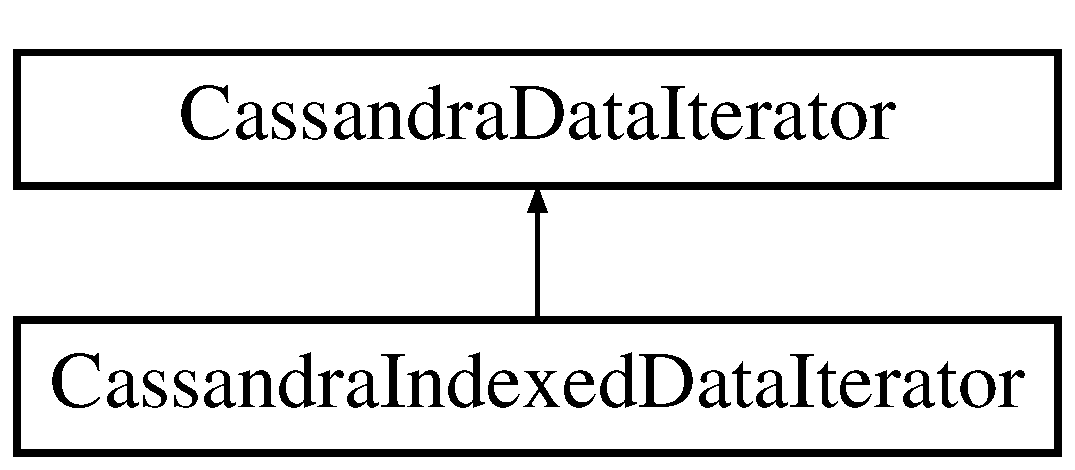
\includegraphics[height=2.000000cm]{classCassandraIndexedDataIterator}
\end{center}
\end{figure}
\subsection*{Public Member Functions}
\begin{DoxyCompactItemize}
\item 
\hyperlink{classCassandraIndexedDataIterator_a489fdf163525dd1bd4cf99b4e81708f3}{\_\-\_\-construct} (\hyperlink{classCassandraColumnFamily}{CassandraColumnFamily} \$columnFamily, cassandra\_\-ColumnParent \$columnParent, cassandra\_\-IndexClause \$indexClause, cassandra\_\-SlicePredicate \$slicePredicate, \$consistency, \$rowCountLimit, \$bufferSize)
\end{DoxyCompactItemize}
\subsection*{Protected Member Functions}
\begin{DoxyCompactItemize}
\item 
\hyperlink{classCassandraIndexedDataIterator_a1d38641286c86458941bca203d6fea65}{updateBuffer} ()
\end{DoxyCompactItemize}
\subsection*{Protected Attributes}
\begin{DoxyCompactItemize}
\item 
\hypertarget{classCassandraIndexedDataIterator_a21fda6e85a7d5d7dda9da9edf26be514}{
{\bfseries \$indexClause}}
\label{classCassandraIndexedDataIterator_a21fda6e85a7d5d7dda9da9edf26be514}

\end{DoxyCompactItemize}


\subsection{Detailed Description}
Indexed data iterator, used when performing where-\/queries. 

Definition at line 3455 of file Cassandra.php.



\subsection{Constructor \& Destructor Documentation}
\hypertarget{classCassandraIndexedDataIterator_a489fdf163525dd1bd4cf99b4e81708f3}{
\index{CassandraIndexedDataIterator@{CassandraIndexedDataIterator}!\_\-\_\-construct@{\_\-\_\-construct}}
\index{\_\-\_\-construct@{\_\-\_\-construct}!CassandraIndexedDataIterator@{CassandraIndexedDataIterator}}
\subsubsection[{\_\-\_\-construct}]{\setlength{\rightskip}{0pt plus 5cm}CassandraIndexedDataIterator::\_\-\_\-construct (
\begin{DoxyParamCaption}
\item[{{\bf CassandraColumnFamily} \$}]{columnFamily, }
\item[{cassandra\_\-ColumnParent \$}]{columnParent, }
\item[{cassandra\_\-IndexClause \$}]{indexClause, }
\item[{cassandra\_\-SlicePredicate \$}]{slicePredicate, }
\item[{\$}]{consistency, }
\item[{\$}]{rowCountLimit, }
\item[{\$}]{bufferSize}
\end{DoxyParamCaption}
)}}
\label{classCassandraIndexedDataIterator_a489fdf163525dd1bd4cf99b4e81708f3}
Sets the information needed to iterate the data in batches.


\begin{DoxyParams}[1]{Parameters}
\hyperlink{classCassandraColumnFamily}{CassandraColumnFamily} & {\em \$columnFamily} & Column family \\
\hline
cassandra\_\-ColumnParent & {\em \$columnParent} & Parent column \\
\hline
cassandra\_\-IndexClause & {\em \$indexClause} & The index clause to use \\
\hline
cassandra\_\-SlicePredicate & {\em \$slicePredicate} & Slice predicate \\
\hline
type & {\em \$startKey} & Key to start fetching data from \\
\hline
type & {\em \$consistency} & Consistency to use \\
\hline
type & {\em \$rowCountLimit} & Maximum number or rows to fetch \\
\hline
type & {\em \$bufferSize} & How many rows to fetch in a single request \\
\hline
\end{DoxyParams}


Definition at line 3476 of file Cassandra.php.


\begin{DoxyCode}
      {
        parent::__construct(
            $columnFamily,
            $columnParent,
            $slicePredicate,
            $indexClause->start_key,
            $consistency,
            $rowCountLimit, 
            $bufferSize
        );
        
        $this->indexClause = $indexClause;
    }
\end{DoxyCode}


\subsection{Member Function Documentation}
\hypertarget{classCassandraIndexedDataIterator_a1d38641286c86458941bca203d6fea65}{
\index{CassandraIndexedDataIterator@{CassandraIndexedDataIterator}!updateBuffer@{updateBuffer}}
\index{updateBuffer@{updateBuffer}!CassandraIndexedDataIterator@{CassandraIndexedDataIterator}}
\subsubsection[{updateBuffer}]{\setlength{\rightskip}{0pt plus 5cm}CassandraIndexedDataIterator::updateBuffer (
\begin{DoxyParamCaption}
{}
\end{DoxyParamCaption}
)\hspace{0.3cm}{\ttfamily  \mbox{[}protected\mbox{]}}}}
\label{classCassandraIndexedDataIterator_a1d38641286c86458941bca203d6fea65}
Updates the internal buffer, fetching new indexed data.

\begin{DoxyReturn}{Returns}
void 
\end{DoxyReturn}


Reimplemented from \hyperlink{classCassandraDataIterator_a20435cd4a3a06df86d62f9975933c808}{CassandraDataIterator}.



Definition at line 3503 of file Cassandra.php.


\begin{DoxyCode}
                                      {
        if ($this->rowCountLimit !== null) {
            $this->indexClause->count = min(
                $this->rowCountLimit - $this->rowsSeen + 1,
                $this->bufferSize
            );
        } else {
            $this->indexClause->count = $this->bufferSize;
        }
        
        $this->expectedPageSize = $this->indexClause->count;
        $this->indexClause->start_key = $this->nextStartKey;
        
        $result = $this->columnFamily->getCassandra()->call(
            'get_indexed_slices',
            $this->columnParent,
            $this->indexClause,
            $this->slicePredicate,
            $this->consistency
        );
        
        if (count($result) == 0) {
            $this->buffer = array();
        } else {
            $this->buffer = $this->columnFamily->parseSlicesResponse($result);
        }
        
        $this->currentPageSize = count($this->buffer);
    }
\end{DoxyCode}


The documentation for this class was generated from the following file:\begin{DoxyCompactItemize}
\item 
Cassandra.php\end{DoxyCompactItemize}

\hypertarget{classCassandraInvalidPatternException}{
\section{CassandraInvalidPatternException Class Reference}
\label{classCassandraInvalidPatternException}\index{CassandraInvalidPatternException@{CassandraInvalidPatternException}}
}


\subsection{Detailed Description}
Thrown if the \{\begin{DoxySeeAlso}{See also}
\hyperlink{classCassandra_ad2f8866d598ac0f696cb0c87258133fb}{Cassandra::get()}\} request pattern is invalid. 
\end{DoxySeeAlso}


Definition at line 3658 of file Cassandra.php.



The documentation for this class was generated from the following file:\begin{DoxyCompactItemize}
\item 
Cassandra.php\end{DoxyCompactItemize}

\hypertarget{classCassandraInvalidRequestException}{
\section{CassandraInvalidRequestException Class Reference}
\label{classCassandraInvalidRequestException}\index{CassandraInvalidRequestException@{CassandraInvalidRequestException}}
}


\subsection{Detailed Description}
Thrown if any kind of invalid parameters are provided. 

Definition at line 3653 of file Cassandra.php.



The documentation for this class was generated from the following file:\begin{DoxyCompactItemize}
\item 
Cassandra.php\end{DoxyCompactItemize}

\hypertarget{classCassandraMaxRetriesException}{
\section{CassandraMaxRetriesException Class Reference}
\label{classCassandraMaxRetriesException}\index{CassandraMaxRetriesException@{CassandraMaxRetriesException}}
}


\subsection{Detailed Description}
Thrown if maximum number of call retries is exceeded. 

Definition at line 3627 of file Cassandra.php.



The documentation for this class was generated from the following file:\begin{DoxyCompactItemize}
\item 
Cassandra.php\end{DoxyCompactItemize}

\hypertarget{classCassandraRangeDataIterator}{
\section{CassandraRangeDataIterator Class Reference}
\label{classCassandraRangeDataIterator}\index{CassandraRangeDataIterator@{CassandraRangeDataIterator}}
}
Inheritance diagram for CassandraRangeDataIterator:\begin{figure}[H]
\begin{center}
\leavevmode
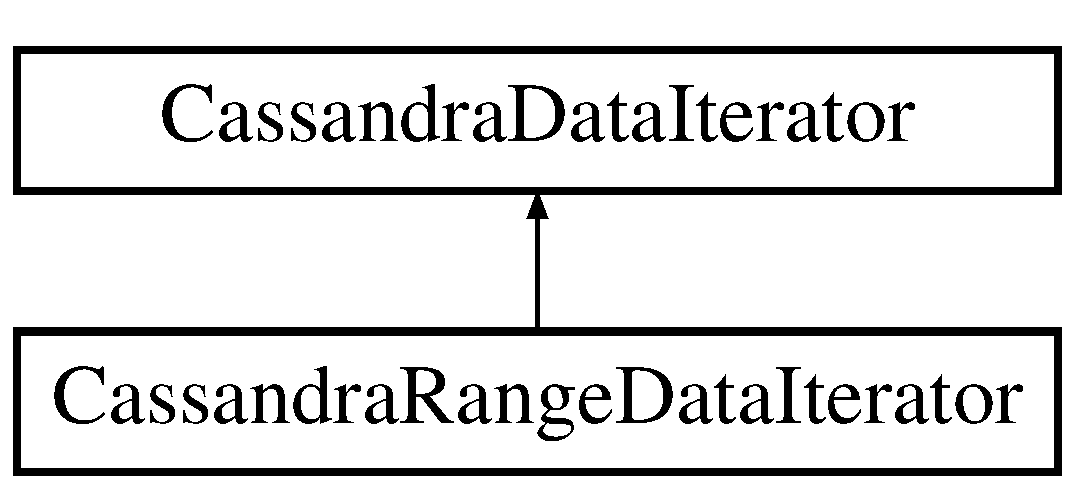
\includegraphics[height=2.000000cm]{classCassandraRangeDataIterator}
\end{center}
\end{figure}
\subsection*{Public Member Functions}
\begin{DoxyCompactItemize}
\item 
\hyperlink{classCassandraRangeDataIterator_a89ad9afec67135eed73321396c6581b1}{\_\-\_\-construct} (\hyperlink{classCassandraColumnFamily}{CassandraColumnFamily} \$columnFamily, cassandra\_\-ColumnParent \$columnParent, cassandra\_\-SlicePredicate \$slicePredicate, \$startKey, \$endKey, \$consistency, \$rowCountLimit, \$bufferSize)
\end{DoxyCompactItemize}
\subsection*{Protected Member Functions}
\begin{DoxyCompactItemize}
\item 
\hyperlink{classCassandraRangeDataIterator_a743234ebb424200a5c3d7473ce95dbba}{updateBuffer} ()
\end{DoxyCompactItemize}
\subsection*{Protected Attributes}
\begin{DoxyCompactItemize}
\item 
\hypertarget{classCassandraRangeDataIterator_ac977d1d6c76e705920dc8394a00009c5}{
{\bfseries \$startKey}}
\label{classCassandraRangeDataIterator_ac977d1d6c76e705920dc8394a00009c5}

\item 
\hypertarget{classCassandraRangeDataIterator_acd5cccd82a215f9a2becd2cf4f635a50}{
{\bfseries \$endKey}}
\label{classCassandraRangeDataIterator_acd5cccd82a215f9a2becd2cf4f635a50}

\end{DoxyCompactItemize}


\subsection{Detailed Description}
Key range data iterator. 

Definition at line 3537 of file Cassandra.php.



\subsection{Constructor \& Destructor Documentation}
\hypertarget{classCassandraRangeDataIterator_a89ad9afec67135eed73321396c6581b1}{
\index{CassandraRangeDataIterator@{CassandraRangeDataIterator}!\_\-\_\-construct@{\_\-\_\-construct}}
\index{\_\-\_\-construct@{\_\-\_\-construct}!CassandraRangeDataIterator@{CassandraRangeDataIterator}}
\subsubsection[{\_\-\_\-construct}]{\setlength{\rightskip}{0pt plus 5cm}CassandraRangeDataIterator::\_\-\_\-construct (
\begin{DoxyParamCaption}
\item[{{\bf CassandraColumnFamily} \$}]{columnFamily, }
\item[{cassandra\_\-ColumnParent \$}]{columnParent, }
\item[{cassandra\_\-SlicePredicate \$}]{slicePredicate, }
\item[{\$}]{startKey, }
\item[{\$}]{endKey, }
\item[{\$}]{consistency, }
\item[{\$}]{rowCountLimit, }
\item[{\$}]{bufferSize}
\end{DoxyParamCaption}
)}}
\label{classCassandraRangeDataIterator_a89ad9afec67135eed73321396c6581b1}
Sets the information needed to iterate the data in batches.


\begin{DoxyParams}[1]{Parameters}
\hyperlink{classCassandraColumnFamily}{CassandraColumnFamily} & {\em \$columnFamily} & Column family \\
\hline
cassandra\_\-ColumnParent & {\em \$columnParent} & Parent column \\
\hline
cassandra\_\-SlicePredicate & {\em \$slicePredicate} & Slice predicate \\
\hline
type & {\em \$startKey} & Key to start fetching data from \\
\hline
type & {\em \$emdKey} & Last key to fetch in a range \\
\hline
type & {\em \$consistency} & Consistency to use \\
\hline
type & {\em \$rowCountLimit} & Maximum number or rows to fetch \\
\hline
type & {\em \$bufferSize} & How many rows to fetch in a single request \\
\hline
\end{DoxyParams}


Definition at line 3565 of file Cassandra.php.


\begin{DoxyCode}
      {
        parent::__construct(
            $columnFamily,
            $columnParent,
            $slicePredicate,
            $startKey,
            $consistency,
            $rowCountLimit, 
            $bufferSize
        );
        
        $this->startKey = $startKey;
        $this->endKey = $endKey;
    }
\end{DoxyCode}


\subsection{Member Function Documentation}
\hypertarget{classCassandraRangeDataIterator_a743234ebb424200a5c3d7473ce95dbba}{
\index{CassandraRangeDataIterator@{CassandraRangeDataIterator}!updateBuffer@{updateBuffer}}
\index{updateBuffer@{updateBuffer}!CassandraRangeDataIterator@{CassandraRangeDataIterator}}
\subsubsection[{updateBuffer}]{\setlength{\rightskip}{0pt plus 5cm}CassandraRangeDataIterator::updateBuffer (
\begin{DoxyParamCaption}
{}
\end{DoxyParamCaption}
)\hspace{0.3cm}{\ttfamily  \mbox{[}protected\mbox{]}}}}
\label{classCassandraRangeDataIterator_a743234ebb424200a5c3d7473ce95dbba}
Updates the internal buffer, fetching new ranged data.

\begin{DoxyReturn}{Returns}
void 
\end{DoxyReturn}


Reimplemented from \hyperlink{classCassandraDataIterator_a20435cd4a3a06df86d62f9975933c808}{CassandraDataIterator}.



Definition at line 3594 of file Cassandra.php.


\begin{DoxyCode}
                                      {
        $bufferSize = $this->bufferSize;
        
        if ($this->rowCountLimit !== null) {
            $bufferSize = min(
                $this->rowCountLimit - $this->rowsSeen + 1,
                $this->bufferSize
            );
        }
        
        $this->expectedPageSize = $bufferSize;
        
        $keyRange = new cassandra_KeyRange();
        $keyRange->start_key = $this->nextStartKey;
        $keyRange->end_key = $this->endKey;
        $keyRange->count = $bufferSize;
        
        $result = $this->columnFamily->getCassandra()->call(
            'get_range_slices',
            $this->columnParent,
            $this->slicePredicate,
            $keyRange,
            $this->consistency
        );
        
        $this->buffer = $this->columnFamily->parseSlicesResponse($result);
        $this->currentPageSize = count($this->buffer);
    }
\end{DoxyCode}


The documentation for this class was generated from the following file:\begin{DoxyCompactItemize}
\item 
Cassandra.php\end{DoxyCompactItemize}

\hypertarget{classCassandraSettingKeyspaceFailedException}{
\section{CassandraSettingKeyspaceFailedException Class Reference}
\label{classCassandraSettingKeyspaceFailedException}\index{CassandraSettingKeyspaceFailedException@{CassandraSettingKeyspaceFailedException}}
}


\subsection{Detailed Description}
Thrown if using the requested keyspace failed. 

Definition at line 3643 of file Cassandra.php.



The documentation for this class was generated from the following file:\begin{DoxyCompactItemize}
\item 
Cassandra.php\end{DoxyCompactItemize}

\hypertarget{classCassandraUnsupportedException}{
\section{CassandraUnsupportedException Class Reference}
\label{classCassandraUnsupportedException}\index{CassandraUnsupportedException@{CassandraUnsupportedException}}
}


\subsection{Detailed Description}
Thrown if requested method is not supported by \hyperlink{classCassandra}{Cassandra} or this library 

Definition at line 3663 of file Cassandra.php.



The documentation for this class was generated from the following file:\begin{DoxyCompactItemize}
\item 
Cassandra.php\end{DoxyCompactItemize}

\hypertarget{classCassandraUtil}{
\section{CassandraUtil Class Reference}
\label{classCassandraUtil}\index{CassandraUtil@{CassandraUtil}}
}
\subsection*{Public Member Functions}
\begin{DoxyCompactItemize}
\item 
\hyperlink{classCassandraUtil_ad5c94f8a7e99e7240385cf471c2b4ae8}{getTimestamp} ()
\end{DoxyCompactItemize}
\subsection*{Static Public Member Functions}
\begin{DoxyCompactItemize}
\item 
static \hyperlink{classCassandraUtil_a0c6545c1306d917051a53598a0f23ee6}{extractType} (\$definition)
\item 
static \hyperlink{classCassandraUtil_aa70ff00c6c785127c87a46c966999e66}{pack} (\$value, \$type)
\item 
static \hyperlink{classCassandraUtil_a92f49d16f99991a04a3f798ee91f7d0b}{packLong} (\$value)
\item 
static \hyperlink{classCassandraUtil_aa5b20568dcda475aba51dc1ac6bdfcb1}{packInteger} (\$value)
\item 
static \hyperlink{classCassandraUtil_a5e6486c8b5438bf565f13789f0403053}{packString} (\$string, \$length)
\item 
static \hyperlink{classCassandraUtil_a0e4efa10d6999de6fbbc2efa3f24a089}{unpack} (\$value, \$type)
\item 
static \hyperlink{classCassandraUtil_a8753dea96e94a3c84d8e5aada1418dbb}{unpackLong} (\$data)
\item 
static \hyperlink{classCassandraUtil_ab0dcf37a5de9d22e665ca291a3afd4a2}{unpackInteger} (\$value)
\item 
static \hyperlink{classCassandraUtil_ab49d399bb60d2e0094de49b77cd00dbe}{unpackString} (\$value, \$length)
\end{DoxyCompactItemize}


\subsection{Detailed Description}
Utility class for the \hyperlink{classCassandra}{Cassandra} library, providing some common operations like packing data to correct type.

Includes quite a lot of code from PHPCassa project. 

Definition at line 2888 of file Cassandra.php.



\subsection{Member Function Documentation}
\hypertarget{classCassandraUtil_a0c6545c1306d917051a53598a0f23ee6}{
\index{CassandraUtil@{CassandraUtil}!extractType@{extractType}}
\index{extractType@{extractType}!CassandraUtil@{CassandraUtil}}
\subsubsection[{extractType}]{\setlength{\rightskip}{0pt plus 5cm}static CassandraUtil::extractType (
\begin{DoxyParamCaption}
\item[{\$}]{definition}
\end{DoxyParamCaption}
)\hspace{0.3cm}{\ttfamily  \mbox{[}static\mbox{]}}}}
\label{classCassandraUtil_a0c6545c1306d917051a53598a0f23ee6}
Extracts the data type name from given definition.

The parsed names match the constancts Cassandra::TYPE\_\-...


\begin{DoxyParams}[1]{Parameters}
string & {\em \$definition} & Definition to parse \\
\hline
\end{DoxyParams}
\begin{DoxyReturn}{Returns}
string Valid data type name 
\end{DoxyReturn}


Definition at line 2898 of file Cassandra.php.


\begin{DoxyCode}
                                                    {
        if ($definition === null or $definition == '') {
            return Cassandra::TYPE_BYTES;
        }

        $index = strrpos($definition, '.');

        if ($index === false) {
            return Cassandra::TYPE_BYTES;
        }

        return substr($definition, $index + 1);
    }
\end{DoxyCode}
\hypertarget{classCassandraUtil_ad5c94f8a7e99e7240385cf471c2b4ae8}{
\index{CassandraUtil@{CassandraUtil}!getTimestamp@{getTimestamp}}
\index{getTimestamp@{getTimestamp}!CassandraUtil@{CassandraUtil}}
\subsubsection[{getTimestamp}]{\setlength{\rightskip}{0pt plus 5cm}CassandraUtil::getTimestamp (
\begin{DoxyParamCaption}
{}
\end{DoxyParamCaption}
)}}
\label{classCassandraUtil_ad5c94f8a7e99e7240385cf471c2b4ae8}
Returns current timestamp that can be used in insert/update opearations.

By Zach Buller (\href{mailto:zachbuller@gmail.com}{\tt zachbuller@gmail.com})

\begin{DoxyReturn}{Returns}
integer Unpacked data 
\end{DoxyReturn}


Definition at line 3156 of file Cassandra.php.


\begin{DoxyCode}
                                   {
        $microtime = microtime();
        
        settype($microtime, 'string');
        
        $timeTokens = explode(" ", $microtime);
        $subSeconds = preg_replace('/0./', '', $timeTokens[0], 1);
        
        return ($timeTokens[1].$subSeconds) / 100;
    }
\end{DoxyCode}
\hypertarget{classCassandraUtil_aa70ff00c6c785127c87a46c966999e66}{
\index{CassandraUtil@{CassandraUtil}!pack@{pack}}
\index{pack@{pack}!CassandraUtil@{CassandraUtil}}
\subsubsection[{pack}]{\setlength{\rightskip}{0pt plus 5cm}static CassandraUtil::pack (
\begin{DoxyParamCaption}
\item[{\$}]{value, }
\item[{\$}]{type}
\end{DoxyParamCaption}
)\hspace{0.3cm}{\ttfamily  \mbox{[}static\mbox{]}}}}
\label{classCassandraUtil_aa70ff00c6c785127c87a46c966999e66}
Packs given value to given type.


\begin{DoxyParams}[1]{Parameters}
mixed & {\em \$value} & Value to pack \\
\hline
string & {\em \$type} & Type name to pack to \\
\hline
\end{DoxyParams}
\begin{DoxyReturn}{Returns}
mixed Data packed to requested type 
\end{DoxyReturn}


Definition at line 2919 of file Cassandra.php.


\begin{DoxyCode}
                                               {
        switch ($type) {
            case Cassandra::TYPE_LONG:
                return self::packLong($value);
            
            case Cassandra::TYPE_INTEGER:
                return self::packInteger($value);
            
            case Cassandra::TYPE_ASCII:
                return self::packString($value, strlen($value));
            
            case Cassandra::TYPE_UTF8:
                if (mb_detect_encoding($value, 'UTF-8') != 'UTF-8') {
                    $value = utf8_encode($value);
                }
                
                return self::packString($value, strlen($value));
                
            case Cassandra::TYPE_TIME_UUID:
                return self::packString($value, 16);
            
            case Cassandra::TYPE_LEXICAL_UUID:
                return self::packString($value, 16);
                
            default:
                return $value;
        }
    }
\end{DoxyCode}
\hypertarget{classCassandraUtil_aa5b20568dcda475aba51dc1ac6bdfcb1}{
\index{CassandraUtil@{CassandraUtil}!packInteger@{packInteger}}
\index{packInteger@{packInteger}!CassandraUtil@{CassandraUtil}}
\subsubsection[{packInteger}]{\setlength{\rightskip}{0pt plus 5cm}static CassandraUtil::packInteger (
\begin{DoxyParamCaption}
\item[{\$}]{value}
\end{DoxyParamCaption}
)\hspace{0.3cm}{\ttfamily  \mbox{[}static\mbox{]}}}}
\label{classCassandraUtil_aa5b20568dcda475aba51dc1ac6bdfcb1}
Packs data to integer type.


\begin{DoxyParams}[1]{Parameters}
mixed & {\em \$value} & Value to pack \\
\hline
\end{DoxyParams}
\begin{DoxyReturn}{Returns}
integer Packed data 
\end{DoxyReturn}


Definition at line 2997 of file Cassandra.php.


\begin{DoxyCode}
                                               {
        return pack('N', $value);
    }
\end{DoxyCode}
\hypertarget{classCassandraUtil_a92f49d16f99991a04a3f798ee91f7d0b}{
\index{CassandraUtil@{CassandraUtil}!packLong@{packLong}}
\index{packLong@{packLong}!CassandraUtil@{CassandraUtil}}
\subsubsection[{packLong}]{\setlength{\rightskip}{0pt plus 5cm}static CassandraUtil::packLong (
\begin{DoxyParamCaption}
\item[{\$}]{value}
\end{DoxyParamCaption}
)\hspace{0.3cm}{\ttfamily  \mbox{[}static\mbox{]}}}}
\label{classCassandraUtil_a92f49d16f99991a04a3f798ee91f7d0b}
Packs data to long type.


\begin{DoxyParams}[1]{Parameters}
mixed & {\em \$value} & Value to pack \\
\hline
\end{DoxyParams}
\begin{DoxyReturn}{Returns}
integer Packed data 
\end{DoxyReturn}


Definition at line 2954 of file Cassandra.php.


\begin{DoxyCode}
                                            {
        // If we are on a 32bit architecture we have to explicitly deal with
        // 64-bit twos-complement arithmetic since PHP wants to treat all ints
        // as signed and any int over 2^31 - 1 as a float
        if (PHP_INT_SIZE == 4) {
            $neg = $value < 0;

            if ($neg) {
                $value *= - 1;
            }

            $hi = (int) ($value / 4294967296);
            $lo = (int) $value;

            if ($neg) {
                $hi = ~$hi;
                $lo = ~$lo;
                
                if (($lo & (int)0xffffffff) == (int)0xffffffff) {
                    $lo = 0;
                    $hi++;
                } else {
                    $lo++;
                }
            }
            
            $data = pack('N2', $hi, $lo);
        } else {
            $hi = $value >> 32;
            $lo = $value & 0xFFFFFFFF;
            
            $data = pack('N2', $hi, $lo);
        }
        
        return $data;
    }
\end{DoxyCode}
\hypertarget{classCassandraUtil_a5e6486c8b5438bf565f13789f0403053}{
\index{CassandraUtil@{CassandraUtil}!packString@{packString}}
\index{packString@{packString}!CassandraUtil@{CassandraUtil}}
\subsubsection[{packString}]{\setlength{\rightskip}{0pt plus 5cm}static CassandraUtil::packString (
\begin{DoxyParamCaption}
\item[{\$}]{string, }
\item[{\$}]{length}
\end{DoxyParamCaption}
)\hspace{0.3cm}{\ttfamily  \mbox{[}static\mbox{]}}}}
\label{classCassandraUtil_a5e6486c8b5438bf565f13789f0403053}
Packs data to string type.


\begin{DoxyParams}[1]{Parameters}
mixed & {\em \$value} & Value to pack \\
\hline
\end{DoxyParams}
\begin{DoxyReturn}{Returns}
string Packed data 
\end{DoxyReturn}


Definition at line 3007 of file Cassandra.php.


\begin{DoxyCode}
                                                        {       
        $result = '';
        
        for($i = 0; $i < $length; $i++) {
            $result .= pack('c', ord(substr($string, $i, 1)));
        }
        
        return $result;
    }
\end{DoxyCode}
\hypertarget{classCassandraUtil_a0e4efa10d6999de6fbbc2efa3f24a089}{
\index{CassandraUtil@{CassandraUtil}!unpack@{unpack}}
\index{unpack@{unpack}!CassandraUtil@{CassandraUtil}}
\subsubsection[{unpack}]{\setlength{\rightskip}{0pt plus 5cm}static CassandraUtil::unpack (
\begin{DoxyParamCaption}
\item[{\$}]{value, }
\item[{\$}]{type}
\end{DoxyParamCaption}
)\hspace{0.3cm}{\ttfamily  \mbox{[}static\mbox{]}}}}
\label{classCassandraUtil_a0e4efa10d6999de6fbbc2efa3f24a089}
Unpacks packed data from given type to something PHP understands.


\begin{DoxyParams}[1]{Parameters}
string & {\em \$value} & Value to unpack \\
\hline
string & {\em \$type} & Current type of the data \\
\hline
\end{DoxyParams}
\begin{DoxyReturn}{Returns}
mixed Unpacked data 
\end{DoxyReturn}


Definition at line 3024 of file Cassandra.php.


\begin{DoxyCode}
                                                 {
        switch ($type) {
            case Cassandra::TYPE_LONG:
                return self::unpackLong($value);
            
            case Cassandra::TYPE_INTEGER:
                return self::unpackInteger($value);
            
            case Cassandra::TYPE_ASCII:
                return self::unpackString($value, strlen($value));
            
            case Cassandra::TYPE_UTF8:
                return self::unpackString($value, strlen($value));
                
            case Cassandra::TYPE_TIME_UUID:
                return $value;
            
            case Cassandra::TYPE_LEXICAL_UUID:
                return $value;
                
            default:
                return $value;
        }
    }
\end{DoxyCode}
\hypertarget{classCassandraUtil_ab0dcf37a5de9d22e665ca291a3afd4a2}{
\index{CassandraUtil@{CassandraUtil}!unpackInteger@{unpackInteger}}
\index{unpackInteger@{unpackInteger}!CassandraUtil@{CassandraUtil}}
\subsubsection[{unpackInteger}]{\setlength{\rightskip}{0pt plus 5cm}static CassandraUtil::unpackInteger (
\begin{DoxyParamCaption}
\item[{\$}]{value}
\end{DoxyParamCaption}
)\hspace{0.3cm}{\ttfamily  \mbox{[}static\mbox{]}}}}
\label{classCassandraUtil_ab0dcf37a5de9d22e665ca291a3afd4a2}
Unpacks integer data type.


\begin{DoxyParams}[1]{Parameters}
mixed & {\em \$data} & Data to unpack \\
\hline
\end{DoxyParams}
\begin{DoxyReturn}{Returns}
integer Unpacked data 
\end{DoxyReturn}


Definition at line 3124 of file Cassandra.php.


\begin{DoxyCode}
                                                 {
        $unpacked = unpack('N', $value);
        
        return array_pop($unpacked);
    }
\end{DoxyCode}
\hypertarget{classCassandraUtil_a8753dea96e94a3c84d8e5aada1418dbb}{
\index{CassandraUtil@{CassandraUtil}!unpackLong@{unpackLong}}
\index{unpackLong@{unpackLong}!CassandraUtil@{CassandraUtil}}
\subsubsection[{unpackLong}]{\setlength{\rightskip}{0pt plus 5cm}static CassandraUtil::unpackLong (
\begin{DoxyParamCaption}
\item[{\$}]{data}
\end{DoxyParamCaption}
)\hspace{0.3cm}{\ttfamily  \mbox{[}static\mbox{]}}}}
\label{classCassandraUtil_a8753dea96e94a3c84d8e5aada1418dbb}
Unpacks long data type.


\begin{DoxyParams}[1]{Parameters}
mixed & {\em \$data} & Data to unpack \\
\hline
\end{DoxyParams}
\begin{DoxyReturn}{Returns}
integer Unpacked data 
\end{DoxyReturn}


Definition at line 3055 of file Cassandra.php.


\begin{DoxyCode}
                                             {
        $arr = unpack('N2', $data);

        // If we are on a 32bit architecture we have to explicitly deal with
        // 64-bit twos-complement arithmetic since PHP wants to treat all ints
        // as signed and any int over 2^31 - 1 as a float
        if (PHP_INT_SIZE == 4) {

            $hi = $arr[1];
            $lo = $arr[2];
            $isNeg = $hi < 0;

            // Check for a negative
            if ($isNeg) {
                $hi = ~$hi & (int)0xffffffff;
                $lo = ~$lo & (int)0xffffffff;

                if ($lo == (int)0xffffffff) {
                    $hi++;
                    $lo = 0;
                } else {
                    $lo++;
                }
            }

            // Force 32bit words in excess of 2G to pe positive - we deal wigh
            // sign explicitly below

            if ($hi & (int)0x80000000) {
                $hi &= (int)0x7fffffff;
                $hi += 0x80000000;
            }

            if ($lo & (int)0x80000000) {
                $lo &= (int)0x7fffffff;
                $lo += 0x80000000;
            }

            $value = $hi * 4294967296 + $lo;

            if ($isNeg) {
                $value = 0 - $value;
            }
        } else {
            // Upcast negatives in LSB bit
            if ($arr[2] & 0x80000000)
                $arr[2] = $arr[2] & 0xffffffff;

            // Check for a negative
            if ($arr[1] & 0x80000000) {
                $arr[1] = $arr[1] & 0xffffffff;
                $arr[1] = $arr[1] ^ 0xffffffff;
                $arr[2] = $arr[2] ^ 0xffffffff;
                
                $value = 0 - $arr[1] * 4294967296 - $arr[2] - 1;
            } else {
                $value = $arr[1] * 4294967296 + $arr[2];
            }
        }
        
        return $value;
    }
\end{DoxyCode}
\hypertarget{classCassandraUtil_ab49d399bb60d2e0094de49b77cd00dbe}{
\index{CassandraUtil@{CassandraUtil}!unpackString@{unpackString}}
\index{unpackString@{unpackString}!CassandraUtil@{CassandraUtil}}
\subsubsection[{unpackString}]{\setlength{\rightskip}{0pt plus 5cm}static CassandraUtil::unpackString (
\begin{DoxyParamCaption}
\item[{\$}]{value, }
\item[{\$}]{length}
\end{DoxyParamCaption}
)\hspace{0.3cm}{\ttfamily  \mbox{[}static\mbox{]}}}}
\label{classCassandraUtil_ab49d399bb60d2e0094de49b77cd00dbe}
Unpacks string data type.


\begin{DoxyParams}[1]{Parameters}
mixed & {\em \$data} & Data to unpack \\
\hline
\end{DoxyParams}
\begin{DoxyReturn}{Returns}
string Unpacked data 
\end{DoxyReturn}


Definition at line 3136 of file Cassandra.php.


\begin{DoxyCode}
                                                         {
        $unpacked = unpack('c'.$length.'chars', $value);
        $out = '';
        
        foreach($unpacked as $element) {
            if($element > 0) {
                $out .= chr($element);
            }
        }
        
        return $out;
    }
\end{DoxyCode}


The documentation for this class was generated from the following file:\begin{DoxyCompactItemize}
\item 
Cassandra.php\end{DoxyCompactItemize}

\printindex
\end{document}
